% Options for packages loaded elsewhere
% Options for packages loaded elsewhere
\PassOptionsToPackage{unicode}{hyperref}
\PassOptionsToPackage{hyphens}{url}
\PassOptionsToPackage{dvipsnames,svgnames,x11names}{xcolor}
%
\documentclass[
  russian,
  12pt,
  a4paper,
  a4paper,
  openany]{scrbook}
\usepackage{xcolor}
\usepackage[inner=25mm,outer=25mm,top=22mm,bottom=24mm,headheight=13pt,headsep=8mm]{geometry}
\usepackage{amsmath,amssymb}
\setcounter{secnumdepth}{-\maxdimen} % remove section numbering
\usepackage{iftex}
\ifPDFTeX
  \usepackage[T1]{fontenc}
  \usepackage[utf8]{inputenc}
  \usepackage{textcomp} % provide euro and other symbols
\else % if luatex or xetex
  \usepackage{unicode-math} % this also loads fontspec
  \defaultfontfeatures{Scale=MatchLowercase}
  \defaultfontfeatures[\rmfamily]{Ligatures=TeX,Scale=1}
\fi
\usepackage{lmodern}
\ifPDFTeX\else
  % xetex/luatex font selection
\fi
% Use upquote if available, for straight quotes in verbatim environments
\IfFileExists{upquote.sty}{\usepackage{upquote}}{}
\IfFileExists{microtype.sty}{% use microtype if available
  \usepackage[]{microtype}
  \UseMicrotypeSet[protrusion]{basicmath} % disable protrusion for tt fonts
}{}
\makeatletter
\@ifundefined{KOMAClassName}{% if non-KOMA class
  \IfFileExists{parskip.sty}{%
    \usepackage{parskip}
  }{% else
    \setlength{\parindent}{0pt}
    \setlength{\parskip}{6pt plus 2pt minus 1pt}}
}{% if KOMA class
  \KOMAoptions{parskip=half}}
\makeatother
% Make \paragraph and \subparagraph free-standing
\makeatletter
\ifx\paragraph\undefined\else
  \let\oldparagraph\paragraph
  \renewcommand{\paragraph}{
    \@ifstar
      \xxxParagraphStar
      \xxxParagraphNoStar
  }
  \newcommand{\xxxParagraphStar}[1]{\oldparagraph*{#1}\mbox{}}
  \newcommand{\xxxParagraphNoStar}[1]{\oldparagraph{#1}\mbox{}}
\fi
\ifx\subparagraph\undefined\else
  \let\oldsubparagraph\subparagraph
  \renewcommand{\subparagraph}{
    \@ifstar
      \xxxSubParagraphStar
      \xxxSubParagraphNoStar
  }
  \newcommand{\xxxSubParagraphStar}[1]{\oldsubparagraph*{#1}\mbox{}}
  \newcommand{\xxxSubParagraphNoStar}[1]{\oldsubparagraph{#1}\mbox{}}
\fi
\makeatother

\usepackage{color}
\usepackage{fancyvrb}
\newcommand{\VerbBar}{|}
\newcommand{\VERB}{\Verb[commandchars=\\\{\}]}
\DefineVerbatimEnvironment{Highlighting}{Verbatim}{commandchars=\\\{\}}
% Add ',fontsize=\small' for more characters per line
\usepackage{framed}
\definecolor{shadecolor}{RGB}{241,243,245}
\newenvironment{Shaded}{\begin{snugshade}}{\end{snugshade}}
\newcommand{\AlertTok}[1]{\textcolor[rgb]{0.68,0.00,0.00}{#1}}
\newcommand{\AnnotationTok}[1]{\textcolor[rgb]{0.37,0.37,0.37}{#1}}
\newcommand{\AttributeTok}[1]{\textcolor[rgb]{0.40,0.45,0.13}{#1}}
\newcommand{\BaseNTok}[1]{\textcolor[rgb]{0.68,0.00,0.00}{#1}}
\newcommand{\BuiltInTok}[1]{\textcolor[rgb]{0.00,0.23,0.31}{#1}}
\newcommand{\CharTok}[1]{\textcolor[rgb]{0.13,0.47,0.30}{#1}}
\newcommand{\CommentTok}[1]{\textcolor[rgb]{0.37,0.37,0.37}{#1}}
\newcommand{\CommentVarTok}[1]{\textcolor[rgb]{0.37,0.37,0.37}{\textit{#1}}}
\newcommand{\ConstantTok}[1]{\textcolor[rgb]{0.56,0.35,0.01}{#1}}
\newcommand{\ControlFlowTok}[1]{\textcolor[rgb]{0.00,0.23,0.31}{\textbf{#1}}}
\newcommand{\DataTypeTok}[1]{\textcolor[rgb]{0.68,0.00,0.00}{#1}}
\newcommand{\DecValTok}[1]{\textcolor[rgb]{0.68,0.00,0.00}{#1}}
\newcommand{\DocumentationTok}[1]{\textcolor[rgb]{0.37,0.37,0.37}{\textit{#1}}}
\newcommand{\ErrorTok}[1]{\textcolor[rgb]{0.68,0.00,0.00}{#1}}
\newcommand{\ExtensionTok}[1]{\textcolor[rgb]{0.00,0.23,0.31}{#1}}
\newcommand{\FloatTok}[1]{\textcolor[rgb]{0.68,0.00,0.00}{#1}}
\newcommand{\FunctionTok}[1]{\textcolor[rgb]{0.28,0.35,0.67}{#1}}
\newcommand{\ImportTok}[1]{\textcolor[rgb]{0.00,0.46,0.62}{#1}}
\newcommand{\InformationTok}[1]{\textcolor[rgb]{0.37,0.37,0.37}{#1}}
\newcommand{\KeywordTok}[1]{\textcolor[rgb]{0.00,0.23,0.31}{\textbf{#1}}}
\newcommand{\NormalTok}[1]{\textcolor[rgb]{0.00,0.23,0.31}{#1}}
\newcommand{\OperatorTok}[1]{\textcolor[rgb]{0.37,0.37,0.37}{#1}}
\newcommand{\OtherTok}[1]{\textcolor[rgb]{0.00,0.23,0.31}{#1}}
\newcommand{\PreprocessorTok}[1]{\textcolor[rgb]{0.68,0.00,0.00}{#1}}
\newcommand{\RegionMarkerTok}[1]{\textcolor[rgb]{0.00,0.23,0.31}{#1}}
\newcommand{\SpecialCharTok}[1]{\textcolor[rgb]{0.37,0.37,0.37}{#1}}
\newcommand{\SpecialStringTok}[1]{\textcolor[rgb]{0.13,0.47,0.30}{#1}}
\newcommand{\StringTok}[1]{\textcolor[rgb]{0.13,0.47,0.30}{#1}}
\newcommand{\VariableTok}[1]{\textcolor[rgb]{0.07,0.07,0.07}{#1}}
\newcommand{\VerbatimStringTok}[1]{\textcolor[rgb]{0.13,0.47,0.30}{#1}}
\newcommand{\WarningTok}[1]{\textcolor[rgb]{0.37,0.37,0.37}{\textit{#1}}}

\usepackage{longtable,booktabs,array}
\newcounter{none} % for unnumbered tables
\usepackage{calc} % for calculating minipage widths
% Correct order of tables after \paragraph or \subparagraph
\usepackage{etoolbox}
\makeatletter
\patchcmd\longtable{\par}{\if@noskipsec\mbox{}\fi\par}{}{}
\makeatother
% Allow footnotes in longtable head/foot
\IfFileExists{footnotehyper.sty}{\usepackage{footnotehyper}}{\usepackage{footnote}}
\makesavenoteenv{longtable}
\usepackage{graphicx}
\makeatletter
\newsavebox\pandoc@box
\newcommand*\pandocbounded[1]{% scales image to fit in text height/width
  \sbox\pandoc@box{#1}%
  \Gscale@div\@tempa{\textheight}{\dimexpr\ht\pandoc@box+\dp\pandoc@box\relax}%
  \Gscale@div\@tempb{\linewidth}{\wd\pandoc@box}%
  \ifdim\@tempb\p@<\@tempa\p@\let\@tempa\@tempb\fi% select the smaller of both
  \ifdim\@tempa\p@<\p@\scalebox{\@tempa}{\usebox\pandoc@box}%
  \else\usebox{\pandoc@box}%
  \fi%
}
% Set default figure placement to htbp
\def\fps@figure{htbp}
\makeatother



\ifLuaTeX
\usepackage[bidi=basic,shorthands=off,provide=*]{babel}
\else
\usepackage[bidi=default,shorthands=off,provide=*]{babel}
\fi
\ifLuaTeX
  \usepackage{selnolig} % disable illegal ligatures
\fi


\setlength{\emergencystretch}{3em} % prevent overfull lines

\providecommand{\tightlist}{%
  \setlength{\itemsep}{0pt}\setlength{\parskip}{0pt}}



 


\usepackage{fontspec}
\usepackage{polyglossia}
\usepackage{unicode-math}
\usepackage{amsmath}
\usepackage{mathtools}
\usepackage{graphicx}
\usepackage{float}
\usepackage{booktabs}
\usepackage{longtable}
\usepackage{array}
\usepackage{microtype}
\usepackage{hyperref}

\defaultfontfeatures{Ligatures=TeX, Scale=MatchLowercase}
\setmainfont{Libertinus Serif}
\setsansfont{Libertinus Sans}
\setmonofont{Libertinus Mono}[Scale=0.9]
\setmathfont{Libertinus Math}

\setlength{\emergencystretch}{3em}

\hypersetup{
  pdfborder={0 0 0},
  colorlinks=true,
  linkcolor=black,
  citecolor=black,
  urlcolor=black
}

\newcommand{\E}{\mathbb{E}}
\newcommand{\Var}{\operatorname{Var}}
\newcommand{\cov}{\operatorname{cov}}
\newcommand{\dd}{\,\mathrm{d}}
\setmainlanguage{russian}
\setotherlanguage{english}
\PolyglossiaSetup{russian}{
  bcp47=ru,
  scripttag=cyrl,
  langtag=RUS,
  hyphennames={russian},
  hyphenmins={2,2},
  frenchspacing=true,
  indentfirst=true
}
% PDF visual theme for the statistical-analysis-course book.
% It mirrors the palette and visual language from assets/styles/book.css,
% while keeping the PDF close to the supplied reference edition.

\usepackage[most]{tcolorbox}
\usepackage{scrlayer-scrpage}
\usepackage{tikz}
\usepackage{caption}
\usepackage{colortbl}
\usepackage{array}
\usepackage{enumitem}
\usepackage{etoolbox}
\usepackage{ragged2e}

% -----------------------------------------------------------------------------
% Palette (same core colors as book.css)
% -----------------------------------------------------------------------------
\definecolor{BookInk}{HTML}{18262F}
\definecolor{BookInkSoft}{HTML}{42545F}
\definecolor{BookMuted}{HTML}{687984}
\definecolor{BookPaper}{HTML}{FFFFFF}
\definecolor{BookCanvas}{HTML}{F4F6F7}
\definecolor{BookLine}{HTML}{D9E0E3}
\definecolor{BookLineStrong}{HTML}{BCC9CE}
\definecolor{BookTeal}{HTML}{0F6972}
\definecolor{BookTealDark}{HTML}{094B52}
\definecolor{BookTealSoft}{HTML}{E7F1F1}
\definecolor{BookCoral}{HTML}{C7472F}
\definecolor{BookCoralSoft}{HTML}{F8ECE9}
\definecolor{BookGold}{HTML}{B97817}
\definecolor{BookGoldSoft}{HTML}{FBF3E4}
\definecolor{BookBlue}{HTML}{2A5EA8}
% The HTML page uses a stronger sky blue. The reference PDF intentionally uses
% a paler fill for long derivations, so that equations remain comfortable to read.
\definecolor{BookBlueSoftPDF}{HTML}{EEF4FB}
\definecolor{BookFigureSoft}{HTML}{F9FBFB}
\definecolor{BookGallerySoft}{HTML}{FBFCFC}
\definecolor{BookNotebookSoft}{HTML}{F1F5FA}
\definecolor{BookTableStripe}{HTML}{F7F9FA}

% -----------------------------------------------------------------------------
% Base typography and paragraph rhythm
% -----------------------------------------------------------------------------
\AtBeginDocument{%
  \color{BookInk}%
  \KOMAoptions{parskip=false}%
  \setlength{\parindent}{1.2em}%
  \setlength{\parskip}{0.18\baselineskip}%
  \setlength{\emergencystretch}{3em}%
  \setcounter{secnumdepth}{3}%
  \setcounter{tocdepth}{0}%
}

\setlist[itemize]{leftmargin=1.55em,itemsep=0.14em,topsep=0.35em,parsep=0pt}
\setlist[enumerate]{leftmargin=1.7em,itemsep=0.14em,topsep=0.35em,parsep=0pt}

% -----------------------------------------------------------------------------
% Headings: sans serif, dark ink; chapter number in teal, like the reference PDF
% -----------------------------------------------------------------------------
\addtokomafont{disposition}{\sffamily\bfseries\color{BookInk}}
\setkomafont{chapter}{\sffamily\bfseries\fontsize{30}{33}\selectfont\color{BookInk}}
\setkomafont{section}{\sffamily\bfseries\fontsize{14.2}{17}\selectfont\color{BookInk}}
\setkomafont{subsection}{\sffamily\bfseries\fontsize{11.3}{14}\selectfont\color{BookInk}}
\setkomafont{subsubsection}{\sffamily\bfseries\fontsize{10.3}{13}\selectfont\color{BookInk}}

\renewcommand*{\chapterformat}{%
  {\color{BookTeal}\thechapter\enskip}%
}

\RedeclareSectionCommand[
  beforeskip=16mm,
  afterskip=8mm
]{chapter}
\RedeclareSectionCommand[
  beforeskip=1.55\baselineskip,
  afterskip=0.45\baselineskip
]{section}
\RedeclareSectionCommand[
  beforeskip=1.15\baselineskip,
  afterskip=0.28\baselineskip
]{subsection}
\RedeclareSectionCommand[
  beforeskip=0.95\baselineskip,
  afterskip=0.2\baselineskip
]{subsubsection}

% -----------------------------------------------------------------------------
% Running heads, thin gray rule, chapter title + page number
% -----------------------------------------------------------------------------
\clearpairofpagestyles
\automark[chapter]{chapter}
\ihead{\headmark}
\ohead{\pagemark}
\setkomafont{pageheadfoot}{\sffamily\fontsize{8.5}{10}\selectfont\color{BookMuted}}
\setkomafont{pagenumber}{\sffamily\fontsize{8.5}{10}\selectfont\color{BookInk}}
\KOMAoptions{headsepline=0.35pt}
\renewcommand*{\chaptermarkformat}{\thechapter\enskip}
\renewcommand*{\chapterpagestyle}{empty}
\pagestyle{scrheadings}

% -----------------------------------------------------------------------------
% Links and captions
% -----------------------------------------------------------------------------
\AtBeginDocument{%
  \renewcommand{\figurename}{Рис.}%
  \renewcommand{\tablename}{Таблица}%
  \renewcommand{\contentsname}{Содержание}%
}

% Pandoc can apply its own hyperlink setup after header includes.  Apply the
% book palette at the very end of \begin{document}, so external links such as
% "Слайды лекции" and "Задачи" are reliably teal in the PDF.
\AddToHook{begindocument/end}{%
  \hypersetup{
    colorlinks=true,
    linkcolor=BookTeal,
    citecolor=BookTeal,
    urlcolor=BookTeal,
    filecolor=BookTeal,
    linktoc=section
  }%
  \renewcommand{\contentsname}{Содержание}%
}

\captionsetup[figure]{
  font=small,
  labelfont=bf,
  textfont=it,
  justification=centering,
  singlelinecheck=false,
  skip=7pt
}
\captionsetup[table]{
  font=small,
  labelfont=bf,
  justification=raggedright,
  singlelinecheck=false
}

% -----------------------------------------------------------------------------
% Tables: light rules and alternating rows, matching the HTML and reference PDF
% -----------------------------------------------------------------------------
% IMPORTANT: xcolor/colortbl implements \rowcolors through global state. If that
% state is left active after a table, AMS matrix environments (pmatrix, bmatrix,
% etc.) can inherit the alternating row backgrounds. On a colored tcolorbox this
% appears as white/gray rectangles behind matrix entries (for example the n/k in
% a binomial coefficient). Reset the row-color machinery after every table.
\makeatletter
\newcommand{\BookResetRowColors}{%
  \global\@rowcolorsfalse
  \global\let\CT@row@color\relax
  \global\let\@rowcolors\@empty
}
\makeatother

\AtBeginEnvironment{longtable}{%
  \arrayrulecolor{BookLineStrong}%
  \rowcolors{2}{BookTableStripe}{white}%
  \setlength{\arrayrulewidth}{0.35pt}%
  \renewcommand{\arraystretch}{1.18}%
}
\AtEndEnvironment{longtable}{\BookResetRowColors}

\AtBeginEnvironment{tabular}{%
  \arrayrulecolor{BookLineStrong}%
  \rowcolors{2}{BookTableStripe}{white}%
  \renewcommand{\arraystretch}{1.18}%
}
\AtEndEnvironment{tabular}{\BookResetRowColors}

% -----------------------------------------------------------------------------
% Book boxes. These are PDF counterparts of the CSS classes.
% -----------------------------------------------------------------------------
\tcbset{
  bookbox/.style={
    enhanced,
    breakable,
    boxrule=0.35pt,
    arc=1.2mm,
    outer arc=1.2mm,
    left=3.7mm,
    right=3.7mm,
    top=2.8mm,
    bottom=2.8mm,
    before skip=9pt,
    after skip=9pt,
    fontupper=\normalfont,
    coltext=BookInk,
    shadow={0mm}{-0.7mm}{0.4mm}{black!5}
  }
}

\newtcolorbox{bookchapteropening}[1][]{
  bookbox,
  colback=BookCoralSoft,
  colframe=BookCoral!72,
  borderline west={2.6pt}{0pt}{BookCoral},
  title={#1},
  colbacktitle=BookCoralSoft,
  coltitle=BookCoral,
  fonttitle=\sffamily\bfseries\small,
  titlerule=0pt,
  top=2.0mm,
  toptitle=1.5mm,
  bottomtitle=0.4mm
}

\newtcolorbox{booknote}{
  bookbox,
  colback=BookGoldSoft,
  colframe=BookGold!70,
  borderline west={2.5pt}{0pt}{BookGold},
  boxrule=0.25pt,
  shadow={0mm}{0mm}{0mm}{white}
}

\newtcolorbox{bookderivation}{
  bookbox,
  colback=BookBlueSoftPDF,
  colframe=BookBlue!62,
  borderline west={2.6pt}{0pt}{BookBlue},
  title={Вывод},
  colbacktitle=BookBlueSoftPDF,
  coltitle=BookBlue,
  fonttitle=\sffamily\bfseries\small,
  titlerule=0pt,
  shadow={0mm}{0mm}{0mm}{white}
}

\newtcolorbox{bookchaptersummary}[1][Итоги главы]{
  bookbox,
  colback=BookTealSoft,
  colframe=BookTeal!62,
  borderline north={2.4pt}{0pt}{BookTeal},
  title={#1},
  colbacktitle=BookTealSoft,
  coltitle=BookTeal,
  fonttitle=\sffamily\bfseries\large,
  titlerule=0pt,
  shadow={0mm}{0mm}{0mm}{white}
}

\newtcolorbox{bookfigurepanel}{
  bookbox,
  colback=BookFigureSoft,
  colframe=BookLine,
  borderline west={2.3pt}{0pt}{BookTeal},
  boxrule=0.35pt,
  shadow={0mm}{0mm}{0mm}{white}
}

\newtcolorbox{bookgalleryitem}{
  enhanced,
  breakable,
  colback=BookGallerySoft,
  colframe=BookLine,
  boxrule=0.35pt,
  arc=0.8mm,
  left=2.4mm,
  right=2.4mm,
  top=2.4mm,
  bottom=2.4mm,
  before skip=7pt,
  after skip=7pt,
  shadow={0mm}{0mm}{0mm}{white}
}

\newtcolorbox{bookapplet}[1][]{
  bookbox,
  colback=BookGallerySoft,
  colframe=BookLine,
  borderline north={2.8pt}{0pt}{BookTeal},
  title={#1},
  colbacktitle=BookGallerySoft,
  coltitle=BookInk,
  fonttitle=\sffamily\bfseries\large,
  titlerule=0pt
}

\newtcolorbox{booknotebook}[1][]{
  bookbox,
  colback=BookNotebookSoft,
  colframe=BookLine,
  borderline west={2.5pt}{0pt}{BookBlue},
  title={#1},
  colbacktitle=BookNotebookSoft,
  coltitle=BookInk,
  fonttitle=\sffamily\bfseries\large,
  titlerule=0pt,
  shadow={0mm}{0mm}{0mm}{white}
}

\newtcolorbox{booknextchapter}{
  enhanced,
  breakable,
  colback=white,
  colframe=BookLineStrong,
  boxrule=0.35pt,
  arc=1mm,
  left=3.2mm,
  right=3.2mm,
  top=2.4mm,
  bottom=2.4mm,
  before skip=8pt,
  after skip=8pt,
  fontupper=\sffamily\bfseries\color{BookTealDark}
}

% A reusable caption for figures which the Lua filter deliberately takes out of
% floating figure environments so that they can safely live inside tcolorboxes.
\newcommand{\BookInlineFigureCaption}[1]{%
  \par\vspace{0.45em}%
  {\centering\sffamily\fontsize{8.5}{10}\selectfont\color{BookMuted}#1\par}%
}

% -----------------------------------------------------------------------------
% A reference-style title page. The text remains metadata-driven for title/author;
% subtitle/site can be changed in the two commands below.
% -----------------------------------------------------------------------------
\newcommand{\BookSubtitleText}{От вероятности к физическому результату}
\newcommand{\BookSiteText}{neutrinohit.github.io}
\newcommand{\BookBrandText}{NEUTRINOHIT}

\makeatletter
\newcommand{\BookMakeTitle}{%
  \begin{titlepage}
    \thispagestyle{empty}%
    \begin{tikzpicture}[remember picture,overlay]
      % teal spine line
      \fill[BookTeal] ([xshift=28.8mm]current page.north west)
        rectangle ([xshift=30.1mm]current page.south west);
      % coral/gold accent bar
      \fill[BookGold] ([xshift=30.1mm,yshift=-48mm]current page.north west)
        rectangle ([xshift=34.4mm,yshift=-98mm]current page.north west);
      % brand
      \node[anchor=north west,text=BookTeal,font=\sffamily\bfseries\small]
        at ([xshift=41mm,yshift=-21mm]current page.north west) {\BookBrandText};
      % hairline
      \draw[BookLine,line width=.45pt]
        ([xshift=37mm,yshift=-31.5mm]current page.north west) --
        ([xshift=-25mm,yshift=-31.5mm]current page.north east);
      % title
      \node[anchor=north west,text width=145mm,align=left,text=BookInk,
            font=\sffamily\bfseries\fontsize{31}{34}\selectfont]
        at ([xshift=41mm,yshift=-37mm]current page.north west) {\@title};
      % subtitle
      \node[anchor=north west,text width=145mm,align=left,text=BookMuted,
            font=\sffamily\fontsize{15}{18}\selectfont]
        at ([xshift=41mm,yshift=-70mm]current page.north west) {\BookSubtitleText};
      % author
      \node[anchor=north west,text width=145mm,align=left,text=BookInk,
            font=\rmfamily\fontsize{12}{15}\selectfont]
        at ([xshift=41mm,yshift=-96mm]current page.north west) {\@author};
      % site at bottom
      \node[anchor=south west,text=BookMuted,font=\sffamily\scriptsize]
        at ([xshift=37mm,yshift=25mm]current page.south west) {\BookSiteText};
    \end{tikzpicture}%
    \null
  \end{titlepage}%
  % The reference edition places the printed TOC immediately after the cover.
  % We render it here explicitly and keep Quarto's automatic PDF TOC disabled,
  % avoiding both a missing TOC and accidental duplication.
  \clearpage
  \tableofcontents
  \clearpage
}
\AtBeginDocument{\let\maketitle\BookMakeTitle}
\makeatother

% -----------------------------------------------------------------------------
% TOC and chapter-entry color accents
% -----------------------------------------------------------------------------
\AtBeginDocument{%
  \addtokomafont{partentry}{\sffamily\bfseries\color{BookTeal}}%
  \addtokomafont{partentrypagenumber}{\sffamily\bfseries\color{BookInk}}%
  \addtokomafont{chapterentry}{\sffamily\bfseries\color{BookTeal}}%
  \addtokomafont{chapterentrypagenumber}{\sffamily\bfseries\color{BookInk}}%
}

\makeatletter
\@ifpackageloaded{bookmark}{}{\usepackage{bookmark}}
\makeatother
\makeatletter
\@ifpackageloaded{caption}{}{\usepackage{caption}}
\AtBeginDocument{%
\ifdefined\contentsname
  \renewcommand*\contentsname{Содержание}
\else
  \newcommand\contentsname{Содержание}
\fi
\ifdefined\listfigurename
  \renewcommand*\listfigurename{Список Иллюстраций}
\else
  \newcommand\listfigurename{Список Иллюстраций}
\fi
\ifdefined\listtablename
  \renewcommand*\listtablename{Список Таблиц}
\else
  \newcommand\listtablename{Список Таблиц}
\fi
\ifdefined\figurename
  \renewcommand*\figurename{Рисунок}
\else
  \newcommand\figurename{Рисунок}
\fi
\ifdefined\tablename
  \renewcommand*\tablename{Таблица}
\else
  \newcommand\tablename{Таблица}
\fi
}
\@ifpackageloaded{float}{}{\usepackage{float}}
\floatstyle{ruled}
\@ifundefined{c@chapter}{\newfloat{codelisting}{h}{lop}}{\newfloat{codelisting}{h}{lop}[chapter]}
\floatname{codelisting}{Список}
\newcommand*\listoflistings{\listof{codelisting}{Список Каталогов}}
\makeatother
\makeatletter
\makeatother
\makeatletter
\@ifpackageloaded{caption}{}{\usepackage{caption}}
\@ifpackageloaded{subcaption}{}{\usepackage{subcaption}}
\makeatother
\usepackage{bookmark}
\IfFileExists{xurl.sty}{\usepackage{xurl}}{} % add URL line breaks if available
\urlstyle{same}
\hypersetup{
  pdftitle={Статистический анализ данных},
  pdfauthor={Дмитрий В. Наумов},
  pdflang={ru},
  colorlinks=true,
  linkcolor={Maroon},
  filecolor={Maroon},
  citecolor={Blue},
  urlcolor={Blue},
  pdfcreator={LaTeX via pandoc}}


\title{Статистический анализ данных}
\usepackage{etoolbox}
\makeatletter
\providecommand{\subtitle}[1]{% add subtitle to \maketitle
  \apptocmd{\@title}{\par {\large #1 \par}}{}{}
}
\makeatother
\subtitle{От вероятности к физическому результату}
\author{Дмитрий В. Наумов}
\date{}
\begin{document}
\frontmatter
\maketitle


\mainmatter
\bookmarksetup{startatroot}

\chapter*{Статистический анализ
данных}\label{ux441ux442ux430ux442ux438ux441ux442ux438ux447ux435ux441ux43aux438ux439-ux430ux43dux430ux43bux438ux437-ux434ux430ux43dux43dux44bux445}
\addcontentsline{toc}{chapter}{Статистический анализ данных}

\markboth{Статистический анализ данных}{Статистический анализ данных}

\section*{Как читать эту
книгу}\label{ux43aux430ux43a-ux447ux438ux442ux430ux442ux44c-ux44dux442ux443-ux43aux43dux438ux433ux443}
\addcontentsline{toc}{section}{Как читать эту книгу}

\markright{Как читать эту книгу}

Книга следует естественной логике анализа данных: от языка вероятностей
и случайных величин к оцениванию параметров, проверке гипотез и
полноценному экспериментальному результату. Материал можно читать
последовательно или использовать как справочник.

\begin{booknote}

\textbf{Статус проекта.} Это живая онлайн-книга. Текст, интерактивы и
примеры будут уточняться вместе с развитием курса.

\end{booknote}

\bookmarksetup{startatroot}

\chapter*{Предисловие}\label{ux43fux440ux435ux434ux438ux441ux43bux43eux432ux438ux435}
\addcontentsline{toc}{chapter}{Предисловие}

\markboth{Предисловие}{Предисловие}

Современный эксперимент практически невозможен без статистического
анализа данных. От выбора функции правдоподобия, корректного учёта фона
и систематических неопределённостей, построения доверительных интервалов
и проверки гипотез напрямую зависит физический результат. Поэтому
статистика в экспериментальной физике --- не вспомогательный раздел, а
один из основных рабочих инструментов исследователя.

Этот курс посвящён именно тем методам статистического анализа, которые
действительно нужны на практике. Он основан на личном опыте автора,
накопленном за три десятилетия работы с экспериментальными данными в
физике элементарных частиц, нейтринной физике и астрофизике. Здесь
изложено не всё, что можно найти в обширной литературе по математической
статистике, а прежде всего то, что регулярно используется в реальном
анализе данных и помогает получать надёжные, физически осмысленные
результаты.

Основная цель курса --- дать читателю не только набор формул и
алгоритмов, но и понимание того, как мыслить статистически в контексте
эксперимента. Поэтому в книге сочетаются теоретическое изложение, разбор
типичных задач и большое количество примеров, включая вычисления и код
на Python в ноутбуках. Такой формат позволяет не просто прочитать
материал, но и сразу воспроизвести ключевые результаты, проверить их на
игрушечных моделях и использовать как основу для собственной работы.

При изложении я стремился к простоте, ясности и практической
направленности. По возможности обсуждаются физический смысл методов,
область их применимости, типичные ошибки и ограничения. Особое внимание
уделено тем вопросам, с которыми студент, аспирант или молодой
исследователь действительно сталкивается при анализе экспериментальных
данных.

Курс создан в рамках программы «Физика нейтрино и астрофизика», однако
его содержание значительно шире и может быть полезно всем, кто
занимается экспериментальной физикой и обработкой данных. Он рассчитан
на студентов старших курсов, аспирантов и исследователей, уже знакомых с
основами теории вероятностей, математического анализа и программирования
на Python.

Я надеюсь, что этот курс поможет читателю перейти от формального
знакомства со статистическими методами к их уверенному и осмысленному
применению в реальной научной работе.

\bookmarksetup{startatroot}

\chapter*{Маршрут
книги}\label{ux43cux430ux440ux448ux440ux443ux442-ux43aux43dux438ux433ux438}
\addcontentsline{toc}{chapter}{Маршрут книги}

\markboth{Маршрут книги}{Маршрут книги}

Книга строится не как энциклопедия формул, а как последовательный путь
от физического вопроса к статистическому выводу.

\section*{Шестнадцать
глав}\label{ux448ux435ux441ux442ux43dux430ux434ux446ux430ux442ux44c-ux433ux43bux430ux432}
\addcontentsline{toc}{section}{Шестнадцать глав}

\markright{Шестнадцать глав}

{\def\LTcaptype{none} % do not increment counter
\begin{longtable}[]{@{}
  >{\raggedleft\arraybackslash}p{(\linewidth - 4\tabcolsep) * \real{0.4000}}
  >{\raggedright\arraybackslash}p{(\linewidth - 4\tabcolsep) * \real{0.3000}}
  >{\raggedright\arraybackslash}p{(\linewidth - 4\tabcolsep) * \real{0.3000}}@{}}
\toprule\noalign{}
\begin{minipage}[b]{\linewidth}\raggedleft
№
\end{minipage} & \begin{minipage}[b]{\linewidth}\raggedright
Глава
\end{minipage} & \begin{minipage}[b]{\linewidth}\raggedright
Статус
\end{minipage} \\
\midrule\noalign{}
\endhead
\bottomrule\noalign{}
\endlastfoot
1 & \href{chapters/why_statistics.qmd}{Зачем физику статистика} & Первая
редакция \\
2 & \href{chapters/01_random_distributions.qmd}{Случайные величины,
распределения, моменты} & Заготовка \\
3 & \href{chapters/02_characteristic_functions.qmd}{Характеристические
функции и суммы случайных величин} & Заготовка \\
4 & \href{chapters/03_central_limit_theorem.qmd}{Центральная предельная
теорема и нормальное распределение} & Заготовка \\
5 & \href{chapters/04_non_gaussian_clt_violations.qmd}{Когда не
возникает гауссового распределения} & Заготовка \\
6 &
\href{chapters/05_error_propagation_and_covariance.qmd}{Распространение
ошибок, ковариации и многомерный гаусс} & Заготовка \\
7 & \href{chapters/06_monte_carlo_method.qmd}{Метод Монте-Карло и
псевдоэксперименты} & Заготовка \\
8 &
\href{chapters/07_parameter_estimation_and_maximum_likelihood.qmd}{Оценивание
параметров и метод максимального правдоподобия} & Заготовка \\
9 & \href{chapters/08_method_of_least_squares.qmd}{Метод наименьших
квадратов} & Заготовка \\
10 & \href{chapters/09_statistical_tests_basics.qmd}{Статистические
тесты: общие понятия} & Заготовка \\
11 &
\href{chapters/10_test_statistics_and_multivariate_methods.qmd}{Статистики
тестов и многомерные методы} & Заготовка \\
12 & \href{chapters/11_goodness_of_fit_and_significance.qmd}{Проверка
согласия и статистическая значимость} & Заготовка \\
13 & \href{chapters/12_feldman_cousins_and_cls.qmd}{Фельдман--Казинс,
CLs и родственные методы} & Заготовка \\
14 & \href{chapters/13_interval_estimation_and_limits.qmd}{Интервальные
оценки и установление ограничений} & Заготовка \\
15 &
\href{chapters/14_nuisance_parameters_and_systematics.qmd}{Nuisance-параметры
и систематические неопределённости} & Заготовка \\
16 & \href{chapters/15_bayesian_examples.qmd}{Байесовский вывод и
практические примеры} & Заготовка \\
\end{longtable}
}

\part{I. Вероятностный язык}

\chapter{Зачем физику
статистика}\label{ux437ux430ux447ux435ux43c-ux444ux438ux437ux438ux43aux443-ux441ux442ux430ux442ux438ux441ux442ux438ux43aux430}

Статистика в экспериментальной физике нужна не после измерения, а на
каждом его этапе. Она связывает теоретическое предсказание, устройство
эксперимента, наблюдённые данные и формулировку результата.

\begin{bookchapteropening}[Главная мысль]

Эксперимент даёт не готовый ответ, а данные, подверженные случайным
флуктуациям. Чтобы превратить их в физический вывод, нужна явно
сформулированная статистическая модель.

\end{bookchapteropening}

После этой главы читатель сможет:

\begin{itemize}
\tightlist
\item
  различать теоретическое предсказание, наблюдение и статистический
  вывод;
\item
  читать основные формулировки экспериментальных результатов;
\item
  понимать разницу между частотной и байесовской интерпретациями
  вероятности;
\item
  различать параметр модели и его оценку;
\item
  проследить полный путь от псевдоданных до простейшего фита.
\end{itemize}

\section{От физического вопроса к
статье}\label{ux43eux442-ux444ux438ux437ux438ux447ux435ux441ux43aux43eux433ux43e-ux432ux43eux43fux440ux43eux441ux430-ux43a-ux441ux442ux430ux442ux44cux435}

Большинство экспериментальных исследований можно представить как четыре
последовательных шага.

Теоретическая модель редко предсказывает единственное число. Обычно она
задаёт распределение возможных наблюдений, зависящее от параметров
\(\boldsymbol{\theta}\):

\[p(\mathbf d\mid \boldsymbol{\theta}).\]

Данные \(\mathbf d\) фиксируются после эксперимента. Задача анализа ---
выяснить, какие значения параметров согласуются с наблюдением и
насколько убедителен сделанный вывод.

\begin{booknote}

\textbf{Важное различие.} Данные не «подтверждают теорию» сами по себе.
Они становятся аргументом только после того, как определены модель,
статистическая процедура и критерий принятия решения.

\end{booknote}

\section{Язык физических
результатов}\label{ux44fux437ux44bux43a-ux444ux438ux437ux438ux447ux435ux441ux43aux438ux445-ux440ux435ux437ux443ux43bux44cux442ux430ux442ux43eux432}

Фразы из экспериментальных статей коротки, но каждая из них скрывает
статистическую конструкцию.

{\def\LTcaptype{none} % do not increment counter
\begin{longtable}[]{@{}
  >{\raggedright\arraybackslash}p{(\linewidth - 2\tabcolsep) * \real{0.5000}}
  >{\raggedright\arraybackslash}p{(\linewidth - 2\tabcolsep) * \real{0.5000}}@{}}
\toprule\noalign{}
\begin{minipage}[b]{\linewidth}\raggedright
Формулировка
\end{minipage} & \begin{minipage}[b]{\linewidth}\raggedright
Что за ней стоит
\end{minipage} \\
\midrule\noalign{}
\endhead
\bottomrule\noalign{}
\endlastfoot
«Наблюдается избыток событий» & Данные выше фонового ожидания, но
убедительность избытка ещё нужно оценить. \\
«Сигнал имеет значимость \(5\sigma\)» & При фоновой гипотезе столь
сильное или более сильное отклонение крайне маловероятно. \\
«Область параметров исключена на уровне \(95\%\) C.L.» & Применена
процедура построения ограничения с заданными частотными свойствами. \\
«Установлен верхний предел» & Данные не позволяют измерить положительный
сигнал, но ограничивают его величину сверху. \\
«Доминирует систематическая неопределённость» & Точность результата
ограничена моделью или калибровкой, а не размером выборки. \\
«Nuisance-параметры профилированы» & Неинтересующие параметры учтены при
статистическом выводе о целевой величине. \\
\end{longtable}
}

К концу книги эти формулировки должны восприниматься не как
профессиональный жаргон, а как точные утверждения о данных и процедуре
анализа.

\section{Объекты и
обозначения}\label{ux43eux431ux44aux435ux43aux442ux44b-ux438-ux43eux431ux43eux437ux43dux430ux447ux435ux43dux438ux44f}

Единая система обозначений помогает не путать модель, случайную величину
и конкретное наблюдение.

{\def\LTcaptype{none} % do not increment counter
\begin{longtable}[]{@{}
  >{\raggedright\arraybackslash}p{(\linewidth - 4\tabcolsep) * \real{0.3333}}
  >{\raggedright\arraybackslash}p{(\linewidth - 4\tabcolsep) * \real{0.3333}}
  >{\raggedright\arraybackslash}p{(\linewidth - 4\tabcolsep) * \real{0.3333}}@{}}
\toprule\noalign{}
\begin{minipage}[b]{\linewidth}\raggedright
Объект
\end{minipage} & \begin{minipage}[b]{\linewidth}\raggedright
Обозначение
\end{minipage} & \begin{minipage}[b]{\linewidth}\raggedright
Смысл
\end{minipage} \\
\midrule\noalign{}
\endhead
\bottomrule\noalign{}
\endlastfoot
Скаляр & \(x\), \(y\), \(\theta\) & Одно число \\
Вектор & \(\mathbf x=(x_1,\ldots,x_n)\) & Набор связанных величин \\
Матрица & \(\mathbf V\), \(\mathbf M\) & Например, ковариационная
матрица \\
Случайная величина & \(X\), \(Y\) & Величина до наблюдения \\
Наблюдённое значение & \(x\), \(y\) & Реализованное значение случайной
величины \\
Параметр модели & \(\theta\) & Неизвестная характеристика модели \\
Оценка параметра & \(\widehat{\theta}\) & Значение, вычисленное по
данным \\
\end{longtable}
}

Базовые характеристики случайной величины:

\[\mathbb E[X]\]

\[\mathrm{Var}(X)\]

\[\sigma_X=\sqrt{\mathrm{Var}(X)}\]

\[\mathrm{cov}(X,Y)\]

Именно переход от неизвестного параметра \(\theta\) к его оценке
\(\widehat{\theta}(\mathbf d)\) является одной из центральных задач
статистики.

\section{Две интерпретации
вероятности}\label{ux434ux432ux435-ux438ux43dux442ux435ux440ux43fux440ux435ux442ux430ux446ux438ux438-ux432ux435ux440ux43eux44fux442ux43dux43eux441ux442ux438}

\subsection{Частотная
вероятность}\label{ux447ux430ux441ux442ux43eux442ux43dux430ux44f-ux432ux435ux440ux43eux44fux442ux43dux43eux441ux442ux44c}

В частотном подходе вероятность связана с повторением одного и того же
эксперимента. Для события \(A\)

\[P(A)=\lim_{n\to\infty}
\frac{\text{число наблюдений события }A}{n}.\]

Параметры модели при этом считаются фиксированными, хотя и неизвестными.
Случайны данные, которые могли бы измениться при повторении
эксперимента.

\subsection{Байесовская
вероятность}\label{ux431ux430ux439ux435ux441ux43eux432ux441ux43aux430ux44f-ux432ux435ux440ux43eux44fux442ux43dux43eux441ux442ux44c}

В байесовском подходе вероятность может характеризовать степень
уверенности в утверждении. После наблюдения данных \(B\) вероятность
гипотезы \(A\) обновляется по теореме Байеса:

\[P(A\mid B)=\frac{P(B\mid A)P(A)}{P(B)}.\]

Здесь \(P(A)\) --- априорная вероятность, \(P(B\mid A)\) --- вероятность
данных при условии гипотезы, а \(P(A\mid B)\) --- апостериорная
вероятность.

\begin{bookfigurepanel}

\begin{center}

\pandocbounded{
\includegraphics[keepaspectratio,alt={Визуальное доказательство теоремы Байеса}]{index_files/mediabag/chapters/../assets/figures/bayes-theorem.pdf}}

\end{center}

\BookInlineFigureCaption{Визуальное доказательство теоремы Байеса}

Обе части равенства \(P(A\mid B)P(B)=P(B\mid A)P(A)\) описывают одну и
ту же область пересечения \(A\cap B\).

\end{bookfigurepanel}

В этой книге основной акцент сделан на частотной статистике, однако
байесовский язык будет использоваться там, где он проясняет задачу или
даёт полезную альтернативу.

\section{Как выглядят реальные
результаты}\label{ux43aux430ux43a-ux432ux44bux433ux43bux44fux434ux44fux442-ux440ux435ux430ux43bux44cux43dux44bux435-ux440ux435ux437ux443ux43bux44cux442ux430ux442ux44b}

\subsection{Открытие бозона
Хиггса}\label{ux43eux442ux43aux440ux44bux442ux438ux435-ux431ux43eux437ux43eux43dux430-ux445ux438ux433ux433ux441ux430}

В поиске нового сигнала ключевым становится вопрос: насколько
правдоподобно наблюдаемое отклонение, если сигнала на самом деле нет?

\begin{bookgalleryitem}

\begin{center}

\pandocbounded{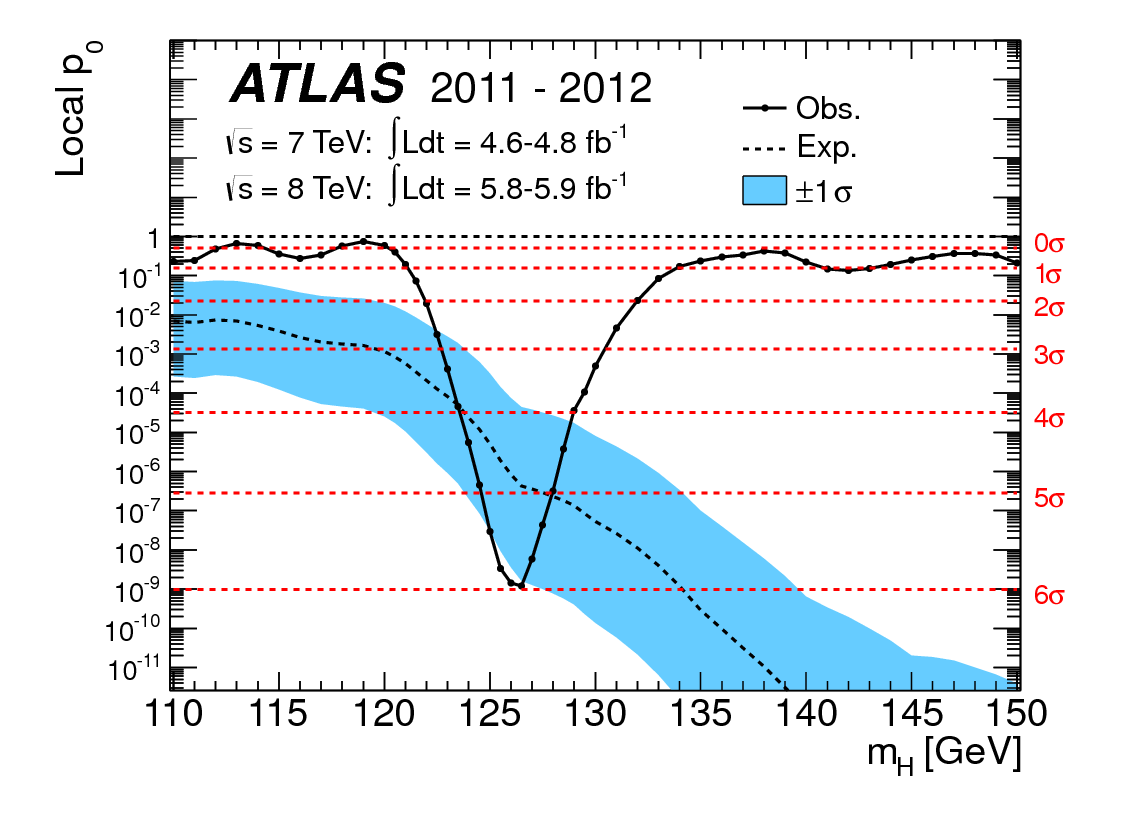
\includegraphics[keepaspectratio,alt={Локальная статистическая значимость в результате ATLAS}]{chapters/../assets/figures/Atlas_pvalue.png}}

\end{center}

\BookInlineFigureCaption{Локальная статистическая значимость в результате ATLAS}

\end{bookgalleryitem}

\begin{bookgalleryitem}

\begin{center}

\pandocbounded{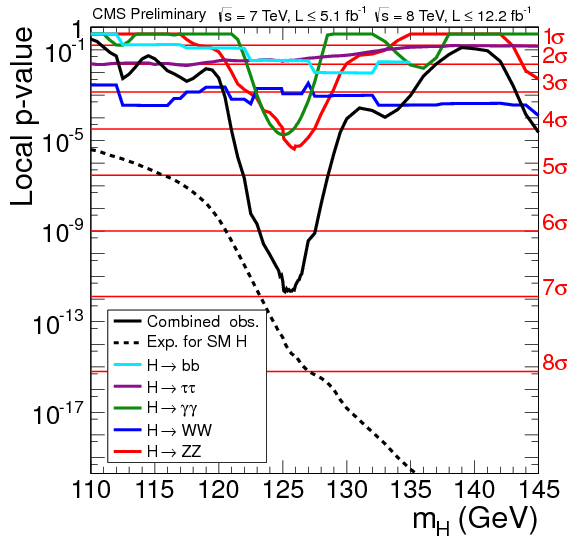
\includegraphics[keepaspectratio,alt={Локальная статистическая значимость в результате CMS}]{chapters/../assets/figures/CMS_pvalue.png}}

\end{center}

\BookInlineFigureCaption{Локальная статистическая значимость в результате CMS}

\end{bookgalleryitem}

За такими графиками стоят фоновая гипотеза, статистика теста,
\(p\)-value, преобразование вероятности в число стандартных отклонений и
учёт области поиска.

\subsection{Измерение и исключение в Daya
Bay}\label{ux438ux437ux43cux435ux440ux435ux43dux438ux435-ux438-ux438ux441ux43aux43bux44eux447ux435ux43dux438ux435-ux432-daya-bay}

Один эксперимент может как измерять параметр, так и исключать область
возможных значений.

\begin{bookgalleryitem}

\begin{center}

\pandocbounded{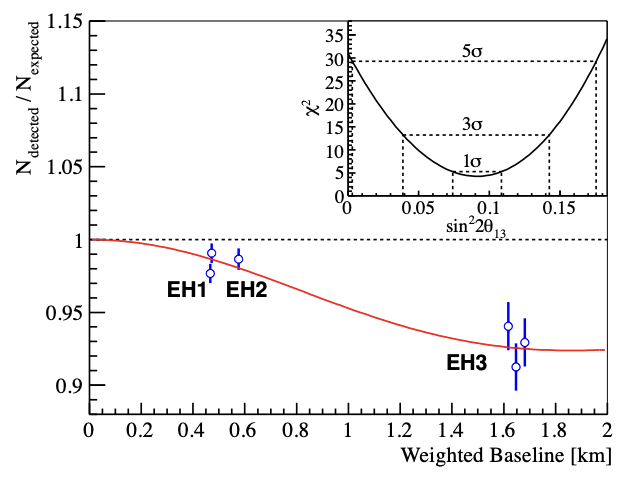
\includegraphics[keepaspectratio,alt={Измерение ненулевого угла смешивания \textbackslash theta\_\{13\}}]{chapters/../assets/figures/DayaBayTheta13.png}}

\end{center}

\BookInlineFigureCaption{Измерение ненулевого угла смешивания \(\theta_{13}\)}

\end{bookgalleryitem}

\begin{bookgalleryitem}

\begin{center}

\pandocbounded{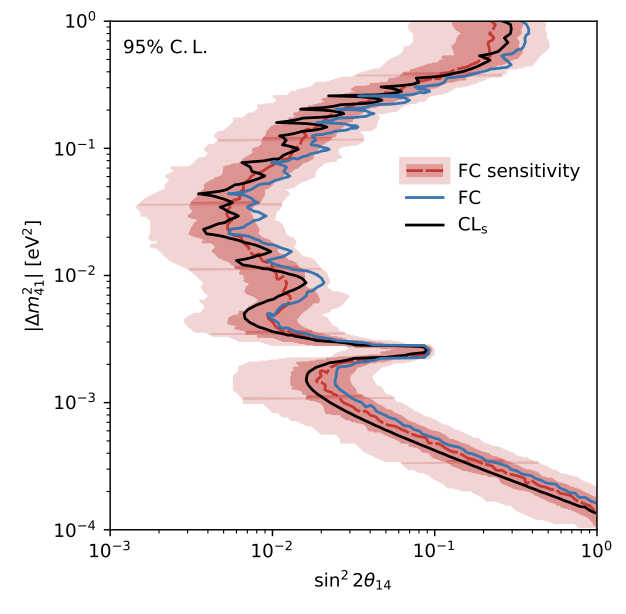
\includegraphics[keepaspectratio,alt={Исключение области параметров стерильных нейтрино}]{chapters/../assets/figures/DBSterile.png}}

\end{center}

\BookInlineFigureCaption{Исключение области параметров стерильных нейтрино}

\end{bookgalleryitem}

В первом случае нужен best fit и неопределённость измерения. Во втором
--- процедура построения границы исключения. В обоих случаях одного
визуального сравнения кривых с точками недостаточно.

\section{Что скрыто в
графиках}\label{ux447ux442ux43e-ux441ux43aux440ux44bux442ux43e-ux432-ux433ux440ux430ux444ux438ux43aux430ux445}

Практически любой законченный физический результат опирается на один и
тот же набор идей:

\begin{itemize}
\tightlist
\item
  случайные флуктуации и распределения вероятности;
\item
  функция правдоподобия или \(\chi^2\);
\item
  оценка параметров и best fit;
\item
  доверительные интервалы и контуры;
\item
  статистическая значимость и \(p\)-value;
\item
  систематические неопределённости и корреляции;
\item
  nuisance-параметры и профилирование;
\item
  верхние пределы и области исключения.
\end{itemize}

Далее эти понятия будут вводиться по одному. Но уже сейчас полезно
увидеть весь процесс на простейшем примере.

\section{Первый фит: ширина
гауссианы}\label{ux43fux435ux440ux432ux44bux439-ux444ux438ux442-ux448ux438ux440ux438ux43dux430-ux433ux430ux443ux441ux441ux438ux430ux43dux44b}

Предположим, что экспериментальные события описываются гауссовым
распределением с известным центром \(x_0=0\) и неизвестной шириной
\(\sigma\):

\[f(x;\sigma)
=
\frac{1}{\sqrt{2\pi}\sigma}
\exp\!\left(-\frac{x^2}{2\sigma^2}\right).\]

Сгенерируем псевдоданные при некотором скрытом значении
\(\sigma_{\mathrm{true}}\). Затем переберём пробные значения \(\sigma\)
и сравним ожидаемое число событий \(\mu_i(\sigma)\) с наблюдаемым
\(n_i\) в каждом интервале.

Для сравнения используем пуассоновский deviance:

\[\chi^2(\sigma)
=
2\sum_i
\left[
\mu_i(\sigma)-n_i
+n_i\ln\frac{n_i}{\mu_i(\sigma)}
\right],\]

где для пустого интервала вклад с логарифмом принимается равным нулю.
Значение \(\widehat{\sigma}\), минимизирующее \(\chi^2(\sigma)\),
является best fit.

\begin{bookapplet}[Интерактив: найдите ширину распределения]

\end{bookapplet}

\begin{figure}[H]

{\centering \pandocbounded{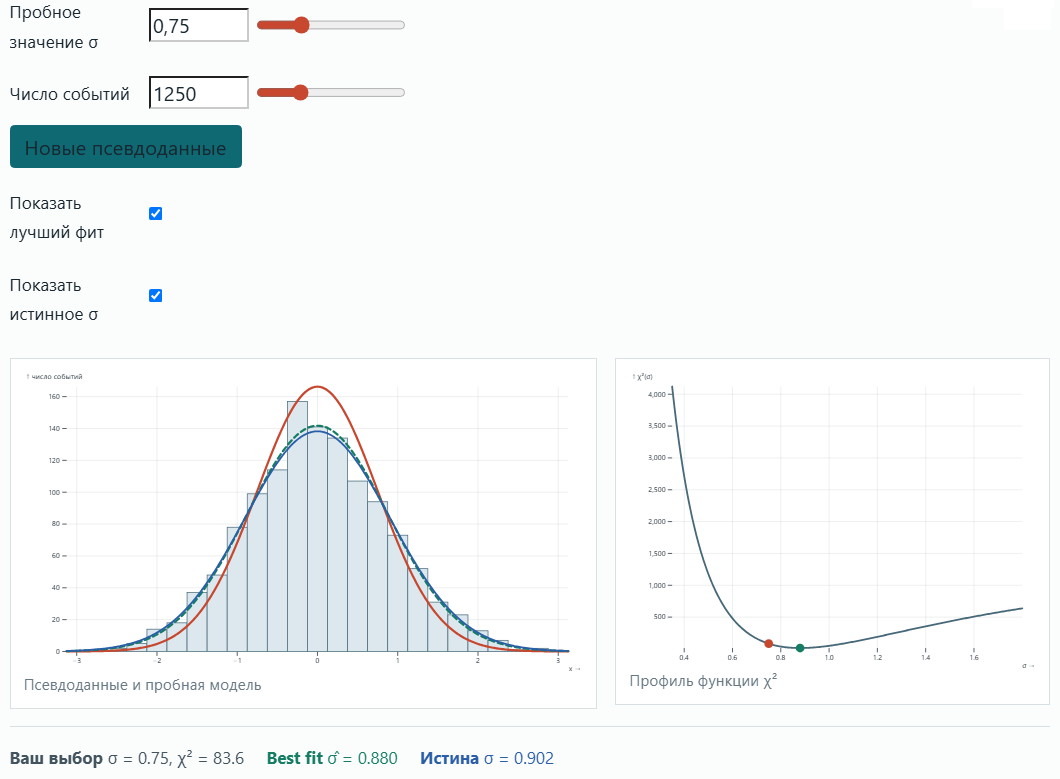
\includegraphics[keepaspectratio]{chapters/../assets/figures/distribution_width.png}}

}

\caption{При одном слагаемом характеристическая функция равномерного
распределения ещё заметно отличается от Гуасса. Статическая версия
интерактивного графика из лекции.}

\end{figure}%

Интерактив показывает несколько общих принципов.

\begin{enumerate}
\def\labelenumi{\arabic{enumi}.}
\tightlist
\item
  Одни и те же данные допускают множество моделей, но согласуются с ними
  по-разному.
\item
  Визуальное совпадение полезно, однако численный критерий делает
  сравнение воспроизводимым.
\item
  Best fit не обязан совпадать с истинным параметром: оценка флуктуирует
  вместе с данными.
\item
  При увеличении числа событий профиль становится уже --- данные точнее
  ограничивают \(\sigma\).
\end{enumerate}

\begin{bookchaptersummary}[Итоги главы]

\begin{itemize}
\tightlist
\item
  Статистическая модель связывает теоретическое предсказание и
  наблюдаемые данные.
\item
  Физический результат всегда зависит не только от данных, но и от
  выбранной процедуры анализа.
\item
  Частотный и байесовский подходы по-разному интерпретируют вероятность.
\item
  Параметр \(\theta\) и его оценка \(\widehat{\theta}\) --- разные
  объекты.
\item
  Даже простейший фит уже содержит данные, модель, функцию сравнения и
  процедуру оценки параметра.
\end{itemize}

\end{bookchaptersummary}

\section{Что
дальше}\label{ux447ux442ux43e-ux434ux430ux43bux44cux448ux435}

Следующая глава вводит случайные величины, математическое ожидание и
моменты --- основные строительные блоки вероятностных моделей.

\begin{booknextchapter}

\href{01_random_distributions.qmd}{Перейти к главе «Случайные величины,
распределения, моменты»}

\end{booknextchapter}

\chapter{Случайные величины, распределения,
моменты}\label{ux441ux43bux443ux447ux430ux439ux43dux44bux435-ux432ux435ux43bux438ux447ux438ux43dux44b-ux440ux430ux441ux43fux440ux435ux434ux435ux43bux435ux43dux438ux44f-ux43cux43eux43cux435ux43dux442ux44b}

\begin{bookchapteropening}[Главная мысль]

Флуктуации данных в эксперименте носят вероятностный характер. В
зависимости от физики задачи подбирается подходящее распределение.

\end{bookchapteropening}

\section{План
главы}\label{ux43fux43bux430ux43d-ux433ux43bux430ux432ux44b}

\begin{itemize}
\tightlist
\item
  Случайность и случайные величины
\item
  Средние, дисперсии и моменты
\item
  Базовые распределения
\item
  Счёт успехов: биномиальная модель
\item
  Счёт редких событий: пуассоновская модель
\item
  Непрерывные ошибки: нормальная модель
\item
  Резюме
\end{itemize}

\section{Случайность и случайные
величины}\label{ux441ux43bux443ux447ux430ux439ux43dux43eux441ux442ux44c-ux438-ux441ux43bux443ux447ux430ux439ux43dux44bux435-ux432ux435ux43bux438ux447ux438ux43dux44b}

{\def\LTcaptype{none} % do not increment counter
\begin{longtable}[]{@{}
  >{\centering\arraybackslash}p{(\linewidth - 4\tabcolsep) * \real{0.4909}}
  >{\centering\arraybackslash}p{(\linewidth - 4\tabcolsep) * \real{0.1636}}
  >{\centering\arraybackslash}p{(\linewidth - 4\tabcolsep) * \real{0.3364}}@{}}
\toprule\noalign{}
\endhead
\bottomrule\noalign{}
\endlastfoot
& \textbf{Случайность} & \\
\textbf{\emph{Классическая физика}} & & \textbf{\emph{Квантовая
физика}} \\
Случайность возникает из-за неполного знания

начальных условий и большого числа степеней свободы & & Случайность
заложена в саму теорию \\
\end{longtable}
}

Эксперимент наблюдает не «идеальное ожидание» , а конкретную реализацию
со статическими флуктуациями. Поэтому сравнение модели с данными всегда
формулируется на языке вероятности.

\textbf{Случайная величина} \(X\) -- экспериментально измеряемая
величина, которая не может быть предсказана до проведения эксперимента.

\textbf{Дискретная} \(X\) описывается \textbf{\emph{функцией вероятности
(PMF -- probability mass function):}}
\[p_k=P(X=x_k), \quad \sum_k p_k=1.\]

\textbf{Непрерывная} \(X\) --- \textbf{\emph{плотностью вероятности}}
\textbf{\emph{(PDF -- probability density function):}}
\[P(x\leq X<x+dx)=f(x)dx, \quad \int_{-\infty}^{+\infty}f(x)dx=1.\] В
обеих записях последние выражения являются соответсвующими условиями
нормировки.

\subsection{Кумулятивная функция распределения
(CDF)}\label{ux43aux443ux43cux443ux43bux44fux442ux438ux432ux43dux430ux44f-ux444ux443ux43dux43aux446ux438ux44f-ux440ux430ux441ux43fux440ux435ux434ux435ux43bux435ux43dux438ux44f-cdf}

Для непрерывной \(X\): \[F(a)=P(X<a)=\int_{-\infty}^a f(x)dx.\] С
математической точки зрения, CDF отражает вероятность того, что \(X<a.\)
\(F(a)\) монотонно возрастает от 0 до 1 при изменении
\(a \in (-\infty,\infty)\). Заметим, что для непрерывных распределений
справедливо следующее свойство: \[F'(a)=f(a).\] При помощи кумулятивной
функции распределения легко вычислить \textbf{\emph{вероятность попасть
в интервал}} \([a,b):\) \[P(a\leq X<b)=F(b)-F(a).\]

\section{Средние, дисперсии и
моменты}\label{ux441ux440ux435ux434ux43dux438ux435-ux434ux438ux441ux43fux435ux440ux441ux438ux438-ux438-ux43cux43eux43cux435ux43dux442ux44b}

\subsection{Моменты
распределения}\label{ux43cux43eux43cux435ux43dux442ux44b-ux440ux430ux441ux43fux440ux435ux434ux435ux43bux435ux43dux438ux44f}

\textbf{\emph{Момент функции}}:
\[\langle x^n\rangle=\mathbb{E}[X^n]=\int_{-\infty}^\infty x^nf(x)dx.\]
Если известны все моменты \(\langle x^n\rangle\), то можно восстановить
\(f(x)\), но это распространяется не на все функции.

\subsection{Практически важные
моменты}\label{ux43fux440ux430ux43aux442ux438ux447ux435ux441ux43aux438-ux432ux430ux436ux43dux44bux435-ux43cux43eux43cux435ux43dux442ux44b}

{\def\LTcaptype{none} % do not increment counter
\begin{longtable}[]{@{}
  >{\centering\arraybackslash}p{(\linewidth - 2\tabcolsep) * \real{0.1465}}
  >{\centering\arraybackslash}p{(\linewidth - 2\tabcolsep) * \real{0.8535}}@{}}
\toprule\noalign{}
\begin{minipage}[b]{\linewidth}\centering
Момент
\end{minipage} & \begin{minipage}[b]{\linewidth}\centering
Формула
\end{minipage} \\
\midrule\noalign{}
\endhead
\bottomrule\noalign{}
\endlastfoot
Среднее &
\(\mu=\langle x\rangle=\mathbb{E}[X]=\int_{-\infty}^{+\infty} xf(x)dx\) \\
Средний квадрат &
\(\langle x^2\rangle=\mathbb{E}[X^2]=\int_{-\infty}^{+\infty} x^2 f(x)dx\) \\
Дисперсия (вариация) &
\(\sigma^2=Var(X)=\mathbb{E}\left[(X-\mu)^2\right]=\mathbb{E}\left[X^2-2\mu X+\mu^2\right]=\langle x^2 \rangle-\langle x\rangle^2\) \\
\end{longtable}
}

\subsection{\texorpdfstring{Моменты распределения произвольной функции
\(g(X)\) случайной
величины}{Моменты распределения произвольной функции g(X) случайной величины}}\label{ux43cux43eux43cux435ux43dux442ux44b-ux440ux430ux441ux43fux440ux435ux434ux435ux43bux435ux43dux438ux44f-ux43fux440ux43eux438ux437ux432ux43eux43bux44cux43dux43eux439-ux444ux443ux43dux43aux446ux438ux438-gx-ux441ux43bux443ux447ux430ux439ux43dux43eux439-ux432ux435ux43bux438ux447ux438ux43dux44b}

{\def\LTcaptype{none} % do not increment counter
\begin{longtable}[]{@{}
  >{\centering\arraybackslash}p{(\linewidth - 2\tabcolsep) * \real{0.1965}}
  >{\centering\arraybackslash}p{(\linewidth - 2\tabcolsep) * \real{0.8035}}@{}}
\toprule\noalign{}
\begin{minipage}[b]{\linewidth}\centering
Момент
\end{minipage} & \begin{minipage}[b]{\linewidth}\centering
Формула
\end{minipage} \\
\midrule\noalign{}
\endhead
\bottomrule\noalign{}
\endlastfoot
Среднее значение функции \(g(X)\) &
\(\langle g(x)\rangle=\mathbb{E}\left[g(X)\right]=\int_{-\infty}^{+\infty} g(x)f(x)dx\) \\
Вариация функции \(g(X)\) &
\(Var(g(X))=\mathbb{E}\left[(g(X)-\langle g(X)\rangle)^2\right]= \int_{-\infty}^\infty \left(g(x)-\langle g(x)\rangle\right)^2 f(x) dx\) \\
\end{longtable}
}

\section{Базовые
распределения}\label{ux431ux430ux437ux43eux432ux44bux435-ux440ux430ux441ux43fux440ux435ux434ux435ux43bux435ux43dux438ux44f}

В рамках данной главы мы рассмотрим три важных примера:

\begin{itemize}
\item
  Биномиальное распределение
\item
  Распределение Пуассона
\item
  Нормальное (гауссово) распределение
\end{itemize}

\section{Счёт успехов: биномиальная
модель}\label{ux441ux447ux451ux442-ux443ux441ux43fux435ux445ux43eux432-ux431ux438ux43dux43eux43cux438ux430ux43bux44cux43dux430ux44f-ux43cux43eux434ux435ux43bux44c}

\begin{booknote}

Если в \(n\) независимых испытаниях вероятность успеха равна \(p\), то
\[P(K=k)=\begin{pmatrix} n\\k\end{pmatrix}p^k(1-p)^{n-k}, \quad k=0,\dots,n,\]
где \[\begin{pmatrix} n\\k\end{pmatrix}=\frac{n!}{k!(n-k)!}\] это число
способов выбрать \(k\) успехов среди \(n\) испытаний.

\end{booknote}

\subsection{Пример биномиального
распределения}\label{ux43fux440ux438ux43cux435ux440-ux431ux438ux43dux43eux43cux438ux430ux43bux44cux43dux43eux433ux43e-ux440ux430ux441ux43fux440ux435ux434ux435ux43bux435ux43dux438ux44f}

Пронаблюдаем \(n\) распадов \(W^{\pm}\). Число распадов \(W\to\mu\nu\):
\[k\sim\mathrm{Bin}(n,p),\] где \(p\) --- вероятность такого распада.
Построим на одних осях три случая: \(n=5,20,100\) при \(p=0.3\).

\begin{Shaded}
\begin{Highlighting}[]
\ImportTok{from}\NormalTok{ math }\ImportTok{import}\NormalTok{ comb}
\ImportTok{import}\NormalTok{ numpy }\ImportTok{as}\NormalTok{ np}

\NormalTok{p }\OperatorTok{=} \FloatTok{0.3}
\ControlFlowTok{for}\NormalTok{ n }\KeywordTok{in}\NormalTok{ [}\DecValTok{5}\NormalTok{, }\DecValTok{20}\NormalTok{, }\DecValTok{100}\NormalTok{]:}
\NormalTok{    k }\OperatorTok{=}\NormalTok{ np.arange(n }\OperatorTok{+} \DecValTok{1}\NormalTok{)}
\NormalTok{    pmf }\OperatorTok{=}\NormalTok{ np.array([comb(n, i) }\OperatorTok{*}\NormalTok{ p}\OperatorTok{**}\NormalTok{i }\OperatorTok{*}\NormalTok{ (}\DecValTok{1}\OperatorTok{{-}}\NormalTok{p)}\OperatorTok{**}\NormalTok{(n}\OperatorTok{{-}}\NormalTok{i) }\ControlFlowTok{for}\NormalTok{ i }\KeywordTok{in}\NormalTok{ k])}
\end{Highlighting}
\end{Shaded}

\begin{bookfigurepanel}

\begin{center}

\pandocbounded{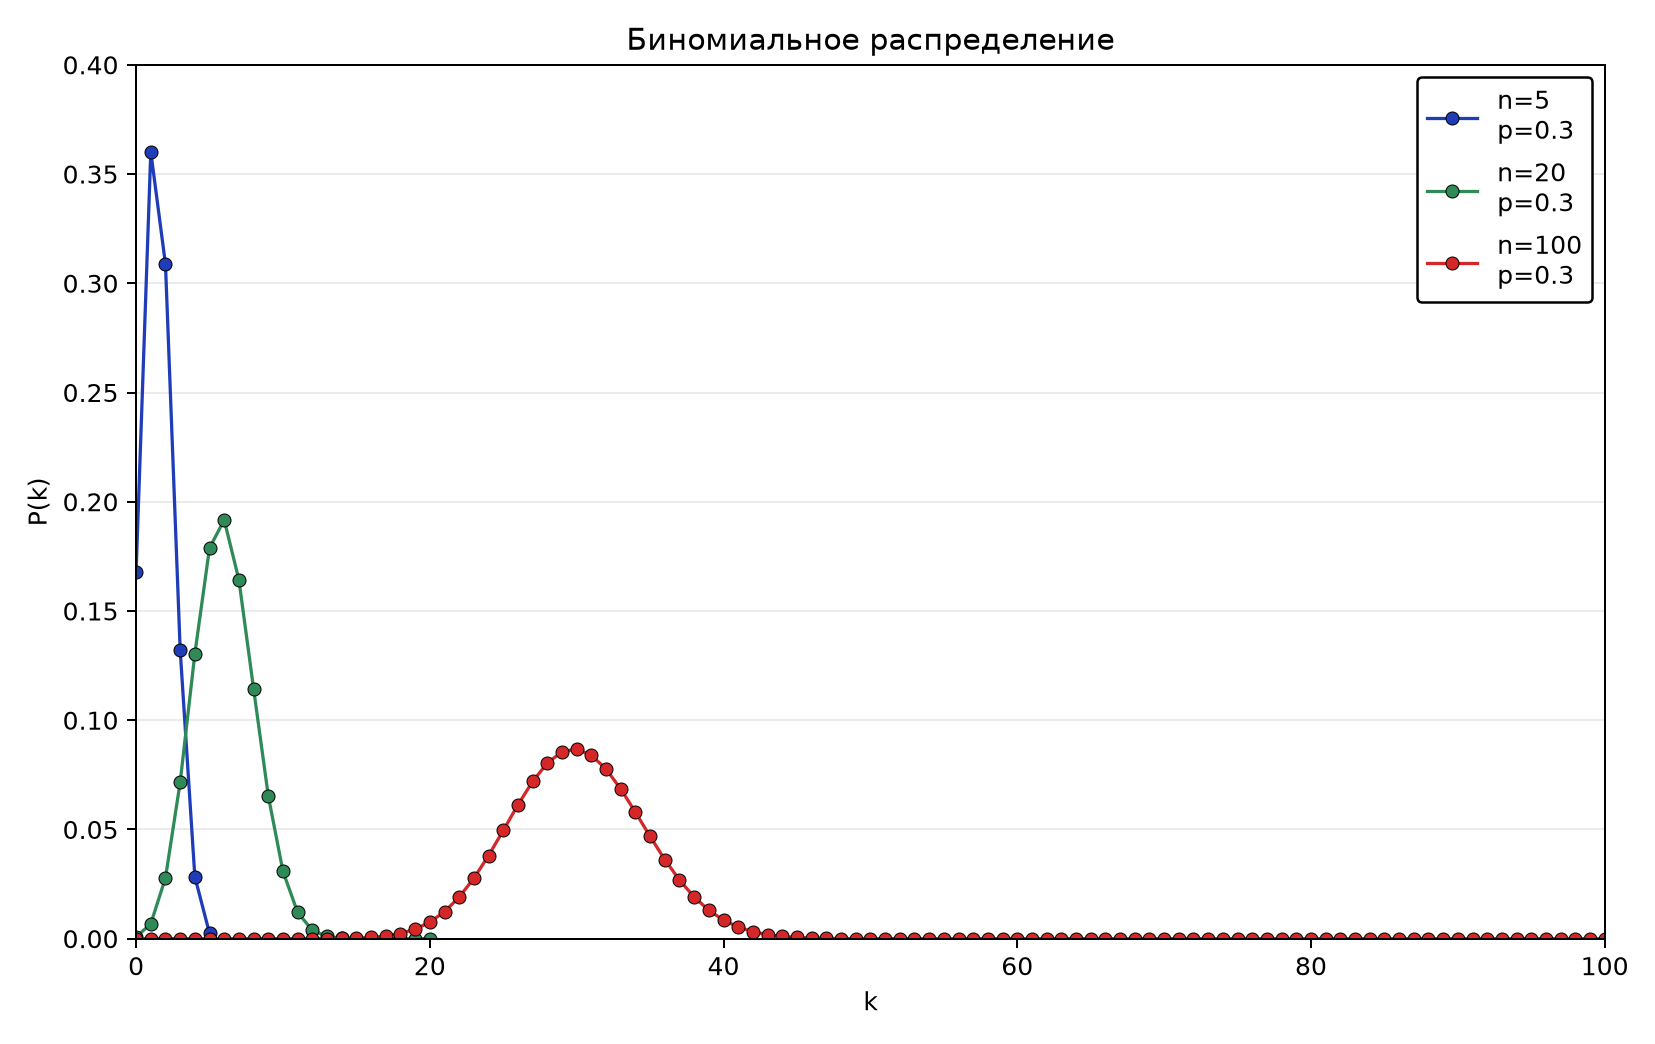
\includegraphics[keepaspectratio,alt={Примеры биномиального распределения}]{chapters/../assets/figures/binomial_pmf_profiles.png}}

\end{center}

\BookInlineFigureCaption{Примеры биномиального распределения}

Обратите внимание, что с увеличением \(n\) биномиальное распределение
переходит в распределение Гаусса (красная кривая).

\end{bookfigurepanel}

\subsection{Моменты биномиального
распределения}\label{ux43cux43eux43cux435ux43dux442ux44b-ux431ux438ux43dux43eux43cux438ux430ux43bux44cux43dux43eux433ux43e-ux440ux430ux441ux43fux440ux435ux434ux435ux43bux435ux43dux438ux44f}

\begin{itemize}
\item
  \textbf{Математическое ожидание:} \(\mathbb{E}[K]=np\)
\item
  \textbf{Дисперсия:} \(Var(K)=np(1-p)\)
\item
  \textbf{Пример:} число распадов нужного канала при фиксированном числе
  родительских частиц
\end{itemize}

\begin{bookderivation}

\subsubsection{\texorpdfstring{\textbf{Вывод}
\(\mathbb{E}[K]\)}{Вывод \textbackslash mathbb\{E\}{[}K{]}}}\label{ux432ux44bux432ux43eux434-mathbbek}

По определению:
\[\mathbb{E}[K]=\sum_{k=0}^n kP(K=k)=\sum_{k=0}^n k \begin{pmatrix} n\\k\end{pmatrix} p^k(1-p)^{n-k}.\]
Используя тождество:
\[k \begin{pmatrix} n\\k\end{pmatrix}=k\frac{n!}{k!(n-k)!}=n\frac{(n-1)!}{(k-1)!(n-k)!}=n\begin{pmatrix} n-1\\k-1\end{pmatrix},\]
получим
\[\mathbb{E}[K]=np\sum_{k=1}^n \begin{pmatrix} n-1\\k-1\end{pmatrix}p^{k-1}(1-p)^{n-k}.\]
Положим \(j=k-1\):
\[\mathbb{E}[K]=np\sum_{j=0}^{n-1} \begin{pmatrix} n-1\\j\end{pmatrix}p^{j}(1-p)^{(n-1)-j},\]
тогда по биному Ньютона:
\[\sum_{j=0}^{n-1} \begin{pmatrix} n-1\\j\end{pmatrix}p^{j}(1-p)^{(n-1)-j}=(p+(1-p))^{n-1}=1.\]
Итог: \[\mathbb{E}[K]=np. \quad \blacksquare\]

\end{bookderivation}

\begin{bookderivation}

\subsubsection{\texorpdfstring{\textbf{Вывод}
\(Var(K)\)}{Вывод Var(K)}}\label{ux432ux44bux432ux43eux434-vark}

Начнем со второго факториального момента:
\[\mathbb{E}[K(K-1)]=\sum_{k=0}^n k(k-1) \begin{pmatrix} n\\k\end{pmatrix} p^k(1-p)^{n-k}.\]
Используя тождество:
\[k(k-1) \begin{pmatrix} n\\k\end{pmatrix}=k(k-1)\frac{n!}{k!(n-k)!}=n(n-1)\frac{(n-2)!}{(k-2)!(n-k)!}=n(n-1)\begin{pmatrix} n-2\\k-2\end{pmatrix},\]
получим
\[\mathbb{E}[K(K-1)]=n(n-1)p^2\sum_{k=2}^n \begin{pmatrix} n-2\\k-2\end{pmatrix} p^{k-2}(1-p)^{n-k}=n(n-1)p^2.\]
Воспользуемся разложением \(K^2\): \[K^2=K(K-1)+K,\] тогда
\[\mathbb{E}[K^2]=\mathbb{E}[K(K-1)]+\mathbb{E}[K]=n(n-1)p^2+np.\] Таким
образом, вариацию \(Var(K)\) можно записать в виде:
\[Var(K)=\mathbb{E}[K^2]-\mathbb{E}[K]^2=\left(n(n-1)p^2+np\right)-(np)^2.\]
Итог: \[Var(K)=np(1-p). \quad \blacksquare\]

\end{bookderivation}

\section{Счёт редких событий: пуассоновская
модель}\label{ux441ux447ux451ux442-ux440ux435ux434ux43aux438ux445-ux441ux43eux431ux44bux442ux438ux439-ux43fux443ux430ux441ux441ux43eux43dux43eux432ux441ux43aux430ux44f-ux43cux43eux434ux435ux43bux44c}

\begin{booknote}

\textbf{Распределение Пуассона} моделирует число событий в фиксированном
интервале времени или пространства при постоянной средней интенсивности
\(λ\) и независимых событиях.

Вероятность наблюдения~\(N=k\)~событий при среднем числе событий \(λ\):
\[P(N=k)=\frac{\lambda^k e^{-\lambda}}{k!}, \quad k=0,1,2,\dots\]
Пример: число распадов радиоактивного источника за 1 минуту.

\end{booknote}

\subsection{Пример распределения
Пуассона}\label{ux43fux440ux438ux43cux435ux440-ux440ux430ux441ux43fux440ux435ux434ux435ux43bux435ux43dux438ux44f-ux43fux443ux430ux441ux441ux43eux43dux430}

Посчитаем число событий \(N\) за фиксированное время. Если среднее число
событий равно \(\lambda\), то \[N\sim \mathrm{Pois}(\lambda).\] Построим
на одних осях три случая: \(\lambda=1,4,10\).

\begin{Shaded}
\begin{Highlighting}[]
\ImportTok{from}\NormalTok{ math }\ImportTok{import}\NormalTok{ factorial}
\ImportTok{import}\NormalTok{ numpy }\ImportTok{as}\NormalTok{ np}

\ControlFlowTok{for}\NormalTok{ lam }\KeywordTok{in}\NormalTok{ [}\DecValTok{1}\NormalTok{, }\DecValTok{4}\NormalTok{, }\DecValTok{10}\NormalTok{]:}
\NormalTok{    k }\OperatorTok{=}\NormalTok{ np.arange(}\DecValTok{26}\NormalTok{)}
\NormalTok{    pmf }\OperatorTok{=}\NormalTok{ np.exp(}\OperatorTok{{-}}\NormalTok{lam) }\OperatorTok{*}\NormalTok{ lam}\OperatorTok{**}\NormalTok{k }\OperatorTok{/}\NormalTok{ np.array([factorial(i) }\ControlFlowTok{for}\NormalTok{ i }\KeywordTok{in}\NormalTok{ k])}
\end{Highlighting}
\end{Shaded}

\begin{bookfigurepanel}

\begin{center}

\pandocbounded{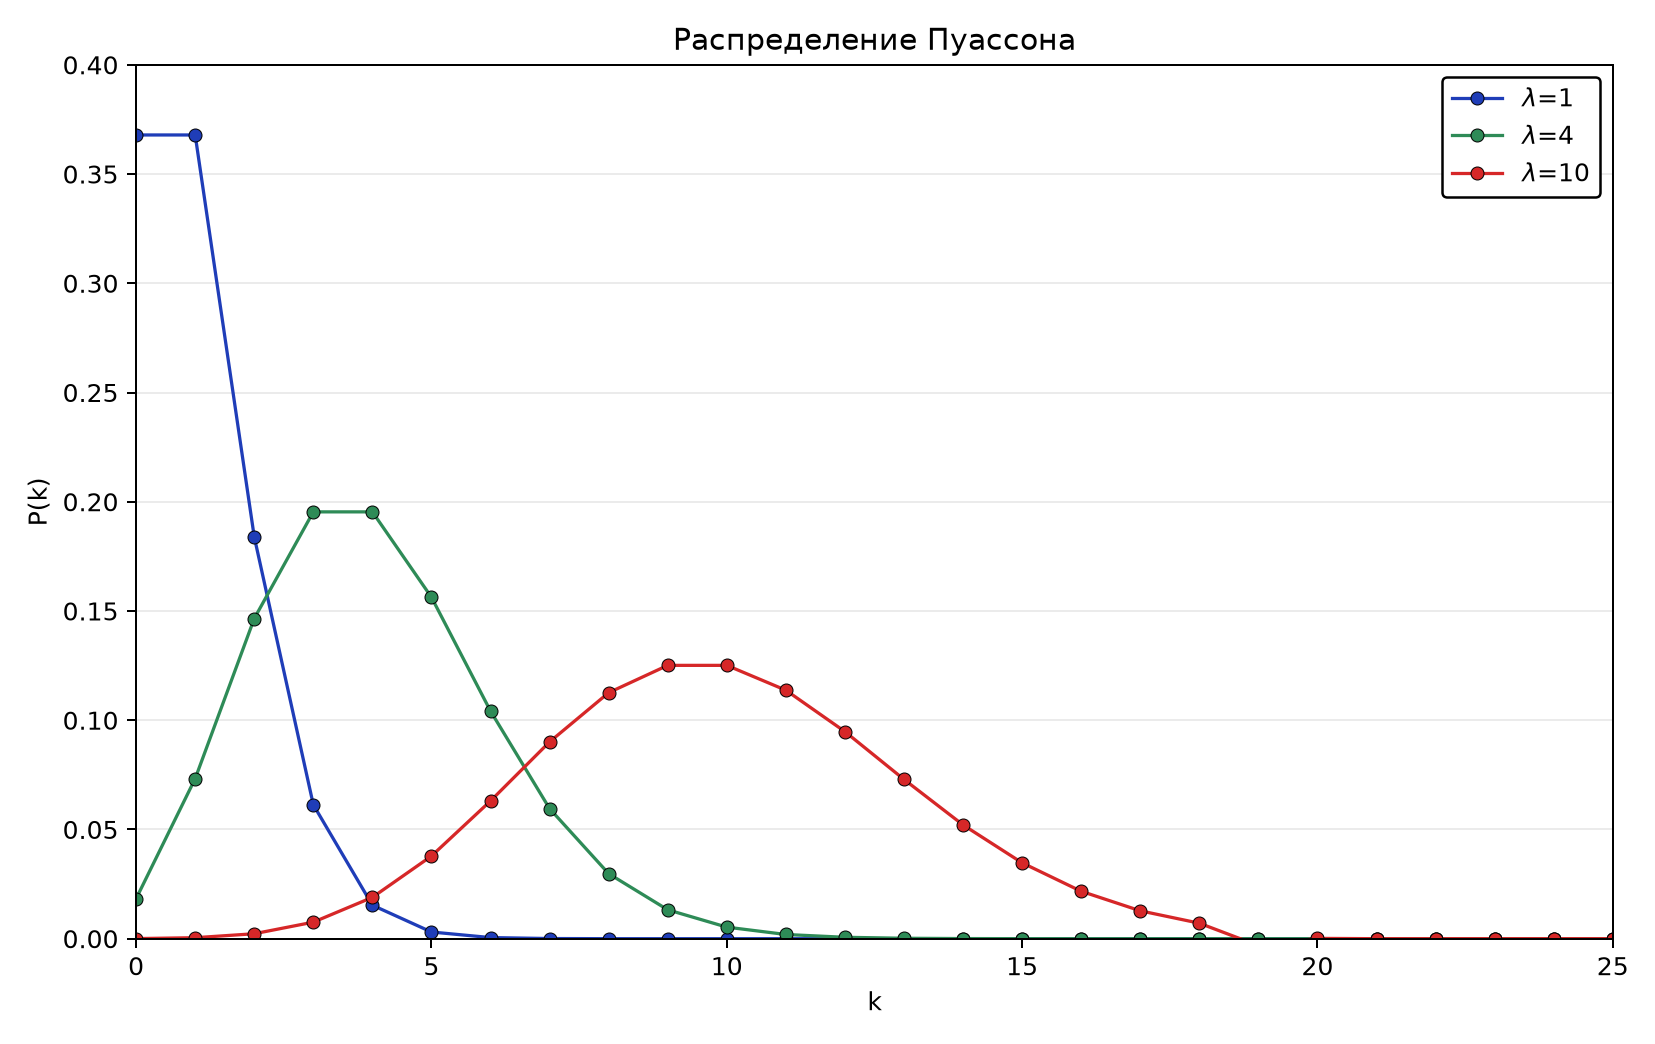
\includegraphics[keepaspectratio,alt={Примеры распределения Пуассона}]{chapters/../assets/figures/poisson_pmf_profiles.png}}

\end{center}

\BookInlineFigureCaption{Примеры распределения Пуассона}

Обратите внимание, что с увеличением \(n\) распределение Пуассона также
стремиться к нормальному распределению (красная кривая).

\end{bookfigurepanel}

\subsection{Моменты распределения
Пуассона}\label{ux43cux43eux43cux435ux43dux442ux44b-ux440ux430ux441ux43fux440ux435ux434ux435ux43bux435ux43dux438ux44f-ux43fux443ux430ux441ux441ux43eux43dux430}

\begin{itemize}
\item
  \textbf{Математическое ожидание:} \(\mathbb{E}[K]=\lambda\)
\item
  \textbf{Дисперсия:} \(Var(K)=\lambda\)
\end{itemize}

\begin{bookderivation}

\subsubsection{\texorpdfstring{\textbf{Вывод}
\(\mathbb{E}[N]\)}{Вывод \textbackslash mathbb\{E\}{[}N{]}}}\label{ux432ux44bux432ux43eux434-mathbben}

По определению:
\[\mathbb{E}[N]=\sum_{k=0}^\infty k\frac{\lambda^k e^{-\lambda}}{k!}.\]
Вынесем множитель за сумму:
\[\mathbb{E}[N]=\lambda e^{-\lambda}\sum_{k=1}^\infty \frac{\lambda^{k-1} }{(k-1)!}.\]
Сдвинем индекс \(j=k-1\), не забыв разложение экспоненты в ряд Тейлора :
\[\mathbb{E}[N]=\lambda e^{-\lambda}\sum_{j=0}^\infty \frac{\lambda^{j} }{j!}=\lambda e^{-\lambda}e^{\lambda}=\lambda.\]
Итог: \[\mathbb{E}[N]=\lambda. \quad \blacksquare\]

\end{bookderivation}

\begin{bookderivation}

\subsubsection{\texorpdfstring{\textbf{Вывод}
\(Var(N)\)}{Вывод Var(N)}}\label{ux432ux44bux432ux43eux434-varn}

Воспользуемся уже знакомым вторым факториальным моментом:
\[\mathbb{E}[N(N-1)]=\sum_{k=0}^\infty k(k-1)\frac{\lambda^k e^{-\lambda}}{k!}.\]
Поскольку \[\frac{k(k-1)}{k!}=\frac{1}{(k-2)!},\] то можно преобразовать
выражение для момента:
\[\mathbb{E}[N(N-1)]=\lambda^2 e^{-\lambda}\sum_{k=2}^\infty \frac{\lambda^{k-2} }{(k-2)!}=\lambda^2 e^{-\lambda}\sum_{j=0}^\infty \frac{\lambda^{j} }{j!}=\lambda^2.\]
Используя связь: \[N^2=N(N-1)+N,\] получим
\[\mathbb{E}[N^2]=\mathbb{E}[N(N-1)]+\mathbb{E}[N]=\lambda^2+\lambda.\]
Таким образом, вариацию \(Var(N)\) можно записать в виде:
\[Var(N)=\mathbb{E}[N^2]-\mathbb{E}[N]^2=(\lambda^2+\lambda)-\lambda^2=\lambda.\]
Итог: \[Var(N)=\lambda. \quad \blacksquare\]

\end{bookderivation}

\section{Непрерывные ошибки: нормальная
модель}\label{ux43dux435ux43fux440ux435ux440ux44bux432ux43dux44bux435-ux43eux448ux438ux431ux43aux438-ux43dux43eux440ux43cux430ux43bux44cux43dux430ux44f-ux43cux43eux434ux435ux43bux44c}

\begin{booknote}

\subsection{Нормальное (гауссово)
распределение}\label{ux43dux43eux440ux43cux430ux43bux44cux43dux43eux435-ux433ux430ux443ux441ux441ux43eux432ux43e-ux440ux430ux441ux43fux440ux435ux434ux435ux43bux435ux43dux438ux435}

\[f(x;\mu,\sigma)=\frac{1}{\sigma (2\pi)^{1/2}}\exp\left[-\frac{(x-\mu)^2}{2\sigma^2}\right],\]

где \(\mu\) -- среднее значение, \(\sigma\) - дисперсия случайной
величины. Оно часто представимо в виде суммы многих малых независимых
вкладов.

\end{booknote}

Так почему же распределение «нормальное»?

\begin{quote}
Много лет назад я назвал кривую Лапласа-Гаусса нормальной кривой. Это
название, избегая международного спора о приоритете, имеет недостаток:
оно заставляет думать, что все прочие распределения частот в том или
ином смысле «ненормальны».

К. Пирсон (1920)
\end{quote}

\subsection{Пример нормального
распределения}\label{ux43fux440ux438ux43cux435ux440-ux43dux43eux440ux43cux430ux43bux44cux43dux43eux433ux43e-ux440ux430ux441ux43fux440ux435ux434ux435ux43bux435ux43dux438ux44f}

Параметр \(\mu\) задаёт среднее значение, \(\sigma\) --- ширину разброса
величины. Построим на одних осях три случая:
\((\mu,\sigma)=(0,1),(0,2),(2,1)\).

\begin{Shaded}
\begin{Highlighting}[]
\ImportTok{import}\NormalTok{ numpy }\ImportTok{as}\NormalTok{ np}

\NormalTok{x }\OperatorTok{=}\NormalTok{ np.linspace(}\OperatorTok{{-}}\DecValTok{6}\NormalTok{, }\DecValTok{6}\NormalTok{, }\DecValTok{400}\NormalTok{)}
\ControlFlowTok{for}\NormalTok{ mu, sigma }\KeywordTok{in}\NormalTok{ [(}\DecValTok{0}\NormalTok{, }\DecValTok{1}\NormalTok{), (}\DecValTok{0}\NormalTok{, }\DecValTok{2}\NormalTok{), (}\DecValTok{2}\NormalTok{, }\DecValTok{1}\NormalTok{)]:}
\NormalTok{    pdf }\OperatorTok{=}\NormalTok{ np.exp(}\OperatorTok{{-}}\FloatTok{0.5}\OperatorTok{*}\NormalTok{((x}\OperatorTok{{-}}\NormalTok{mu)}\OperatorTok{/}\NormalTok{sigma)}\OperatorTok{**}\DecValTok{2}\NormalTok{)}\OperatorTok{/}\NormalTok{(sigma}\OperatorTok{*}\NormalTok{np.sqrt(}\DecValTok{2}\OperatorTok{*}\NormalTok{np.pi))}
\end{Highlighting}
\end{Shaded}

\begin{bookfigurepanel}

\begin{center}

\pandocbounded{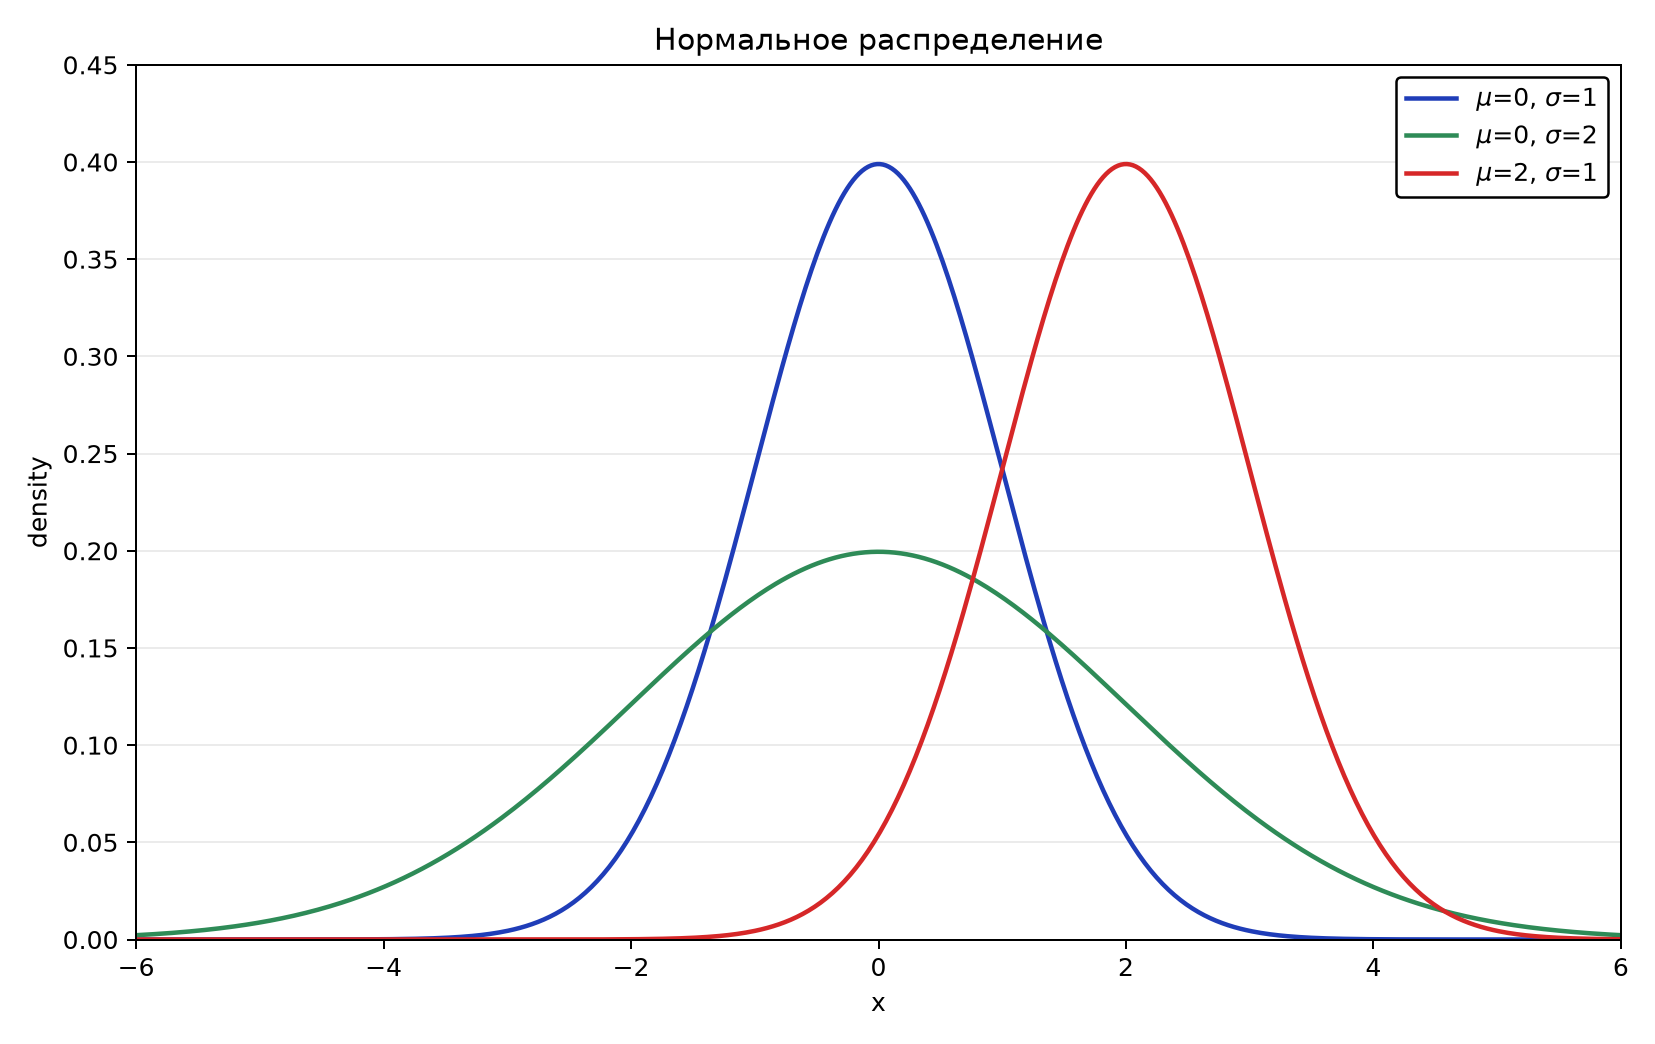
\includegraphics[keepaspectratio,alt={Примеры распределения Гаусса}]{chapters/../assets/figures/normal_density_profiles.png}}

\end{center}

\BookInlineFigureCaption{Примеры распределения Гаусса}

Из графика видно, что чем меньше \(\sigma\), тем уже распределение.

\end{bookfigurepanel}

\subsection{Моменты распределения
Гуасса}\label{ux43cux43eux43cux435ux43dux442ux44b-ux440ux430ux441ux43fux440ux435ux434ux435ux43bux435ux43dux438ux44f-ux433ux443ux430ux441ux441ux430}

\begin{itemize}
\item
  \textbf{Математическое ожидание:} \(\mathbb{E}[X]=\mu\)
\item
  \textbf{Дисперсия:} \(Var(X)=\sigma^2\)
\end{itemize}

\begin{bookderivation}

\subsubsection{\texorpdfstring{\textbf{Вывод}
\(\mathbb{E}[X]\)}{Вывод \textbackslash mathbb\{E\}{[}X{]}}}\label{ux432ux44bux432ux43eux434-mathbbex}

По определению:
\[\mathbb{E}[X]=\int_{-\infty}^\infty x\frac{1}{\sigma (2\pi)^{1/2}}\exp\left[-\frac{(x-\mu)^2}{2\sigma^2}\right]dx.\]
Перейдем к стандартной нормали:~\(z=(x−μ)/σ,~x=μ+σz,~dx=σdz:\)
\[\mathbb{E}[X]=\int_{-\infty}^\infty (\mu+\sigma z)\varphi(z)dz, \quad \varphi(z)=\frac{1}{\sqrt{2\pi}}e^{-z^2/2}.\]
\[\mathbb{E}[X]=\mu\int_{-\infty}^\infty \varphi(z)dz+\sigma\int_{-\infty}^\infty z\varphi(z)dz=\mu\cdot1+\sigma\cdot 0=\mu,\]
так как \(z\varphi(z)\) нечётная функция.

Итог: \[\mathbb{E}[X]=\mu. \quad \blacksquare\]

\end{bookderivation}

\begin{bookderivation}

\subsubsection{\texorpdfstring{\textbf{Вывод}
\(Var(X)\)}{Вывод Var(X)}}\label{ux432ux44bux432ux43eux434-varx}

По определению:
\[Var(X)=\mathbb{E}\left[(X-\mu)^2\right]=\int_{-\infty}^\infty (x-\mu)^2 f(x)dx.\]
Делая замену переменных \(z=(x-\mu)/\sigma,\) получим:
\[Var(X)=\sigma^2\int_{-\infty}^\infty z^2 \varphi(z) dz=\sigma^2 \mathbb{E}\left[Z^2\right], \quad Z\sim N(0,1),\]
где
\[\mathbb{E}\left[Z^2\right]=\int_{-\infty}^\infty z^2 \varphi(z)dz=\left[-z\varphi(z)\right]^{\infty}_{-\infty}+\int_{-\infty}^\infty \varphi(z)dz=1.\]
Итог: \[Var(X)=\sigma^2. \quad \blacksquare\]

\end{bookderivation}

\section{Резюме по
распределениям}\label{ux440ux435ux437ux44eux43cux435-ux43fux43e-ux440ux430ux441ux43fux440ux435ux434ux435ux43bux435ux43dux438ux44fux43c}

{\def\LTcaptype{none} % do not increment counter
\begin{longtable}[]{@{}
  >{\centering\arraybackslash}p{(\linewidth - 6\tabcolsep) * \real{0.1926}}
  >{\centering\arraybackslash}p{(\linewidth - 6\tabcolsep) * \real{0.1037}}
  >{\centering\arraybackslash}p{(\linewidth - 6\tabcolsep) * \real{0.1111}}
  >{\centering\arraybackslash}p{(\linewidth - 6\tabcolsep) * \real{0.5778}}@{}}
\toprule\noalign{}
\begin{minipage}[b]{\linewidth}\centering
Название
\end{minipage} & \begin{minipage}[b]{\linewidth}\centering
Среднее
\end{minipage} & \begin{minipage}[b]{\linewidth}\centering
Дисперсия
\end{minipage} & \begin{minipage}[b]{\linewidth}\centering
Условия применения
\end{minipage} \\
\midrule\noalign{}
\endhead
\bottomrule\noalign{}
\endlastfoot
Биномиальное

\(K\sim Bin(n,p)\) & \(np\) & \(np(1-p)\) & Фиксированное \(n\);
независимые испытания; постоянное \(p\). \\
Пуассон

\(N\sim Pois(\lambda)\) & \(\lambda\) & \(\lambda\) & События в
фиксированном интервале; постоянная интенсивность; независимость. \\
Нормальное

\(X\sim N(\mu,\sigma)\) & \(\mu\) & \(\sigma^2\) & Непрерывные ошибки;
сумма многих малых независимых вкладов \\
\end{longtable}
}

\begin{bookchaptersummary}[Итоги главы]

\begin{itemize}
\tightlist
\item
  Данные в эксперименте флуктуируют, и эти флуктуации нужно описывать
  вероятностно.
\item
  Выбор распределения определяется физикой задачи.
\item
  Среднее и дисперсия --- первые количественные характеристики
  распределения.
\item
  Биномиальное, пуассоновское и нормальное распределения --- базовый
  рабочий набор экспериментатора.
\end{itemize}

\end{bookchaptersummary}

Материалы курса:

\begin{itemize}
\tightlist
\item
  \href{https://neutrinohit.github.io/statistical-analysis-course/ru/slides/01_random_distributions.html}{Слайды
  лекции}
\item
  \href{https://neutrinohit.github.io/statistical-analysis-course/ru/slides/exercises/01_random_distributions_exercises.html}{Задачи}
\end{itemize}

\chapter{Характеристические функции и суммы случайных
величин}\label{ux445ux430ux440ux430ux43aux442ux435ux440ux438ux441ux442ux438ux447ux435ux441ux43aux438ux435-ux444ux443ux43dux43aux446ux438ux438-ux438-ux441ux443ux43cux43cux44b-ux441ux43bux443ux447ux430ux439ux43dux44bux445-ux432ux435ux43bux438ux447ux438ux43d}

\begin{bookchapteropening}[Главная мысль]

При сложении независимых случайных величин их плотности приходится
свёртывать, и прямое вычисление быстро становится громоздким.
Характеристическая функция переводит эту задачу в пространство Фурье,
где свёртка превращается в обычное произведение. Благодаря этому суммы
случайных величин, их моменты и кумулянты можно исследовать гораздо
проще.

\end{bookchapteropening}

\section{План
главы}\label{ux43fux43bux430ux43d-ux433ux43bux430ux432ux44b-1}

\begin{itemize}
\tightlist
\item
  Распределение суммы независимых случайных величин и свёртка
\item
  Пример: распределение Коши
\item
  Характеристическая функция как преобразование Фурье
\item
  Основные свойства характеристической функции
\item
  Суммы независимых случайных величин
\item
  Примеры: Бернулли, Пуассон, Гаусс и Коши
\item
  Моменты как производные характеристической функции
\item
  Кумулянты и их свойства
\item
  Мост к центральной предельной теореме
\item
  Резюме
\end{itemize}

\section{Распределение суммы независимых случайных
величин}\label{ux440ux430ux441ux43fux440ux435ux434ux435ux43bux435ux43dux438ux435-ux441ux443ux43cux43cux44b-ux43dux435ux437ux430ux432ux438ux441ux438ux43cux44bux445-ux441ux43bux443ux447ux430ux439ux43dux44bux445-ux432ux435ux43bux438ux447ux438ux43d}

Пусть \(X\) и \(Y\) -- две независимые случайные величины с известными
плотностями вероятности \(f_X(x)\) и \(f_Y(y)\). Требуется найти
плотность вероятности их суммы \[S=X+Y.\] Подобная задача естественно
возникает, когда эксперимент не различает отдельные вклады, а
регистрирует только их сумму, например, при работе с энерговыделением
или зарядом. Чтобы сумма приняла конкретное значение \(S=s\), нужно
учесть все возможные пары значений \((x,y)\), для которых \[x+y=s.\]
Если выбрать значение \(x\), то второе значение уже определяется
условием суммы: \[y=s-x.\] Поскольку \(X\) и \(Y\) независимы, плотности
для такой пары перемножаются. После этого нужно просуммировать вклады от
всех допустимых \(x\), то есть проинтегрировать по всей области
изменения случайной величины: \[\boxed{
f_S(s)
=
\int_{-\infty}^{+\infty}
f_X(x)f_Y(s-x)\,dx.
}\] Такой интеграл называется \textbf{свёрткой}. Кратко его можно
записать как: \[f_S=f_X*f_Y.\] Звёздочка здесь обозначает не обычное
умножение, а операцию свёртки.

\subsection{Сумма нескольких
величин}\label{ux441ux443ux43cux43cux430-ux43dux435ux441ux43aux43eux43bux44cux43aux438ux445-ux432ux435ux43bux438ux447ux438ux43d}

Для трёх независимых случайных величин \(X\), \(Y\) и \(Z\) задача уже
приводит к двойному интегралу: \[f_S(s)
=
\int_{-\infty}^{+\infty}
\int_{-\infty}^{+\infty}
f_X(x)f_Y(y)f_Z(s-x-y)\,dx\,dy,\] где \[S=X+Y+Z.\] Для суммы
\[S_n=X_1+X_2+\dots+X_n\] получаем последовательную свёртку: \[\boxed{
f_{S_n}=f_{X_1}*f_{X_2}*\cdots*f_{X_n}.
}\] В развёрнутом виде: \[\begin{aligned}
f_{S_n}(s)
={}&
\int_{-\infty}^{+\infty}\cdots
\int_{-\infty}^{+\infty}
f_{X_1}(x_1)f_{X_2}(x_2)\cdots \\
&\qquad\times
f_{X_n}(s-x_1-\cdots-x_{n-1})
\,dx_1\cdots dx_{n-1}.
\end{aligned}\] С ростом числа слагаемых размерность интеграла
возрастает. Именно здесь становится заметна практическая проблема
прямого подхода: даже если такие интегралы возможно вычислить, их
вычисления быстро усложняются.

\section{Пример: распределение
Коши}\label{ux43fux440ux438ux43cux435ux440-ux440ux430ux441ux43fux440ux435ux434ux435ux43bux435ux43dux438ux435-ux43aux43eux448ux438}

В качестве примера рассмотрим распределение Коши с параметрами \(x_0\) и
\(\gamma\): \[\boxed{
f_X(x;x_0,\gamma)
=
\frac{1}
{\pi\gamma\left[1+\left(\frac{x-x_0}{\gamma}\right)^2\right]}.
}\] В физике это распределение также известно как распределение Лоренца
или Брейта--Вигнера. Оно встречается при описании резонансов в физике
частиц, а также спектров излучения в атомной и молекулярной физике.

Стандартное распределение Коши получается при

\[x_0=0,
\qquad
\gamma=1,\] и имеет вид: \[\boxed{
f_X(x)=\frac{1}{\pi(1+x^2)}.
}\]

\begin{booknote}

Запись \[X\sim \mathrm{Cauchy}(0,1)\] означает, что случайная величина
\(X\) \textbf{распределена согласно стандартному распределению Коши}.
Знак \(\sim\) в такой записи не означает «примерно равно».

\end{booknote}

\subsection{Прямая свёртка двух распределений
Коши}\label{ux43fux440ux44fux43cux430ux44f-ux441ux432ux451ux440ux442ux43aux430-ux434ux432ux443ux445-ux440ux430ux441ux43fux440ux435ux434ux435ux43bux435ux43dux438ux439-ux43aux43eux448ux438}

Пусть две независимые случайные величины распределены одинаково:
\[X,Y\sim\mathrm{Cauchy}(0,1),\] то есть
\[f_X(x)=f_Y(x)=\frac{1}{\pi(1+x^2)}.\] Для суммы \[S=X+Y\] прямая
свёртка равна \[\boxed{
f_S(s)
=
\frac{1}{\pi^2}
\int_{-\infty}^{+\infty}
\frac{dx}
{(1+x^2)\left[1+(s-x)^2\right]}.
}\] Уже здесь знаменатель содержит многочлен четвёртой степени по \(x\).
Такой интеграл можно вычислять, например, раскладывая выражение на
простые дроби или применяя теорему о вычетах, но после интегрирования
результат ещё нужно существенно упростить.

Таким образом, даже сумма всего двух достаточно простых распределений
приводит к заметно более громоздкому вычислению. Это и есть основная
мотивация для перехода к характеристическим функциям.

\section{Характеристическая
функция}\label{ux445ux430ux440ux430ux43aux442ux435ux440ux438ux441ux442ux438ux447ux435ux441ux43aux430ux44f-ux444ux443ux43dux43aux446ux438ux44f}

\begin{booknote}

В статистическом анализе \textbf{характеристической функцией} называют
преобразование Фурье распределения. Для случайной величины \(X\) она
определяется как \[\boxed{
\varphi_X(t)
=
\mathbb{E}\!\left[e^{itX}\right].
}\] Для непрерывной случайной величины с плотностью \(f_X(x)\)
математическое ожидание записывается интегралом: \[\boxed{
\varphi_X(t)
=
\int_{-\infty}^{+\infty}
e^{itx}f_X(x)\,dx.
}\] Здесь \(x\) -- переменная интегрирования, а \(t\) -- аргумент
характеристической функции.

\end{booknote}

Если плотность существует, её можно восстановить обратным
преобразованием Фурье: \[\boxed{
f_X(x)
=
\frac{1}{2\pi}
\int_{-\infty}^{+\infty}
e^{-itx}\varphi_X(t)\,dt.
}\] Поэтому характеристическая функция содержит ту же информацию о
случайной величине, что и исходная плотность распределения. Если
известна \(\varphi_X(t)\), можно восстановить \(f_X(x)\) и тем самым
получить исходное распределение.

Главное преимущество для задачи о сумме независимых величин состоит в
том, что \textbf{свёртка плотностей в обычном пространстве превращается
в произведение характеристических функций в пространстве Фурье}.

\section{Сумма двух величин Коши через характеристические
функции}\label{ux441ux443ux43cux43cux430-ux434ux432ux443ux445-ux432ux435ux43bux438ux447ux438ux43d-ux43aux43eux448ux438-ux447ux435ux440ux435ux437-ux445ux430ux440ux430ux43aux442ux435ux440ux438ux441ux442ux438ux447ux435ux441ux43aux438ux435-ux444ux443ux43dux43aux446ux438ux438}

Для стандартного распределения Коши характеристическая функция имеет
особенно простой вид: \[\boxed{
\varphi_X(t)=e^{-|t|}.
}\] Данный Фурье-образ можно самостоятельно получить при помощи теоремы
о вычетах. Рассмотрим снова две независимые величины:
\[X,Y\sim\mathrm{Cauchy}(0,1)\] и их сумму: \[S=X+Y.\] По определению:
\[\varphi_S(t)
=
\mathbb{E}\!\left[e^{it(X+Y)}\right].\] Экспонента от суммы
раскладывается в произведение: \[e^{it(X+Y)}=e^{itX}e^{itY}.\] А
поскольку \(X\) и \(Y\) независимы, математическое ожидание произведения
раскладывается в произведение математических ожиданий: \[\begin{aligned}
\varphi_S(t)
&=
\mathbb{E}\!\left[e^{itX}e^{itY}\right] \\
&=
\mathbb{E}\!\left[e^{itX}\right]
\mathbb{E}\!\left[e^{itY}\right] \\
&=
\varphi_X(t)\varphi_Y(t).
\end{aligned}\] Для стандартных распределений Коши получается:
\[\varphi_S(t)
=
e^{-|t|}e^{-|t|}
=
e^{-2|t|}.\] Но \(e^{-2|t|}\) -- характеристическая функция
распределения Коши с параметрами \(0\) и \(2\). Поэтому \[\boxed{
S=X+Y\sim\mathrm{Cauchy}(0,2).
}\] Тогда плотность суммы можно записать как: \[\boxed{
f_S(s)=\frac{2}{\pi(s^2+4)}.
}\] В итоге, то, что при прямой свёртке требовало вычисления
нетривиального интеграла, в пространстве Фурье свелось к умножению двух
простых функций.

\begin{bookfigurepanel}

\begin{figure}[H]

{\centering \pandocbounded{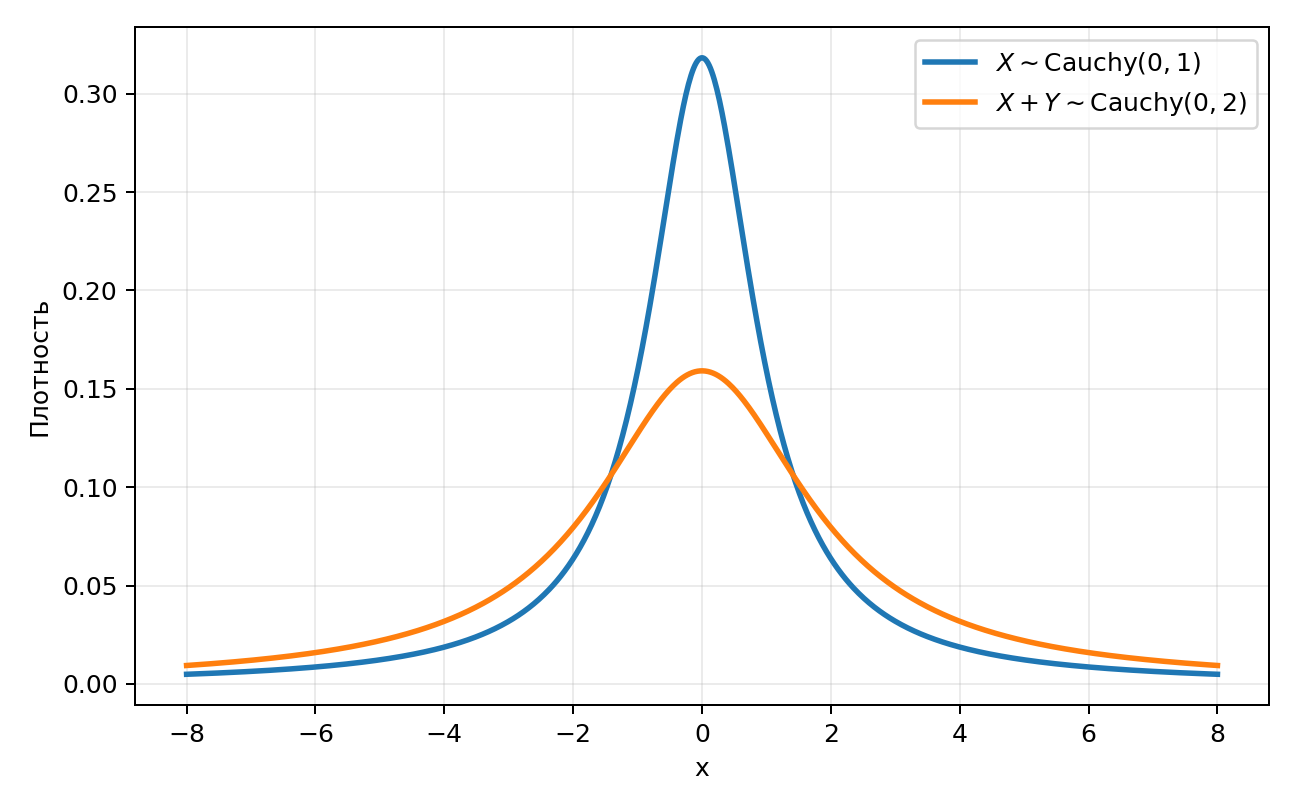
\includegraphics[keepaspectratio]{chapters/../assets/figures/cauchy_sum.png}}

}

\caption{Стандартное распределение Коши и распределение суммы двух
независимых стандартных величин Коши.}

\end{figure}%

У суммы максимум ниже, а распределение шире: параметр \(\gamma\)
увеличился с \(1\) до \(2\).

\end{bookfigurepanel}

\subsection{Алгоритм вычисления распределения суммы через
Фурье}\label{ux430ux43bux433ux43eux440ux438ux442ux43c-ux432ux44bux447ux438ux441ux43bux435ux43dux438ux44f-ux440ux430ux441ux43fux440ux435ux434ux435ux43bux435ux43dux438ux44f-ux441ux443ux43cux43cux44b-ux447ux435ux440ux435ux437-ux444ux443ux440ux44cux435}

Пусть независимые величины \(X\) и \(Y\) имеют плотности \(f_X(x)\) и
\(f_Y(y)\), а \[S=X+Y.\] Тогда вычисление можно организовать в три шага:

\begin{enumerate}
\def\labelenumi{\arabic{enumi}.}
\item
  Перейти от плотностей к характеристическим функциям: \[\varphi_X(t)
  =
  \int_{-\infty}^{+\infty}e^{itx}f_X(x)\,dx,
  \qquad
  \varphi_Y(t)
  =
  \int_{-\infty}^{+\infty}e^{ity}f_Y(y)\,dy.\]
\item
  Для независимой суммы перемножить характеристические функции:
  \[\boxed{
  \varphi_S(t)=\varphi_X(t)\varphi_Y(t).
  }\]
\item
  Вернуться к плотности обратным преобразованием Фурье: \[\boxed{
  f_S(s)
  =
  \frac{1}{2\pi}
  \int_{-\infty}^{+\infty}
  e^{-its}\varphi_S(t)\,dt.
  }\]
\end{enumerate}

\section{Свойства характеристической
функции}\label{ux441ux432ux43eux439ux441ux442ux432ux430-ux445ux430ux440ux430ux43aux442ux435ux440ux438ux441ux442ux438ux447ux435ux441ux43aux43eux439-ux444ux443ux43dux43aux446ux438ux438}

\subsection{Дискретный
случай}\label{ux434ux438ux441ux43aux440ux435ux442ux43dux44bux439-ux441ux43bux443ux447ux430ux439}

Если случайная величина \(X\) принимает дискретные значения \(x_k\) с
вероятностями \(p_k\), \[P(X=x_k)=p_k,
\qquad
\sum_k p_k=1,\] то интеграл в определении характеристической функции
заменяется суммой: \[\boxed{
\varphi_X(t)
=
\sum_k p_k e^{itx_k}.
}\] То есть характеристическая функция не вводит новую вероятностную
конструкцию: она лишь записывает уже известное распределение в форме,
удобной для работы с суммами.

\subsection{Почему характеристическая функция всегда
существует}\label{ux43fux43eux447ux435ux43cux443-ux445ux430ux440ux430ux43aux442ux435ux440ux438ux441ux442ux438ux447ux435ux441ux43aux430ux44f-ux444ux443ux43dux43aux446ux438ux44f-ux432ux441ux435ux433ux434ux430-ux441ux443ux449ux435ux441ux442ux432ux443ux435ux442}

Модуль комплексной экспоненты равен единице: \[\left|e^{itX}\right|=1.\]
Следовательно,
\[\left|\varphi_X(t)\right|=\left|\mathbb{E}\!\left[e^{itX}\right]\right|\leq
\mathbb{E}\!\left[\left|e^{itX}\right|\right]=1.\] Отсюда следует важное
свойство: \[\boxed{
|\varphi_X(t)|\leq 1.
}\]

\begin{booknote}

Характеристическая функция существует для любого распределения, в том
числе для распределений, у которых могут не существовать среднее
значение или дисперсия.

\end{booknote}

\subsection{Базовые
свойства}\label{ux431ux430ux437ux43eux432ux44bux435-ux441ux432ux43eux439ux441ux442ux432ux430}

Для любой случайной величины \(X\) выполняются соотношения: \[\boxed{
\varphi_X(0)=1,
\qquad
|\varphi_X(t)|\leq1,
\qquad
\varphi_X(-t)=\varphi_X^*(t).
}\] Первое равенство непосредственно следует из нормировки:
\[\varphi_X(0)
=
\mathbb{E}[e^0]
=
\mathbb{E}[1]
=1.\] Комплексное сопряжение экспоненты меняет знак перед \(t\), поэтому
\[\varphi_X(-t)=\varphi_X^*(t).\] Если распределение симметрично
относительно нуля, характеристическая функция вещественна и чётна. Кроме
того, характеристическая функция однозначно задаёт распределение.

\subsection{Сдвиг и
масштаб}\label{ux441ux434ux432ux438ux433-ux438-ux43cux430ux441ux448ux442ux430ux431}

Пусть новая случайная величина связана с \(X\) линейным преобразованием:
\[Y=aX+b.\] Тогда \[\varphi_Y(t)
=
\mathbb{E}\!\left[e^{it(aX+b)}\right] =
e^{itb}\,
\mathbb{E}\!\left[e^{i(at)X}\right].\] Следовательно, \[\boxed{
\varphi_{aX+b}(t)
=
e^{itb}\varphi_X(at).
}\] Если характеристическая функция исходной величины известна, то для
сдвинутой и масштабированной величины её можно получить сразу, без
нового интегрирования.

\section{Суммы многих независимых
величин}\label{ux441ux443ux43cux43cux44b-ux43cux43dux43eux433ux438ux445-ux43dux435ux437ux430ux432ux438ux441ux438ux43cux44bux445-ux432ux435ux43bux438ux447ux438ux43d}

В примере с распределением Коши мы доказали, что для двух независимых
случайных величин справедливо: \[\varphi_{X+Y}(t)
=
\varphi_X(t)\varphi_Y(t).\] Последовательно применяя это равенство к
сумме: \[S_n=X_1+X_2+\cdots+X_n,\] получаем: \[\boxed{
\varphi_{S_n}(t)
=
\prod_{k=1}^{n}\varphi_{X_k}(t).
}\] Если все \(X_k\) имеют одно и то же распределение, то их
характеристические функции совпадают и формула упрощается: \[\boxed{
\varphi_{S_n}(t)
=
\left[\varphi_X(t)\right]^n.
}\] Это свойство позволяет практически без интегрирования исследовать
целые семейства сумм.

\section{Примеры характеристических
функций}\label{ux43fux440ux438ux43cux435ux440ux44b-ux445ux430ux440ux430ux43aux442ux435ux440ux438ux441ux442ux438ux447ux435ux441ux43aux438ux445-ux444ux443ux43dux43aux446ux438ux439}

\subsection{Распределение
Бернулли}\label{ux440ux430ux441ux43fux440ux435ux434ux435ux43bux435ux43dux438ux435-ux431ux435ux440ux43dux443ux43bux43bux438}

Для распределения Бернулли случайная величина принимает только два
значения: \[X=0
\quad\text{или}\quad
X=1.\] Вероятности можно записать как: \[P(X=x)=p^x(1-p)^{1-x},
\qquad
x=0,1.\] В частности, \[P(X=0)=1-p,
\qquad
P(X=1)=p.\] По формуле для дискретного случая характеристическая функция
равна: \[\boxed{
\varphi_X(t)=(1-p)e^{it\cdot0}
+pe^{it\cdot1}=(1-p)+pe^{it}.}\]

Теперь возьмём сумму \(n\) независимых одинаково распределённых величин
Бернулли: \[S_n=X_1+\cdots+X_n.\] Её характеристическая функция:
\[\varphi_{S_n}(t)
=
\left[(1-p)+pe^{it}\right]^n.\] Раскроем скобки по биному Ньютона:
\[\left[(1-p)+pe^{it}\right]^n
=
\sum_{k=0}^{n}
\binom{n}{k}
(1-p)^{n-k}p^k e^{itk}.\] С другой стороны, для дискретной случайной
величины характеристическая функция имеет вид: \[\varphi_{S_n}(t)
=
\sum_{k=0}^{n}P(S_n=k)e^{itk}.\] Сравнивая коэффициенты при \(e^{itk}\),
получаем \[\boxed{
P(S_n=k)
=
\binom{n}{k}p^k(1-p)^{n-k}.
}\] Это биномиальное распределение: \[\boxed{
S_n\sim\mathrm{Bin}(n,p).
}\] Таким образом, сумма независимых величин Бернулли естественным
образом приводит к биномиальному распределению.

\subsection{Распределение
Пуассона}\label{ux440ux430ux441ux43fux440ux435ux434ux435ux43bux435ux43dux438ux435-ux43fux443ux430ux441ux441ux43eux43dux430}

Пусть \[N\sim\mathrm{Pois}(\lambda),\] то есть \[P(N=k)
=
e^{-\lambda}\frac{\lambda^k}{k!},
\qquad
k=0,1,2,\ldots\] Характеристическая функция равна:
\[\varphi_N(t)=\sum_{k=0}^{\infty}e^{itk}e^{-\lambda}\frac{\lambda^k}{k!}=e^{-\lambda}\sum_{k=0}^{\infty}
\frac{(\lambda e^{it})^k}{k!}.\] Сумма является разложением экспоненты в
ряд Тейлора: \[\sum_{k=0}^{\infty}
\frac{(\lambda e^{it})^k}{k!}
=
e^{\lambda e^{it}}.\] Поэтому \[\boxed{\varphi_N(t)=
e^{-\lambda}e^{\lambda e^{it}} =
e^{\lambda\left(e^{it}-1\right)}}.\]

\subsubsection{Сумма пуассоновских
величин}\label{ux441ux443ux43cux43cux430-ux43fux443ux430ux441ux441ux43eux43dux43eux432ux441ux43aux438ux445-ux432ux435ux43bux438ux447ux438ux43d}

Пусть независимые случайные величины имеют распределения
\[N_k\sim\mathrm{Pois}(\lambda_k),\] рассмотрим их сумму:
\[S_n=\sum_{k=1}^{n}N_k.\] Характеристическая функция суммы равна
произведению: \[\varphi_{S_n}(t)=
\prod_{k=1}^{n}\varphi_{N_k}(t)=\prod_{k=1}^{n}\exp\!\left[\lambda_k(e^{it}-1)\right]=
\exp\!\left[\left(\sum_{k=1}^{n}\lambda_k\right)(e^{it}-1)\right].\]
Обозначим \[\lambda=\sum_{k=1}^{n}\lambda_k.\] Тогда \[\varphi_{S_n}(t)
=
\exp\!\left[\lambda(e^{it}-1)\right],\] то есть снова получена
характеристическая функция распределения Пуассона.

\begin{booknote}

Сумма независимых пуассоновских случайных величин снова распределена по
Пуассону, причём параметры складываются: \[\boxed{
\sum_{k=1}^{n}N_k
\sim
\mathrm{Pois}\!\left(\sum_{k=1}^{n}\lambda_k\right).
}\]

\end{booknote}

\subsection{Распределение
Гаусса}\label{ux440ux430ux441ux43fux440ux435ux434ux435ux43bux435ux43dux438ux435-ux433ux430ux443ux441ux441ux430}

Пусть \[X\sim\mathrm{N}(\mu,\sigma^2).\] Плотность распределения имеет
вид: \[f_X(x)
=
\frac{1}{\sqrt{2\pi\sigma^2}}
\exp\!\left[-\frac{(x-\mu)^2}{2\sigma^2}\right].\] Тогда нетрудно
показать, что её характеристическая функция равна: \[\boxed{
\varphi_X(t)
=
\exp\!\left(
i\mu t-\frac{\sigma^2t^2}{2}
\right).
}\]

\begin{bookderivation}

\subsubsection{Вывод характеристической функции
Гаусса}\label{ux432ux44bux432ux43eux434-ux445ux430ux440ux430ux43aux442ux435ux440ux438ux441ux442ux438ux447ux435ux441ux43aux43eux439-ux444ux443ux43dux43aux446ux438ux438-ux433ux430ux443ux441ux441ux430}

Согласно определению: \[\varphi_X(t)
=
\int_{-\infty}^{+\infty}
e^{itx}
\frac{1}{\sqrt{2\pi\sigma^2}}
\exp\!\left[-\frac{(x-\mu)^2}{2\sigma^2}\right]dx.\] Представим \(x\)
как \((x-\mu)+\mu\) и вынесем множитель, не зависящий от переменной
интегрирования: \[\begin{aligned}
\varphi_X(t)
&=
e^{i\mu t}
\int_{-\infty}^{+\infty}
\frac{1}{\sqrt{2\pi\sigma^2}}
\exp\!\left[
-\frac{(x-\mu)^2}{2\sigma^2}
+it(x-\mu)
\right]dx.
\end{aligned}\] В показателе экспоненты дополним выражение до полного
квадрата: \[-\frac{(x-\mu)^2}{2\sigma^2}
+it(x-\mu)
=
-\frac{(x-\mu-i\sigma^2t)^2}{2\sigma^2}
-\frac{\sigma^2t^2}{2}.\] Тогда \[\begin{aligned}
\varphi_X(t)
&=
e^{i\mu t-\sigma^2t^2/2}
\int_{-\infty}^{+\infty}
\frac{1}{\sqrt{2\pi\sigma^2}}
\exp\!\left[
-\frac{(x-\mu-i\sigma^2t)^2}{2\sigma^2}
\right]dx.
\end{aligned}\] Оставшийся интеграл после соответствующего сдвига имеет
нормировку гауссова интеграла и даёт единицу: \[\boxed{
\varphi_X(t)
=
e^{i\mu t-\sigma^2t^2/2}.
} \quad \blacksquare\]

\end{bookderivation}

\subsubsection{Сумма гауссовых
величин}\label{ux441ux443ux43cux43cux430-ux433ux430ux443ux441ux441ux43eux432ux44bux445-ux432ux435ux43bux438ux447ux438ux43d}

Пусть независимые величины распределены как
\[X_k\sim\mathrm{N}(\mu_k,\sigma_k^2).\] Тогда для их суммы
\[S_n=\sum_{k=1}^{n}X_k\] получаем характеристическую функцию:
\[\begin{aligned}
\varphi_{S_n}(t)
&=
\prod_{k=1}^{n}
\exp\!\left(
i\mu_k t-\frac{\sigma_k^2t^2}{2}
\right) \\
&=
\exp\!\left[
i t\sum_{k=1}^{n}\mu_k
-
\frac{t^2}{2}\sum_{k=1}^{n}\sigma_k^2
\right].
\end{aligned}\] Таким образом, сумма независимых гауссовых величин
распределена по гауссу: \[\boxed{
S_n
\sim
\mathrm{N}\!\left(
\sum_{k=1}^{n}\mu_k,
\sum_{k=1}^{n}\sigma_k^2
\right).
}\] Видно, что \textbf{средние значения, как и дисперсии, просто
складываются}.

\subsection{Распределение
Коши}\label{ux440ux430ux441ux43fux440ux435ux434ux435ux43bux435ux43dux438ux435-ux43aux43eux448ux438}

Пусть независимые величины распределены как
\[X_k\sim\mathrm{Cauchy}(0,1).\] Для каждой из них
\[\varphi_{X_k}(t)=e^{-|t|}.\] Поэтому характеристическая функция суммы
\[S_n=X_1+\cdots+X_n\] равна \[\varphi_{S_n}(t)
=
\left(e^{-|t|}\right)^n
=
e^{-n|t|}.\] Следовательно, \[S_n\sim\mathrm{Cauchy}(0,n).\] Теперь
разделим сумму на \(n\). Используя правило масштабирования
характеристической функции, получаем \[\boxed{
\frac{S_n}{n}
\sim
\mathrm{Cauchy}(0,1).
}\] То есть среднее арифметическое таких величин имеет то же
распределение Коши, что и каждое отдельное слагаемое. Обратите внимание,
данное выражением понадобится для последующего обсуждения условий
применимости центральной предельной теоремы.

\section{Моменты из характеристической
функции}\label{ux43cux43eux43cux435ux43dux442ux44b-ux438ux437-ux445ux430ux440ux430ux43aux442ux435ux440ux438ux441ux442ux438ux447ux435ux441ux43aux43eux439-ux444ux443ux43dux43aux446ux438ux438}

Характеристическая функция полезна не только для сумм случайных величин.
В ней непосредственно содержится информация о моментах распределения.
Начнём с определения: \[\varphi_X(t)
=
\mathbb{E}\!\left[e^{itX}\right].\] Разложим экспоненту в ряд Тейлора:
\[e^{itX}
=
\sum_{n=0}^{\infty}
\frac{(itX)^n}{n!}.\] Тогда формально \[\varphi_X(t)=
\mathbb{E}\!\left[\sum_{n=0}^{\infty}\frac{(itX)^n}{n!}\right]=\sum_{n=0}^{\infty}\frac{(it)^n}{n!}\mathbb{E}[X^n].\]
Таким образом, коэффициенты разложения характеристической функции
связаны с моментами \(\mathbb{E}[X^n]\).

Если взять \(n\)-ю производную по \(t\) и затем положить \(t=0\), все
члены, кроме соответствующего \(n\)-му моменту, исчезнут. Получим
\[\boxed{
\varphi_X^{(n)}(0)
=
i^n\mathbb{E}[X^n].
}\] Или \[\boxed{
\mathbb{E}[X^n]
=
\frac{1}{i^n}\varphi_X^{(n)}(0).
}\] В частности, \[\mathbb{E}[X]
=
\frac{\varphi_X'(0)}{i},
\qquad
\mathbb{E}[X^2]
=
-\varphi_X''(0).\]

\subsection{Почему у распределения Коши возникают проблемы с
моментами}\label{ux43fux43eux447ux435ux43cux443-ux443-ux440ux430ux441ux43fux440ux435ux434ux435ux43bux435ux43dux438ux44f-ux43aux43eux448ux438-ux432ux43eux437ux43dux438ux43aux430ux44eux442-ux43fux440ux43eux431ux43bux435ux43cux44b-ux441-ux43cux43eux43cux435ux43dux442ux430ux43cux438}

Характеристическая функция существует всегда, но её производные
требуемого порядка могут не существовать. Например, для стандартного
распределения Коши: \[\varphi_X(t)=e^{-|t|}.\] Из-за модуля эта функция
не дифференцируема в точке \(t=0\). Обратите внимание, распределение
Коши имеет вполне определённую плотность вероятности и по ней можно
генерировать случайные величины, однако обычные моменты -- в том числе
среднее -- у него не существуют.

\section{Кумулянты}\label{ux43aux443ux43cux443ux43bux44fux43dux442ux44b}

\begin{booknote}

Следующий полезный объект строится из логарифма характеристической
функции. Определим \[\boxed{
K_X(t)=\ln\varphi_X(t).
}\] Это \textbf{производящая функция кумулянтов}. Разложим её около
нуля: \[\boxed{
K_X(t)
=
\sum_{n=1}^{\infty}
\kappa_n\frac{(it)^n}{n!}.
}\] Коэффициенты \(\kappa_n\) называются \textbf{кумулянтами}. Как и
моменты, их можно извлечь при помощи производных: \[\boxed{
\kappa_n
=
\frac{1}{i^n}
\left.
\frac{d^n}{dt^n}
\ln\varphi_X(t)
\right|_{t=0}.
}\]

\end{booknote}

\begin{bookderivation}

\subsection{Вывод первых двух
кумулянтов}\label{ux432ux44bux432ux43eux434-ux43fux435ux440ux432ux44bux445-ux434ux432ux443ux445-ux43aux443ux43cux443ux43bux44fux43dux442ux43eux432}

Поскольку \[K_X(t)=\ln\varphi_X(t),\] первая производная равна:
\[K_X'(t)
=
\frac{\varphi_X'(t)}{\varphi_X(t)}.\] При \(t=0\) имеем
\(\varphi_X(0)=1\) и \[\varphi_X'(0)=i\mathbb{E}[X].\] Поэтому \[K_X'(0)
=
i\mathbb{E}[X].\] С учётом определения кумулянта \[\boxed{
\kappa_1
=
\mathbb{E}[X]
=
\mu.
}\] Для второй производной: \[K_X''(t)
=
\frac{\varphi_X''(t)}{\varphi_X(t)}
-
\left(
\frac{\varphi_X'(t)}{\varphi_X(t)}
\right)^2.\] В нуле: \[\varphi_X''(0)=-\mathbb{E}[X^2],
\qquad
\varphi_X'(0)=i\mathbb{E}[X],\] поэтому \[\begin{aligned}
K_X''(0)
&=
-\mathbb{E}[X^2]
+\mathbb{E}[X]^2=
-\operatorname{Var}(X).
\end{aligned}\] Так как \(i^2=-1\), \[\boxed{
\kappa_2
=
\operatorname{Var}(X)
=
\sigma^2.
} \quad \blacksquare\]

\end{bookderivation}

Первые два кумулянта, таким образом, имеют непосредственный
статистический смысл: это среднее значение и дисперсия.

\begin{bookderivation}

\subsection{Вывод следующих
кумулянтов}\label{ux432ux44bux432ux43eux434-ux441ux43bux435ux434ux443ux44eux449ux438ux445-ux43aux443ux43cux443ux43bux44fux43dux442ux43eux432}

Для дальнейшего разложения удобно перейти к центрированной случайной
величине \[Y=X-\mu\] и обозначить её центральные моменты как:
\[m_r=\mathbb{E}[Y^r].\] В частности, \[m_2=\sigma^2.\] Из свойства
сдвига следует: \[K_Y(t)=K_X(t)-i\mu t,\] то есть центрирование изменяет
только первый кумулянт. Характеристическая функция центрированной
величины около нуля имеет разложение: \[\varphi_Y(t)
=
1-
\frac{m_2t^2}{2}
-i\frac{m_3t^3}{6}
+
\frac{m_4t^4}{24}
+O(t^5).\] Используя разложение \[\ln(1+u)
=
u-\frac{u^2}{2}+\cdots,\] получаем: \[K_Y(t)
=
-\frac{m_2t^2}{2}
-i\frac{m_3t^3}{6}
+
\frac{(m_4-3m_2^2)t^4}{24}
+O(t^5).\] Сравнивая коэффициенты при степенях \(it\), находим первые
четыре кумулянта: \[\boxed{
\begin{aligned}
\kappa_1&=\mu,\\
\kappa_2&=\sigma^2,\\
\kappa_3&=\mathbb{E}[(X-\mu)^3],\\
\kappa_4&=\mathbb{E}[(X-\mu)^4]-3\sigma^4.
\end{aligned}
} \quad \blacksquare\]

\end{bookderivation}

\subsection{Почему кумулянты удобны для
сумм}\label{ux43fux43eux447ux435ux43cux443-ux43aux443ux43cux443ux43bux44fux43dux442ux44b-ux443ux434ux43eux431ux43dux44b-ux434ux43bux44f-ux441ux443ux43cux43c}

Пусть \(X\) и \(Y\) независимы. Тогда \[\varphi_{X+Y}(t)
=
\varphi_X(t)\varphi_Y(t).\] Возьмём логарифм: \[\begin{aligned}
K_{X+Y}(t)
&=
\ln\varphi_{X+Y}(t) \\
&=
\ln\varphi_X(t)
+
\ln\varphi_Y(t) \\
&=
K_X(t)+K_Y(t).
\end{aligned}\] Следовательно, коэффициенты разложения также
складываются: \[\boxed{
\kappa_n(X+Y)
=
\kappa_n(X)+\kappa_n(Y).
}\] Это существенное отличие от обычных моментов: при раскрытии моментов
суммы появляются смешанные члены, а кумулянты независимых величин просто
складываются.

Для масштабирования случайной величины выполняется: \[\boxed{
\kappa_n(aX)
=
a^n\kappa_n(X).
}\] Оба свойства особенно удобны при исследовании нормированных сумм.

\section{Мост к центральной предельной
теореме}\label{ux43cux43eux441ux442-ux43a-ux446ux435ux43dux442ux440ux430ux43bux44cux43dux43eux439-ux43fux440ux435ux434ux435ux43bux44cux43dux43eux439-ux442ux435ux43eux440ux435ux43cux435}

В этой главе мы не будем формулировать центральную предельную теорему в
полном виде. Вместо этого характеристические функции используются, чтобы
показать, почему гауссовское распределение естественно возникает для
нормированных сумм большого числа независимых одинаково распределённых
величин.

Пусть \(X_1,\ldots,X_n\) -- независимые и одинаково распределённые
случайные величины, для которых: \[\mathbb{E}[X_k]=\mu,
\qquad
\operatorname{Var}(X_k)=\sigma^2<\infty.\] Условие конечности дисперсии
здесь принципиально важно. Рассмотрим нормированную сумму: \[\boxed{
Z_n
=
\frac{1}{\sigma\sqrt n}
\sum_{k=1}^{n}(X_k-\mu).
}\]

\subsection{Центрирование и
нормировка}\label{ux446ux435ux43dux442ux440ux438ux440ux43eux432ux430ux43dux438ux435-ux438-ux43dux43eux440ux43cux438ux440ux43eux432ux43aux430}

Введём: \[Y_k
=
\frac{X_k-\mu}{\sigma}.\] Тогда \[\mathbb{E}[Y_k]=0,
\qquad
\operatorname{Var}(Y_k)=1,\] и \[Z_n
=
\frac{Y_1+Y_2+\cdots+Y_n}{\sqrt n}.\] Используя правило масштабирования
и произведение характеристических функций независимых величин, получаем:
\[\boxed{
\varphi_{Z_n}(t)
=
\left[
\varphi_Y\!\left(\frac{t}{\sqrt n}\right)
\right]^n.
}\]

\subsection{Разложение характеристической функции около
нуля}\label{ux440ux430ux437ux43bux43eux436ux435ux43dux438ux435-ux445ux430ux440ux430ux43aux442ux435ux440ux438ux441ux442ux438ux447ux435ux441ux43aux43eux439-ux444ux443ux43dux43aux446ux438ux438-ux43eux43aux43eux43bux43e-ux43dux443ux43bux44f}

Не будем предполагать конкретного вида распределения \(Y_k\), а
воспользуемся только тем, что \[\mathbb{E}[Y_k]=0,
\qquad
\operatorname{Var}(Y_k)=1.\] При малом аргументе \(u\) разложение
характеристической функции начинается как: \[\varphi_Y(u)
=
1-\frac{u^2}{2}+o(u^2).\] Подставим \[u=\frac{t}{\sqrt n}.\] Тогда
\[\varphi_Y\!\left(\frac{t}{\sqrt n}\right)
=
1-
\frac{t^2}{2n}
+o\!\left(\frac{1}{n}\right).\] Следовательно, \[\boxed{
\varphi_{Z_n}(t)
=
\left[
1-
\frac{t^2}{2n}
+o\!\left(\frac{1}{n}\right)
\right]^n.
}\]

\subsection{Предел при большом числе
слагаемых}\label{ux43fux440ux435ux434ux435ux43b-ux43fux440ux438-ux431ux43eux43bux44cux448ux43eux43c-ux447ux438ux441ux43bux435-ux441ux43bux430ux433ux430ux435ux43cux44bux445}

Используем известный предел: \[\lim_{n\to\infty}
\left(1+\frac{x}{n}\right)^n
=e^x.\] В нашем случае: \[x=-\frac{t^2}{2}.\] В итоге, \[\boxed{
\lim_{n\to\infty}
\varphi_{Z_n}(t)
=
e^{-t^2/2}.
}\] Это характеристическая функция стандартного распределения Гаусса
\(\mathrm{N}(0,1)\). Таким \textbf{образом, сумма бесконечно большого
числа независимых и одинаково распределенных величин с конечной
дисперсией стремится к гауссову распределению.}

Обратите внимание, приведённое рассуждение рассматривает важный случай
независимых \textbf{одинаково распределённых} величин и служит мостом к
более подробному обсуждению центральной предельной теоремы в следующей
главе. Главный результат этого рассуждения состоит в том, что исходный
вид распределения отдельных \(X_k\) не фиксировался. Использовались лишь
их среднее значение, дисперсия, независимость и одинаковость
распределения.

\subsection{Почему в пределе появляется именно
Гаусс}\label{ux43fux43eux447ux435ux43cux443-ux432-ux43fux440ux435ux434ux435ux43bux435-ux43fux43eux44fux432ux43bux44fux435ux442ux441ux44f-ux438ux43cux435ux43dux43dux43e-ux433ux430ux443ux441ux441}

После центрирования и нормировки более высокие детали исходного
распределения подавляются при увеличении \(n\). В пределе остаётся
квадратичный член: \[\ln\varphi(t)
\simeq
-\frac{t^2}{2},\] который соответствует характеристической функции
Гаусса. Тот же результат особенно наглядно виден через кумулянты. Для
\[Z_n
=
\frac{1}{\sqrt n}
\sum_{k=1}^{n}Y_k\] кумулянт порядка \(r\) масштабируется как:
\[\kappa_r(Z_n)=
\frac{1}{n^{r/2}}
\sum_{k=1}^{n}\kappa_r(Y_k) =
n^{1-r/2}\kappa_r(Y).\] Таким образом, \[\boxed{
\kappa_r(Z_n)
\propto
n^{1-r/2}.
}\] При \(r=2\) дисперсия остаётся равной единице. Для всех порядков
\(r>2\) соответствующий множитель стремится к нулю при \(n\to\infty\):
\[\kappa_3(Z_n)\propto\frac{1}{\sqrt n},
\qquad
\kappa_4(Z_n)\propto\frac{1}{n}, \quad \text{и т.д.}\]

\section{Интерактив: приближение к распределению Гаусса в пространстве
Фурье}\label{ux438ux43dux442ux435ux440ux430ux43aux442ux438ux432-ux43fux440ux438ux431ux43bux438ux436ux435ux43dux438ux435-ux43a-ux440ux430ux441ux43fux440ux435ux434ux435ux43bux435ux43dux438ux44e-ux433ux430ux443ux441ux441ux430-ux432-ux43fux440ux43eux441ux442ux440ux430ux43dux441ux442ux432ux435-ux444ux443ux440ux44cux435}

Возьмем независимые случайные величины: \[X_k\sim U(-\sqrt3,\sqrt3),\]
для которых выполняется: \[\mathbb{E}[X_k]=0,
\qquad
\operatorname{Var}(X_k)=1.\] На графике по горизонтальной оси
откладывается аргумент \(t\), а по вертикальной -- вещественная часть
характеристической функции. Сравниваются характеристическая функция
нормированной суммы и предельная функция \[e^{-t^2/2}.\]

При \(n=1\) между ними ещё хорошо видны отличия и колебания.

\begin{bookfigurepanel}

\begin{center}

\pandocbounded{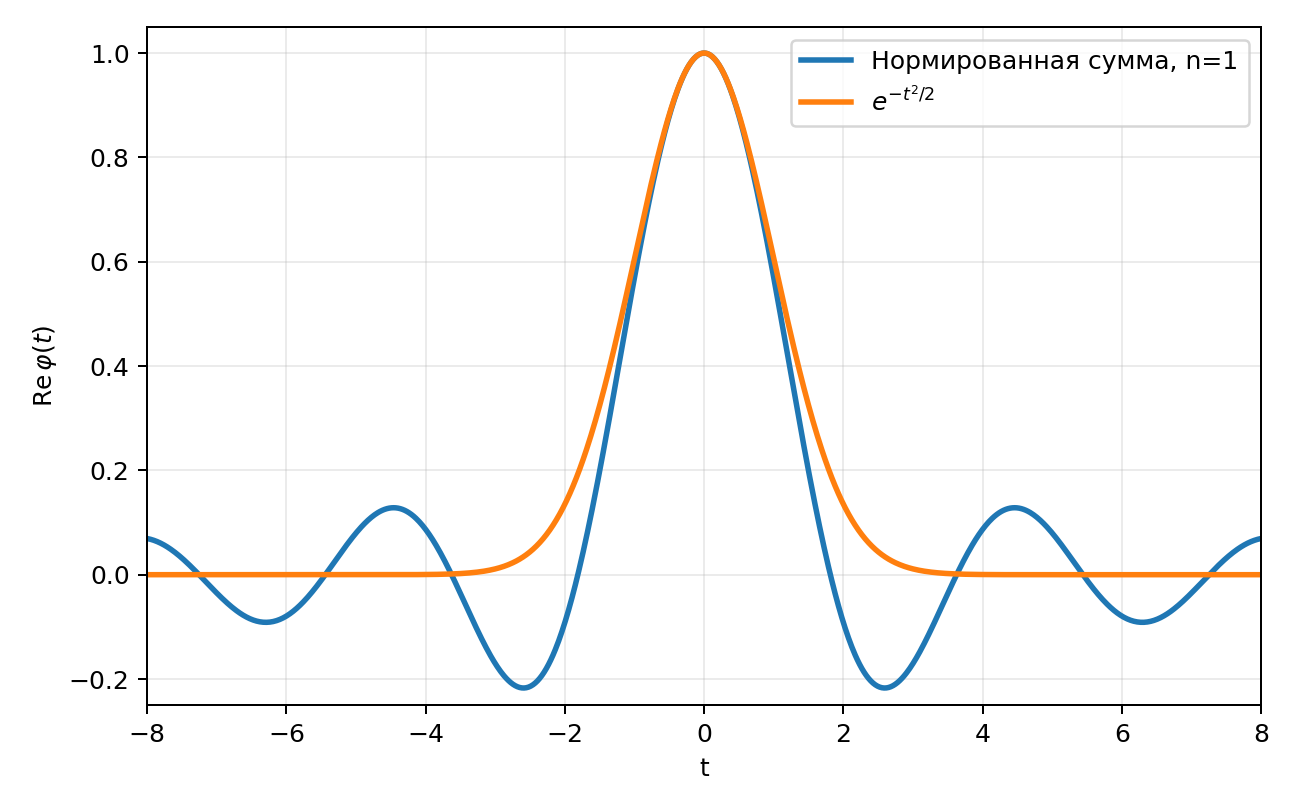
\includegraphics[keepaspectratio,alt={При одном слагаемом характеристическая функция равномерного распределения ещё заметно отличается от Гуасса. Статическая версия интерактивного графика из лекции.}]{chapters/../assets/figures/clt_fourier_n1.png}}

\end{center}

\BookInlineFigureCaption{При одном слагаемом характеристическая функция равномерного
распределения ещё заметно отличается от Гуасса. Статическая версия
интерактивного графика из лекции.}

\end{bookfigurepanel}

По мере увеличения числа слагаемых колебания становятся всё меньше. В
лекции отмечается, что примерно при \(n=10-11\) две кривые уже трудно
различить на глаз.

\begin{bookfigurepanel}

\begin{center}

\pandocbounded{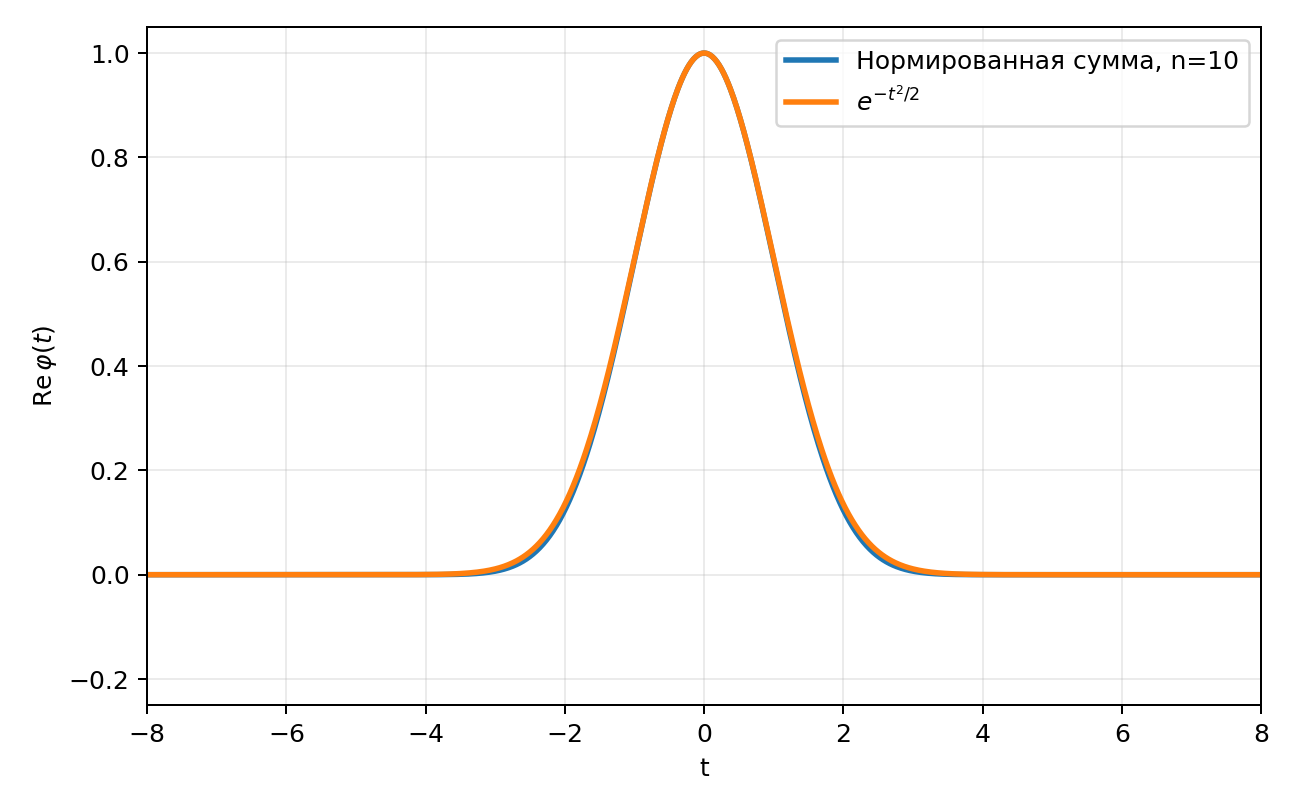
\includegraphics[keepaspectratio,alt={При десяти слагаемых характеристическая функция нормированной суммы уже близка к e\^{}\{-t\^{}2/2\}. Статическая версия интерактивного графика из лекции.}]{chapters/../assets/figures/clt_fourier_n10.png}}

\end{center}

\BookInlineFigureCaption{При десяти слагаемых характеристическая функция нормированной суммы уже
близка к \(e^{-t^2/2}\). Статическая версия интерактивного графика из
лекции.}

\end{bookfigurepanel}

\begin{bookchaptersummary}[Итоги главы]

\begin{itemize}
\tightlist
\item
  Характеристическая функция -- это преобразование Фурье распределения:
  \[\varphi_X(t)=\mathbb{E}[e^{itX}].\]
\item
  Для суммы независимых случайных величин характеристические функции
  перемножаются, поэтому свёртки удобно вычислять в пространстве Фурье.
\item
  Характеристическая функция существует для любого распределения, хотя
  её производные нужного порядка могут не существовать.
\item
  Моменты связаны с производными характеристической функции в точке
  \(t=0\).
\item
  Кумулянты задаются коэффициентами разложения \(\ln\varphi_X(t)\) и для
  независимых сумм просто складываются.
\item
  ЦПТ естественно возникает из квадратичного члена разложения
  \(\ln\varphi(t)\).
\item
  Для распределения Коши сумма остаётся распределением Коши;
  нормированная сумма \(S_n/n\) имеет то же распределение
  \(\mathrm{Cauchy}(0,1)\). Особую роль в этом играет условие конечной
  дисперсии.
\end{itemize}

\end{bookchaptersummary}

\section{Материалы
курса}\label{ux43cux430ux442ux435ux440ux438ux430ux43bux44b-ux43aux443ux440ux441ux430}

\begin{itemize}
\tightlist
\item
  \href{https://neutrinohit.github.io/statistical-analysis-course/ru/slides/02_characteristic_functions.html}{Слайды
  лекции}
\item
  \href{https://neutrinohit.github.io/statistical-analysis-course/ru/slides/exercises/02_characteristic_functions_exercises.html}{Задачи}
\end{itemize}

\chapter{Центральная предельная теорема и нормальное
распределение}\label{ux446ux435ux43dux442ux440ux430ux43bux44cux43dux430ux44f-ux43fux440ux435ux434ux435ux43bux44cux43dux430ux44f-ux442ux435ux43eux440ux435ux43cux430-ux438-ux43dux43eux440ux43cux430ux43bux44cux43dux43eux435-ux440ux430ux441ux43fux440ux435ux434ux435ux43bux435ux43dux438ux435}

\begin{bookchapteropening}[Главная мысль]

Центральная предельная теорема объясняет, почему при сложении большого
числа независимых случайных вкладов с конечными дисперсиями возникает
нормальное распределение. После центрирования и нормировки сумма
стремится к стандартному гауссу, а квантили этого распределения
позволяют количественно задавать вероятностные интервалы и проверять
совместимость измерений с учётом их неопределённостей.

\end{bookchapteropening}

\section{План
главы}\label{ux43fux43bux430ux43d-ux433ux43bux430ux432ux44b-2}

\begin{itemize}
\tightlist
\item
  Псевдослучайные числа и равномерный генератор
\item
  Суммы случайных величин
\item
  Среднее, дисперсия и ковариация суммы
\item
  Центральная предельная теорема
\item
  Гауссово распределение, стандартизация и квантили
\item
  Центральные интервалы в единицах \(\sigma\)
\item
  Проверка совместимости двух независимых измерений
\end{itemize}

\section{Псевдослучайные
числа}\label{ux43fux441ux435ux432ux434ux43eux441ux43bux443ux447ux430ux439ux43dux44bux435-ux447ux438ux441ux43bux430}

При работе с модельными данными часто требуется генерировать случайные
числа на компьютере. Такие числа называют \textbf{псевдослучайными}:
последовательность строится алгоритмом и в теории когда-нибудь начнёт
повторяться. Современные генераторы имеют настолько длинный период, что
в практических вычислениях эту последовательность можно рассматривать
как случайную.

\begin{booknote}

Для дальнейшей работы достаточно уметь получать равномерно
распределённую случайную величину:

\[X\sim U(-1,1).\]

Имея генератор равномерного распределения, можно строить генераторы для
других распределений. Детали самих алгоритмов генерации здесь не нужны:
важно уметь корректно пользоваться готовым генератором.

\end{booknote}

Одна из простых реализаций на Python выглядит так:

\begin{Shaded}
\begin{Highlighting}[]
\ImportTok{import}\NormalTok{ numpy }\ImportTok{as}\NormalTok{ np}

\NormalTok{rng }\OperatorTok{=}\NormalTok{ np.random.default\_rng(}\DecValTok{7}\NormalTok{)}
\NormalTok{x }\OperatorTok{=}\NormalTok{ rng.uniform(}\OperatorTok{{-}}\DecValTok{1}\NormalTok{, }\DecValTok{1}\NormalTok{, size}\OperatorTok{=}\DecValTok{20\_000}\NormalTok{)}
\end{Highlighting}
\end{Shaded}

Команда \texttt{default\_rng(7)} создаёт воспроизводимый генератор, а
\texttt{uniform(-1,\ 1,\ size=20\_000)} формирует массив из двадцати
тысяч значений в интервале от \(-1\) до \(1\).

\begin{bookfigurepanel}

\begin{center}

\pandocbounded{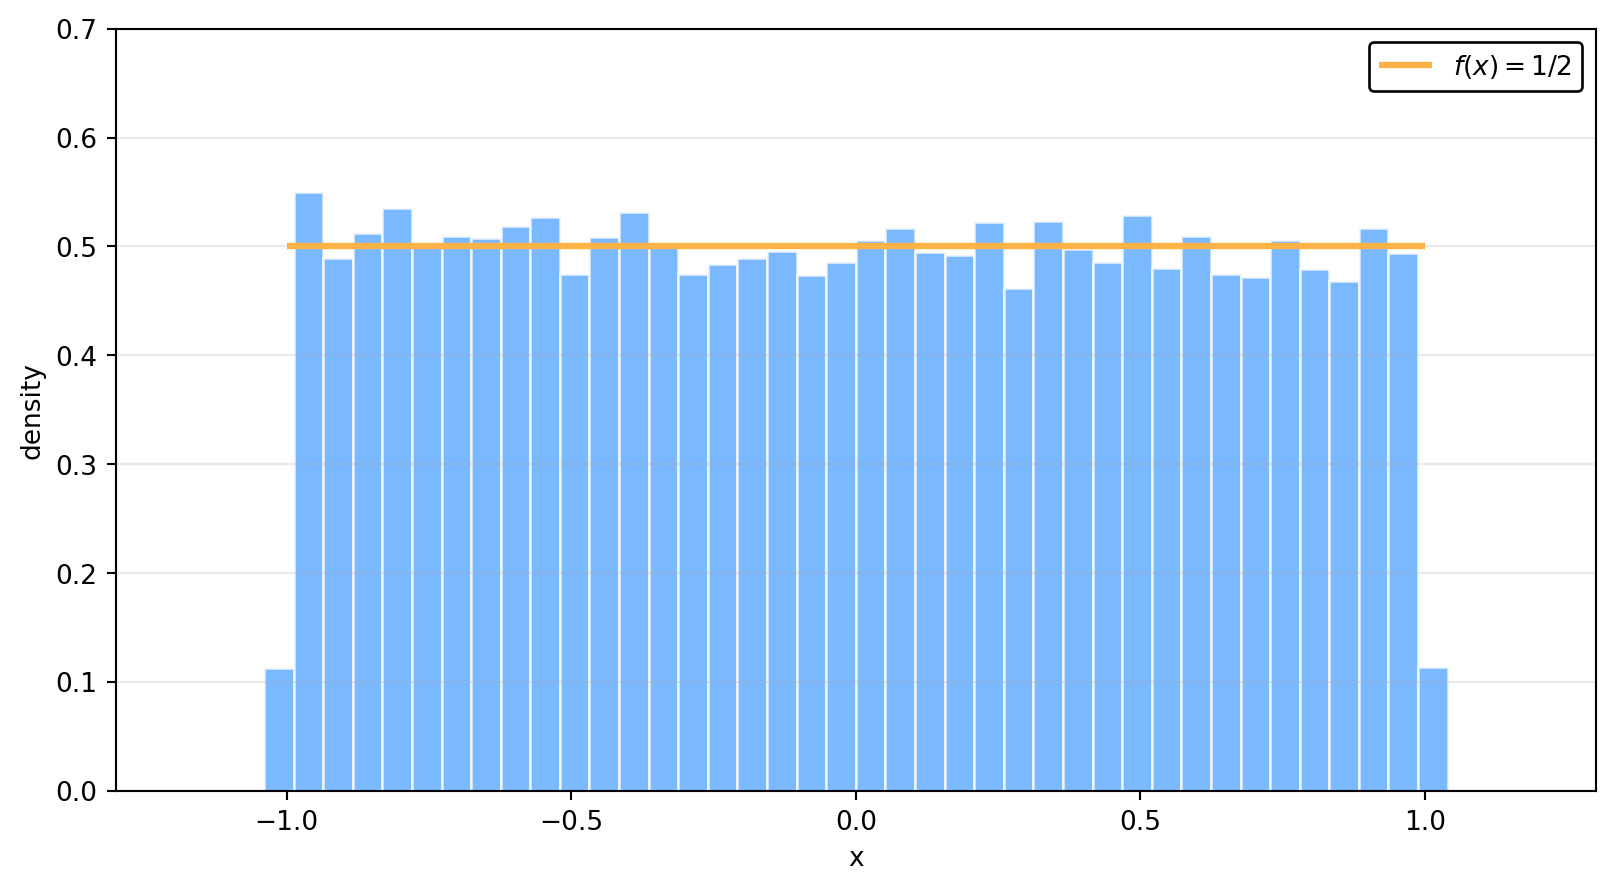
\includegraphics[keepaspectratio,alt={Выборка из равномерного распределения U(-1,1). Оранжевая линия показывает плотность f(x)=1/2.}]{chapters/../assets/figures/clt_uniform_sample.png}}

\end{center}

\BookInlineFigureCaption{Выборка из равномерного распределения \(U(-1,1)\). Оранжевая линия
показывает плотность \(f(x)=1/2\).}

Для равномерного распределения на интервале \([-1,1]\) плотность
постоянна и равна \(1/2\), так как площадь под плотностью должна быть
единичной.

\end{bookfigurepanel}

Глядя только на несколько отдельных чисел, невозможно увидеть форму
распределения. Гистограмма большой выборки показывает, что значения
действительно заполняют весь интервал примерно равномерно и флуктуируют
вокруг постоянной плотности.

\section{Сумма случайных
величин}\label{ux441ux443ux43cux43cux430-ux441ux43bux443ux447ux430ux439ux43dux44bux445-ux432ux435ux43bux438ux447ux438ux43d}

Пусть имеется набор независимых случайных величин:

\[X_1,X_2,\ldots,X_m,\] и построена их сумма:
\[\boxed{S_m=X_1+X_2+\cdots+X_m.}\] Вопрос: как меняется распределение
\(S_m\) при увеличении числа слагаемых (\(m\rightarrow \infty\))?

В качестве конкретного примера рассмотрим одинаково распределённые
независимые величины:

\[X_i\sim U(-1,1).\] Каждая из них принимает значения только между
\(-1\) и \(1\). Сама сумма при увеличении \(m\) уже может занимать всё
более широкий интервал, и заранее форма её распределения не очевидна.

\subsection{Среднее и дисперсия одного равномерного
вклада}\label{ux441ux440ux435ux434ux43dux435ux435-ux438-ux434ux438ux441ux43fux435ux440ux441ux438ux44f-ux43eux434ux43dux43eux433ux43e-ux440ux430ux432ux43dux43eux43cux435ux440ux43dux43eux433ux43e-ux432ux43aux43bux430ux434ux430}

Из симметрии распределения сразу видно, что \[\mathbb{E}[X_i]=0.\]
Дисперсию вычислим явно.

\begin{bookderivation}

\subsubsection{\texorpdfstring{Вывод \(\mathrm{Var}(X_i)\) для
\(X_i\sim U(-1,1)\)}{Вывод \textbackslash mathrm\{Var\}(X\_i) для X\_i\textbackslash sim U(-1,1)}}\label{ux432ux44bux432ux43eux434-mathrmvarx_i-ux434ux43bux44f-x_isim-u-11}

Плотность равномерного распределения на \([-1,1]\) равна

\[f(x)=\frac12.\]

Второй момент:

\[\mathbb{E}[X_i^2]
=\int_{-1}^{1}x^2\frac12\,dx=\frac12\left[\frac{x^3}{3}\right]_{-1}^{1}=\frac12\cdot\frac{2}{3}
=\frac13.\]

Согласно определению дисперсии:

\[\mathrm{Var}(X_i)
=\mathbb{E}[X_i^2]-\mathbb{E}[X_i]^2.\]

Так как \(\mathbb{E}[X_i]=0\), то в итоге получаем:

\[\boxed{\mathrm{Var}(X_i)=\frac13.}\quad\blacksquare\]

\end{bookderivation}

\subsection{Среднее
суммы}\label{ux441ux440ux435ux434ux43dux435ux435-ux441ux443ux43cux43cux44b}

Воспользуемся линейностью математического ожидания:

\[\mathbb{E}[S_m]=\mathbb{E}\!\left[\sum_{i=1}^{m}X_i\right]=\sum_{i=1}^{m}\mathbb{E}[X_i].\]
Для рассматриваемого примера каждое среднее равно нулю, следовательно,
\[\boxed{\mathbb{E}[S_m]=0.}\]

\subsection{Ковариация и дисперсия
суммы}\label{ux43aux43eux432ux430ux440ux438ux430ux446ux438ux44f-ux438-ux434ux438ux441ux43fux435ux440ux441ux438ux44f-ux441ux443ux43cux43cux44b}

При вычислении дисперсии суммы появляются не только квадраты отдельных
вкладов, но и произведения величин с разными индексами. Эти смешанные
члены естественно приводят к понятию ковариации.

\begin{booknote}

\textbf{Ковариация} двух случайных величин \(X\) и \(Y\) определяется
как:

\[\boxed{
\mathrm{cov}(X,Y)
=\mathbb{E}\!\left[(X-\mathbb{E}[X])(Y-\mathbb{E}[Y])\right]
=\mathbb{E}[XY]-\mathbb{E}[X]\mathbb{E}[Y].
}\]

Если \(X=Y\), получаем дисперсию:

\[\mathrm{cov}(X,X)=\mathrm{Var}(X).\]

\end{booknote}

\begin{bookderivation}

\subsubsection{Вывод дисперсии
суммы}\label{ux432ux44bux432ux43eux434-ux434ux438ux441ux43fux435ux440ux441ux438ux438-ux441ux443ux43cux43cux44b}

Соглсно определению:

\[\mathrm{Var}(S_m)
=\mathbb{E}\!\left[(S_m-\mathbb{E}[S_m])^2\right].\]

Подставим сумму:

\[\mathrm{Var}(S_m)
=
\mathbb{E}\!\left[
\left(
\sum_{i=1}^{m}(X_i-\mathbb{E}[X_i])
\right)^2
\right].\]

После раскрытия квадрата возникают два типа членов: с одинаковыми и с
различными индексами:

\[\begin{aligned}
\mathrm{Var}(S_m)
={}&
\sum_{i=1}^{m}
\mathbb{E}\!\left[(X_i-\mathbb{E}[X_i])^2\right]\\
&+2\sum_{i<j}
\mathbb{E}\!\left[(X_i-\mathbb{E}[X_i])(X_j-\mathbb{E}[X_j])\right].
\end{aligned}\]

Используя определения дисперсии и ковариации, получаем:

\[\boxed{
\mathrm{Var}(S_m)
=
\sum_{i=1}^{m}\mathrm{Var}(X_i)
+2\sum_{i<j}\mathrm{cov}(X_i,X_j).
}\]

Если величины независимы, их ковариации равны нулю:

\[\mathrm{Var}(S_m)
=
\sum_{i=1}^{m}\mathrm{Var}(X_i).\]

Для \(X_i\sim U(-1,1)\) каждая дисперсия равна \(1/3\), следовательно:

\[\boxed{\mathrm{Var}(S_m)=\frac{m}{3}.}\quad\blacksquare\]

\end{bookderivation}

Обратите внимание: независимость здесь является существенным условием.
Если между слагаемыми есть корреляции, смешанные члены не исчезают и
дисперсия суммы ведёт себя иначе.

\section{Центральная предельная
теорема}\label{ux446ux435ux43dux442ux440ux430ux43bux44cux43dux430ux44f-ux43fux440ux435ux434ux435ux43bux44cux43dux430ux44f-ux442ux435ux43eux440ux435ux43cux430}

Теперь можно сформулировать основное утверждение.

\begin{booknote}

\subsection{Центральная предельная
теорема}\label{ux446ux435ux43dux442ux440ux430ux43bux44cux43dux430ux44f-ux43fux440ux435ux434ux435ux43bux44cux43dux430ux44f-ux442ux435ux43eux440ux435ux43cux430-1}

Если \(X_1,\ldots,X_m\) независимы и имеют конечные дисперсии, то
нормированная сумма

\[\boxed{
Z_m=
\frac{S_m-\mathbb{E}[S_m]}
{\sqrt{\mathrm{Var}(S_m)}}
}\]

при большом \(m\) стремится к стандартному нормальному распределению:

\[\boxed{Z_m\Rightarrow \mathrm{N}(0,1),\qquad \text{при  }~~ m\to\infty.}\]

\end{booknote}

Для суммы равномерных величин, которую мы рассматриваем,
\[\mathbb{E}[S_m]=0,
\qquad
\mathrm{Var}(S_m)=\frac{m}{3},\] так что \[\boxed{
Z_m=
\frac{X_1+X_2+\cdots+X_m}{\sqrt{m/3}}.
}\] Результат выглядит неожиданно: каждое отдельное \(X_i\) имеет
плоское равномерное распределение, но после сложения большого числа
независимых вкладов и правильной нормировки распределение суммы
становится гауссовым.

\subsection{Как меняется форма при увеличении числа
слагаемых}\label{ux43aux430ux43a-ux43cux435ux43dux44fux435ux442ux441ux44f-ux444ux43eux440ux43cux430-ux43fux440ux438-ux443ux432ux435ux43bux438ux447ux435ux43dux438ux438-ux447ux438ux441ux43bux430-ux441ux43bux430ux433ux430ux435ux43cux44bux445}

При \(m=1\) распределение остаётся равномерным. Для \(m=2\) сумма двух
равномерных величин даёт треугольную форму. Уже при \(m=5\)
распределение становится очень похожим на нормальное, а при \(m=10\)
различие на глаз становится небольшим.

\begin{bookfigurepanel}

\begin{center}

\pandocbounded{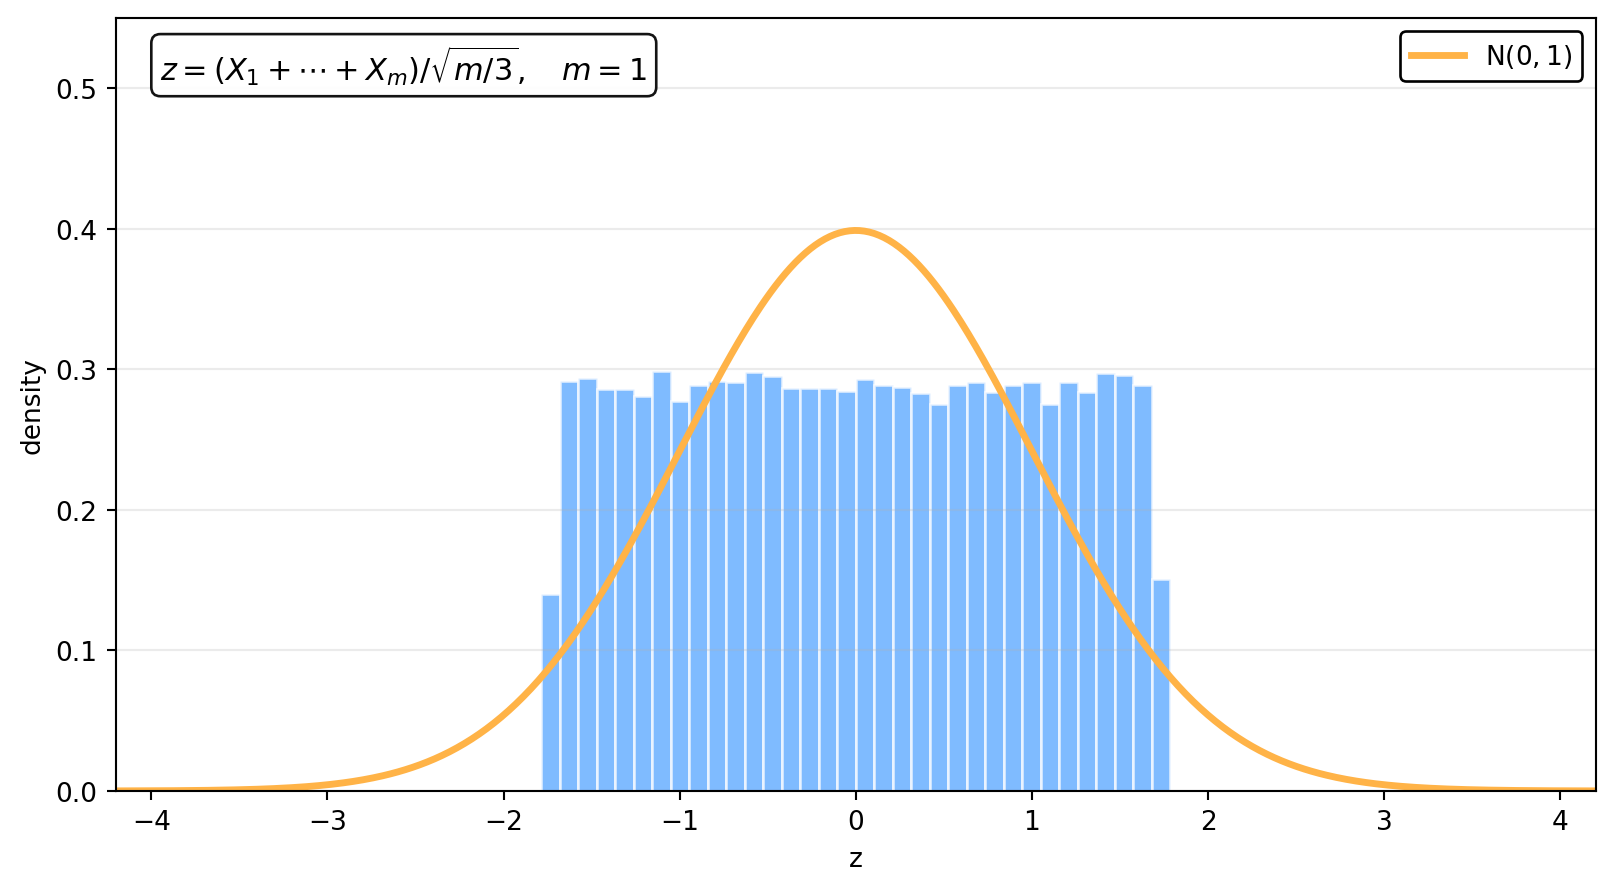
\includegraphics[keepaspectratio,alt={Нормированная сумма при m=1: исходная равномерная форма ещё совсем не похожа на гаусс.}]{chapters/../assets/figures/clt_uniform_sum_m1.png}}

\end{center}

\BookInlineFigureCaption{Нормированная сумма при \(m=1\): исходная равномерная форма ещё совсем
не похожа на гаусс.}

\end{bookfigurepanel}

\begin{bookfigurepanel}

\begin{center}

\pandocbounded{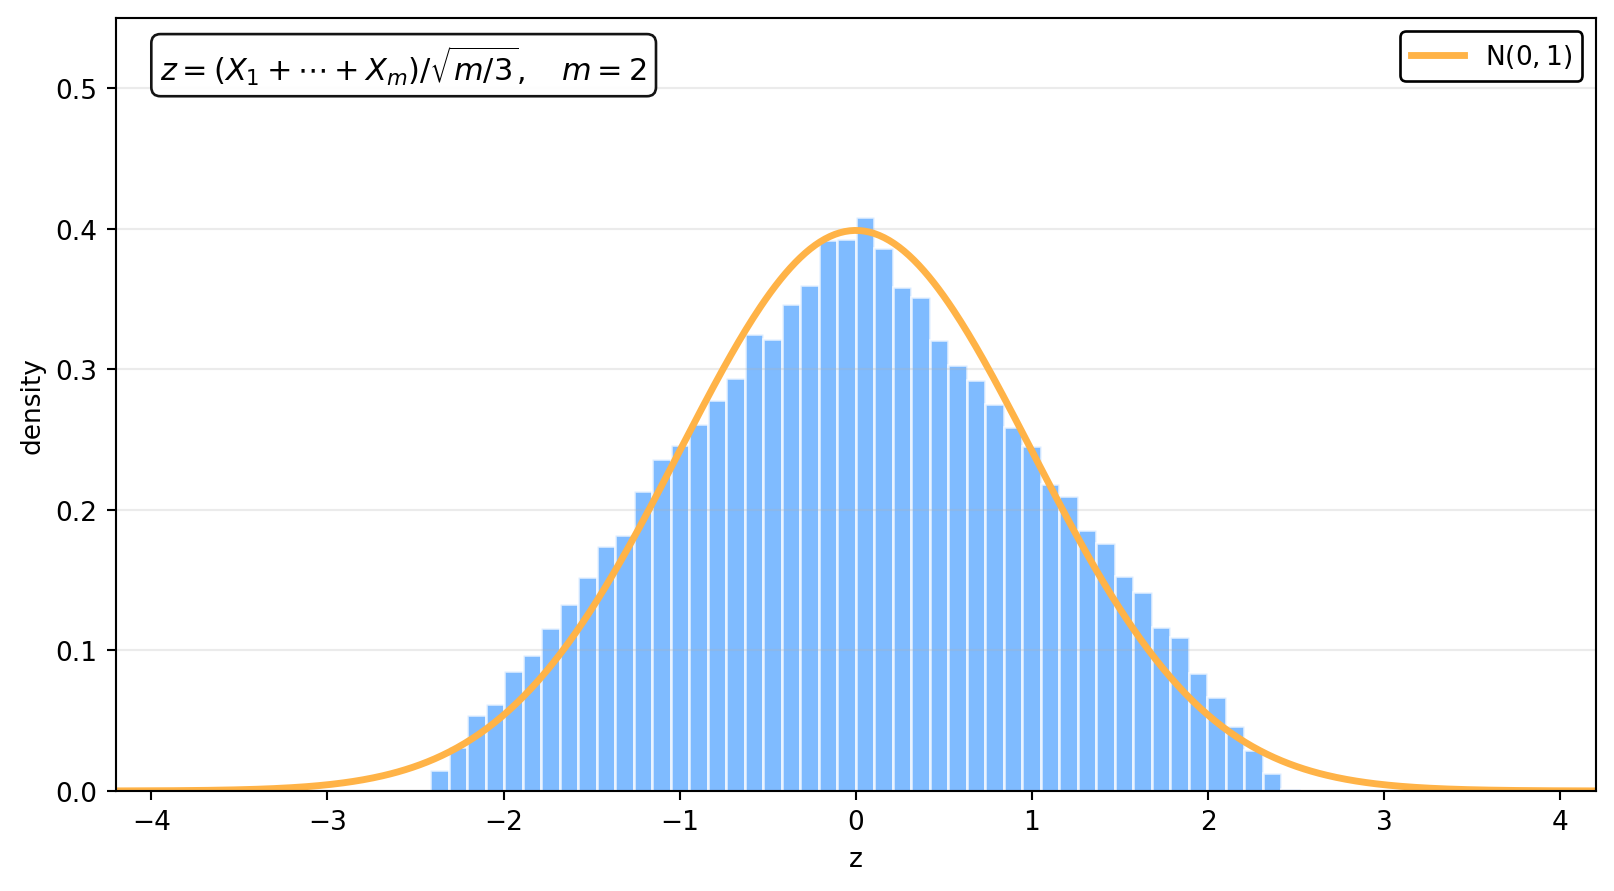
\includegraphics[keepaspectratio,alt={При m=2 возникает характерная треугольная форма.}]{chapters/../assets/figures/clt_uniform_sum_m2.png}}

\end{center}

\BookInlineFigureCaption{При \(m=2\) возникает характерная треугольная форма.}

\end{bookfigurepanel}

\begin{bookfigurepanel}

\begin{center}

\pandocbounded{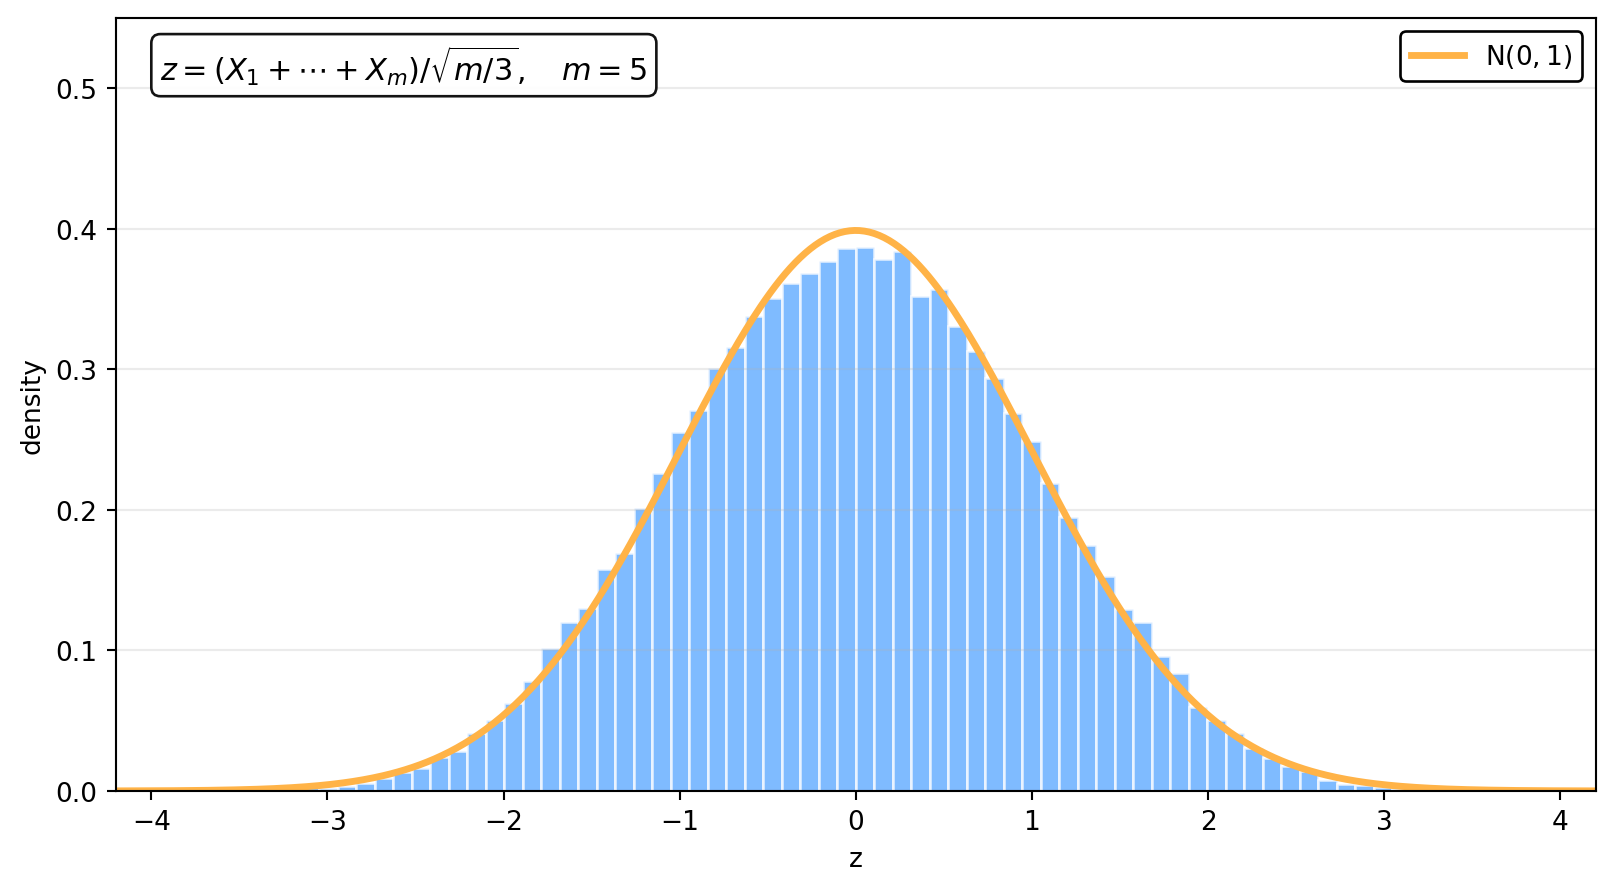
\includegraphics[keepaspectratio,alt={При m=5 нормированная сумма уже близка к стандартному нормальному распределению.}]{chapters/../assets/figures/clt_uniform_sum_m5.png}}

\end{center}

\BookInlineFigureCaption{При \(m=5\) нормированная сумма уже близка к стандартному нормальному
распределению.}

\end{bookfigurepanel}

\begin{bookfigurepanel}

\begin{center}

\pandocbounded{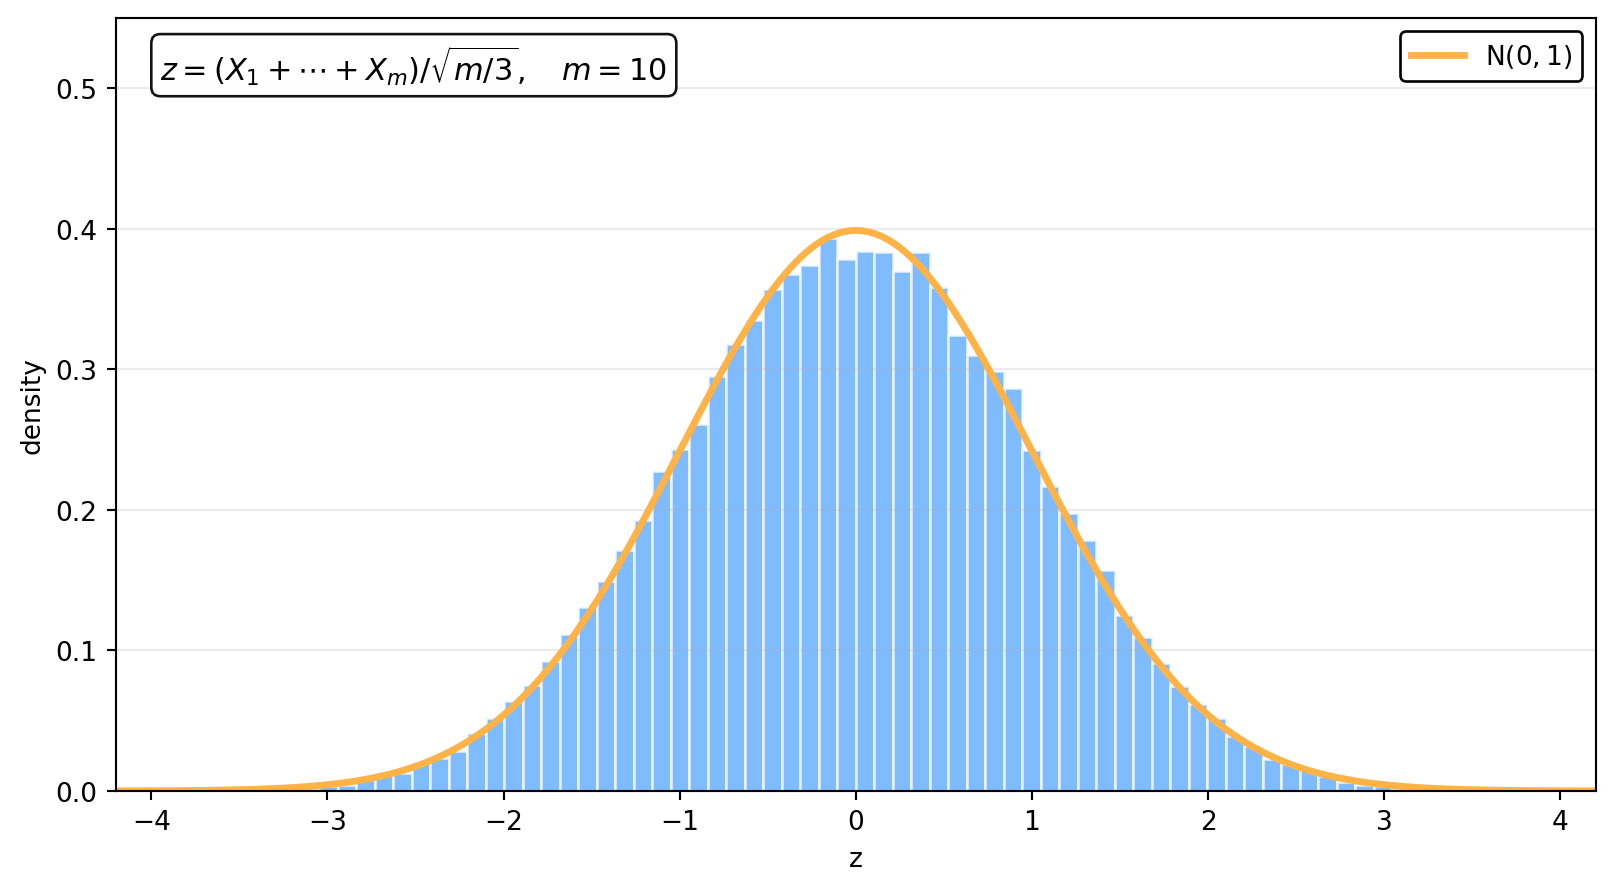
\includegraphics[keepaspectratio,alt={При m=10 различие между распределением суммы и стандартным гауссом визуально становится небольшим.}]{chapters/../assets/figures/clt_uniform_sum_m10.png}}

\end{center}

\BookInlineFigureCaption{При \(m=10\) различие между распределением суммы и стандартным гауссом
визуально становится небольшим.}

\end{bookfigurepanel}

Полное математическое доказательство центральной предельной теоремы
здесь не требуется. Для дальнейшего статистического анализа важен сам
результат и понимание того, какие свойства суммы приводят к появлению
нормального распределения.

\section{Гауссово
распределение}\label{ux433ux430ux443ux441ux441ux43eux432ux43e-ux440ux430ux441ux43fux440ux435ux434ux435ux43bux435ux43dux438ux435}

Центральная предельная теорема объясняет особую роль нормального
распределения: наблюдаемая величина часто складывается из большого числа
малых случайных вкладов. Именно с этим связана широкая роль
распределения Гаусса при описании ошибок измерений, интервалов и
объединения результатов.

\subsection{Одномерное нормальное
распределение}\label{ux43eux434ux43dux43eux43cux435ux440ux43dux43eux435-ux43dux43eux440ux43cux430ux43bux44cux43dux43eux435-ux440ux430ux441ux43fux440ux435ux434ux435ux43bux435ux43dux438ux435}

Плотность одномерного распределения Гаусса имеет вид: \[\boxed{
f(x;\mu,\sigma)
=
\frac{1}{\sigma\sqrt{2\pi}}
\exp\!\left[-\frac{(x-\mu)^2}{2\sigma^2}\right].
}\] Здесь \(\mu\) задаёт наиболее вероятное значение распределения
\(x\), а \(\sigma\) характеризует ширину распределения. Дисперсия равна
\(\sigma^2\), а нормировка удовлетворяет условию:
\[\int_{-\infty}^{+\infty}f(x;\mu,\sigma)\,dx=1.\]

\begin{bookfigurepanel}

\begin{center}

\pandocbounded{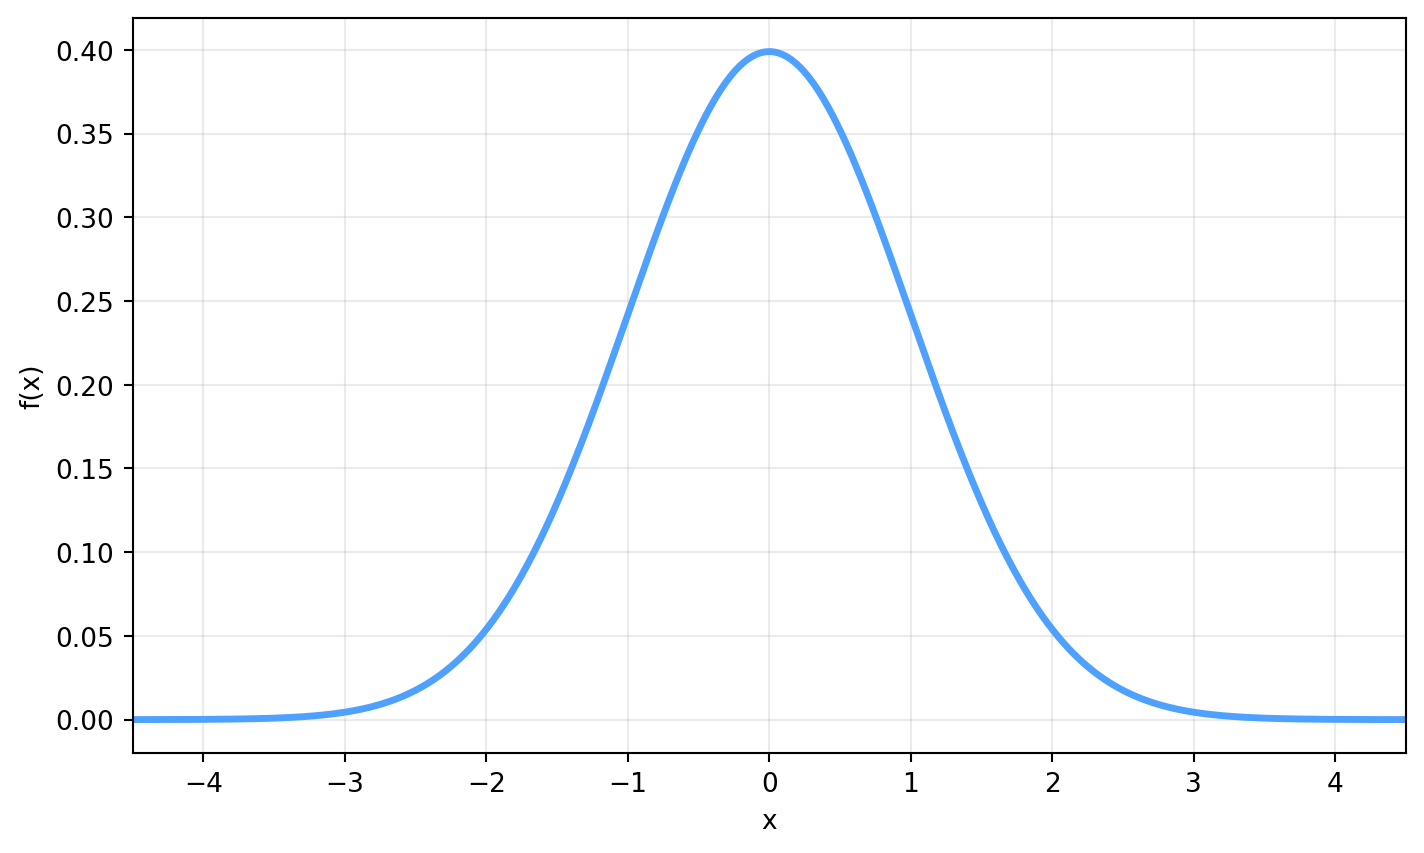
\includegraphics[keepaspectratio,alt={Стандартное нормальное распределение при \textbackslash mu=0 и \textbackslash sigma=1.}]{chapters/../assets/figures/gaussian_standard_density.png}}

\end{center}

\BookInlineFigureCaption{Стандартное нормальное распределение при \(\mu=0\) и \(\sigma=1\).}

\end{bookfigurepanel}

\subsection{Стандартизация}\label{ux441ux442ux430ux43dux434ux430ux440ux442ux438ux437ux430ux446ux438ux44f}

Если \[X\sim\mathrm{N}(\mu,\sigma),\] то после замены на величину:
\[Z=\frac{X-\mu}{\sigma}.\] получаем стандартное нормальное
распределение:

\begin{booknote}

\[\boxed{
Z\sim\mathrm{N}(0,1),
\qquad
f_Z(z)=\frac{1}{\sqrt{2\pi}}e^{-z^2/2}.
}\]

\end{booknote}

Такое преобразование переводит отклонение от среднего в единицы
стандартного отклонения \(\sigma\).

\section{Квантили стандартного нормального
распределения}\label{ux43aux432ux430ux43dux442ux438ux43bux438-ux441ux442ux430ux43dux434ux430ux440ux442ux43dux43eux433ux43e-ux43dux43eux440ux43cux430ux43bux44cux43dux43eux433ux43e-ux440ux430ux441ux43fux440ux435ux434ux435ux43bux435ux43dux438ux44f}

В лекции о случайных величинах и распределениях для
\(Z\sim\mathrm{N}(0,1)\) мы ввели кумулятивную функцию распределения:
\[\Phi(z)
=P(Z\le z)=\frac{1}{\sqrt{2\pi}}\int_{-\infty}^{z}e^{-t^2/2}\,dt=\frac12\left[1+\operatorname{erf}\!\left(\frac{z}{\sqrt2}\right)
\right].\] При \(z\to-\infty\) функция стремится к нулю, а при
\(z\to+\infty\) -- к единице.

\begin{booknote}

\textbf{Квантиль уровня} \(\beta\) стандартного нормального
распределения \(Z\sim\mathrm{N}(0,1)\) -- это число \(z_\beta\), для
которого выполняется следующее равенство:
\[\boxed{\Phi(z_\beta)=\beta.}\] Иными словами,
\[P(-\infty<Z\le z_\beta)=\beta.\]

\end{booknote}

Например, для \(\beta=0.90\) получаем \(z_\beta\approx1.282\), а для
\(\beta=0.95\) -- \(z_\beta\approx1.645\).

{\def\LTcaptype{none} % do not increment counter
\begin{longtable}[]{@{}cc@{}}
\toprule\noalign{}
Уровень \(\beta\) & \(z_\beta\) \\
\midrule\noalign{}
\endhead
\bottomrule\noalign{}
\endlastfoot
\(0.90\) & \(1.282\) \\
\(0.95\) & \(1.645\) \\
\(0.975\) & \(1.960\) \\
\(0.995\) & \(2.576\) \\
\end{longtable}
}

\begin{bookfigurepanel}

\begin{center}

\pandocbounded{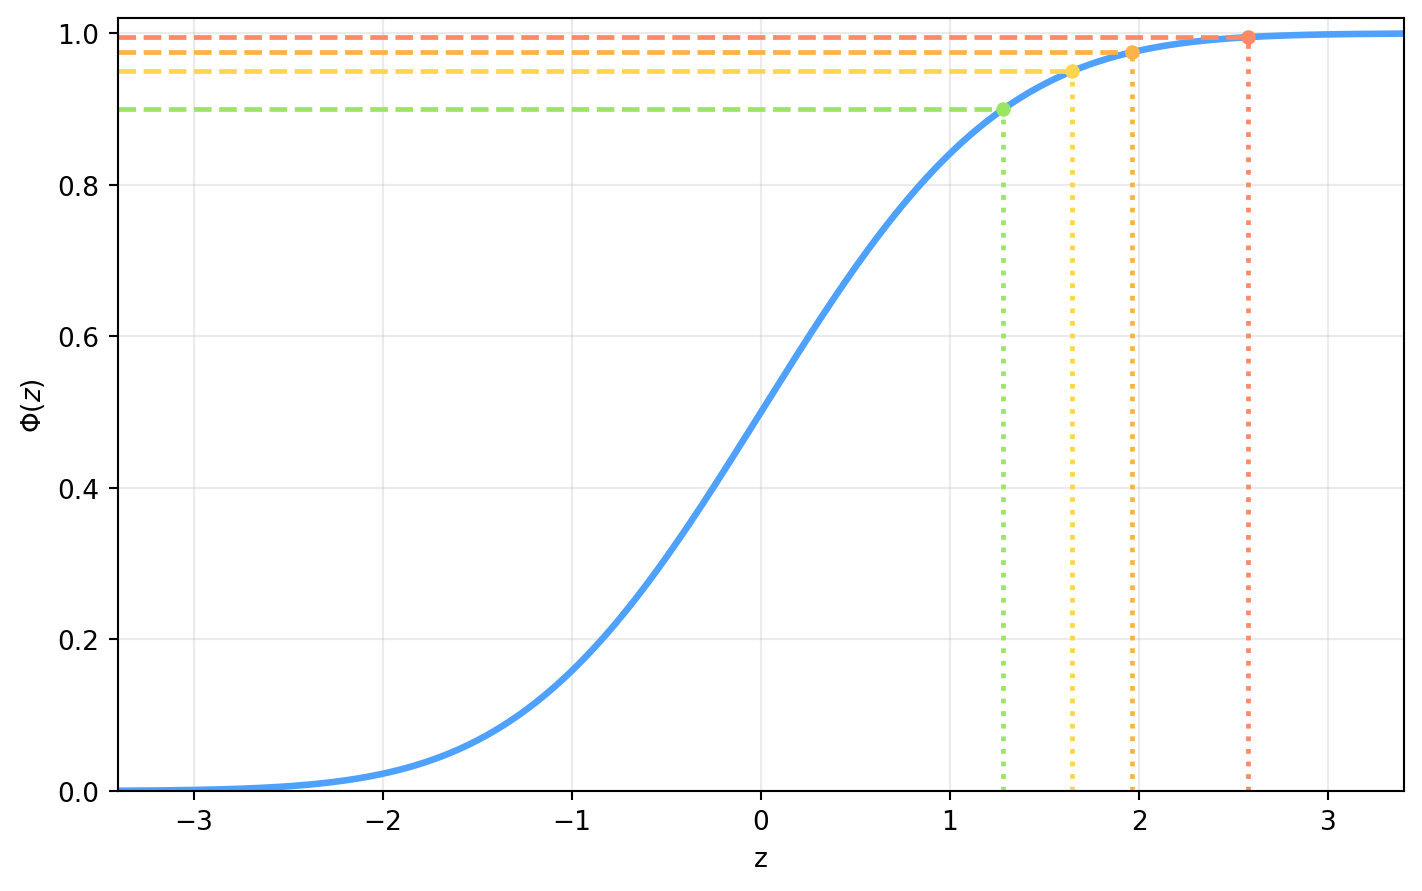
\includegraphics[keepaspectratio,alt={Кумулятивная функция стандартного нормального распределения и несколько уровней квантилей.}]{chapters/../assets/figures/normal_quantile_cdf.png}}

\end{center}

\BookInlineFigureCaption{Кумулятивная функция стандартного нормального распределения и несколько
уровней квантилей.}

\end{bookfigurepanel}

\section{Центральные
интервалы}\label{ux446ux435ux43dux442ux440ux430ux43bux44cux43dux44bux435-ux438ux43dux442ux435ux440ux432ux430ux43bux44b}

Односторонний квантиль задаёт область от \(-\infty\) до выбранной
границы. Для симметричного нормального распределения часто удобнее
использовать центральный интервал, одинаково отрезающий левый и правый
хвосты. Пусть вероятность попасть внутрь центральной области равна
\(\gamma\): \[P\!\left(
|Z|\le z_{(1+\gamma)/2}
\right)=\gamma.\] Если обозначить суммарную вероятность двух хвостов
через \[\alpha=1-\gamma,\] то критическая граница записывается как:
\[\boxed{z_{1-\alpha/2}}.\] При таком определении каждый хвост имеет
вероятность \(\alpha/2\).

\subsection{\texorpdfstring{Интервалы \(1\sigma\), \(2\sigma\) и
\(3\sigma\)}{Интервалы 1\textbackslash sigma, 2\textbackslash sigma и 3\textbackslash sigma}}\label{ux438ux43dux442ux435ux440ux432ux430ux43bux44b-1sigma-2sigma-ux438-3sigma}

Для гауссовского распределения особенно часто используются центральные
интервалы в единицах \(\sigma\):

\begin{itemize}
\tightlist
\item
  \(|X-\mu|<1\sigma\) содержит примерно \(68.3\%\) вероятности;
\item
  \(|X-\mu|<2\sigma\) содержит примерно \(95.4\%\);
\item
  \(|X-\mu|<3\sigma\) содержит примерно \(99.7\%\).
\end{itemize}

\begin{bookfigurepanel}

\begin{center}

\pandocbounded{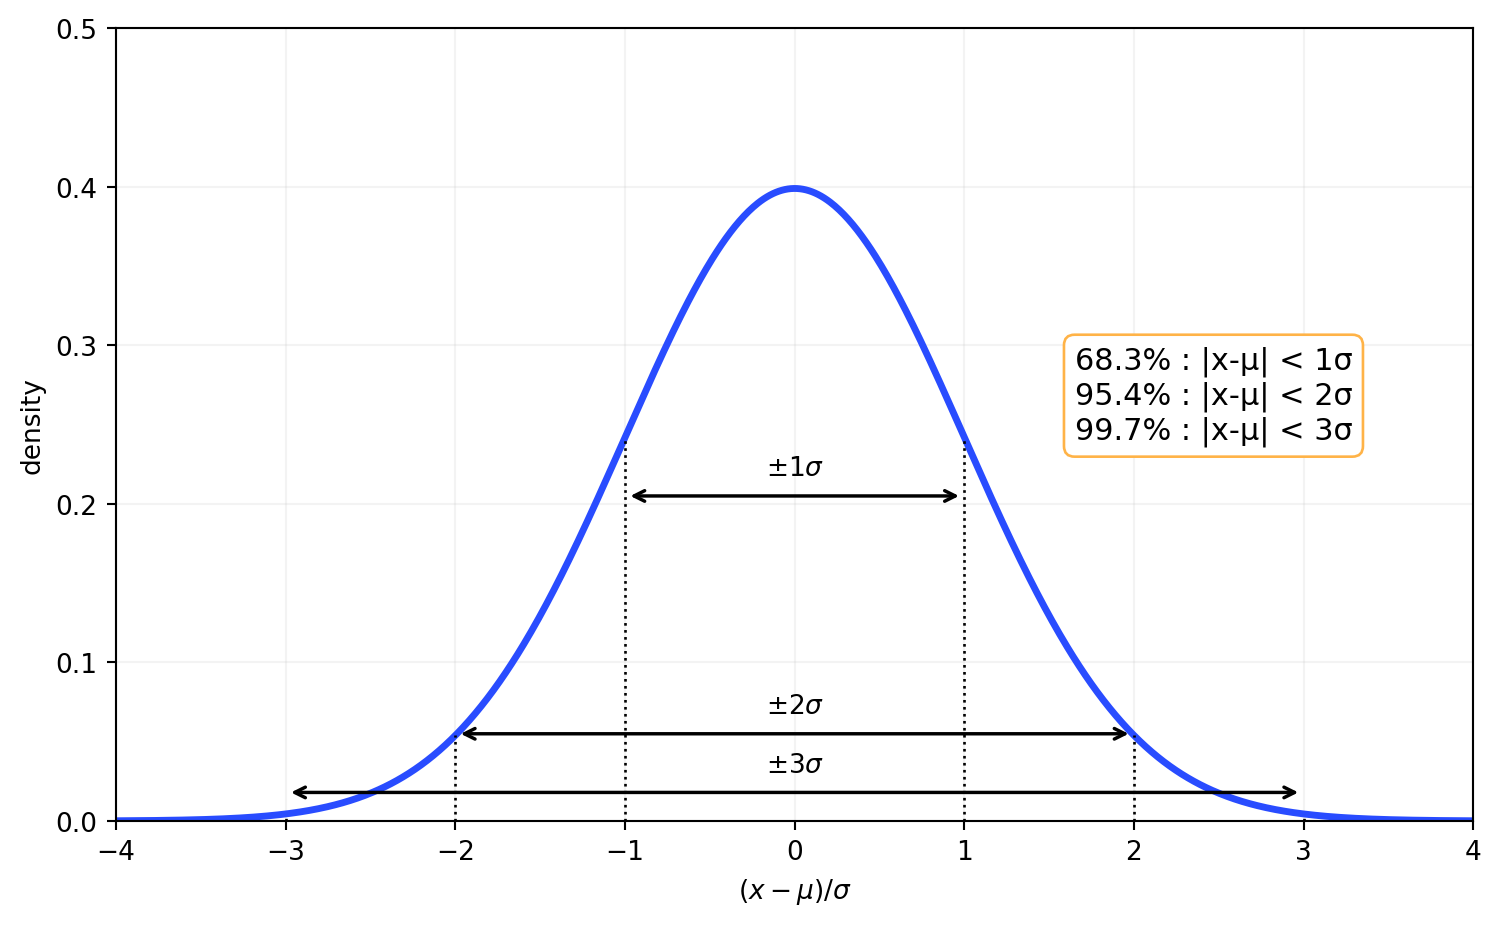
\includegraphics[keepaspectratio,alt={Центральные интервалы \textbackslash pm1\textbackslash sigma, \textbackslash pm2\textbackslash sigma и \textbackslash pm3\textbackslash sigma стандартного нормального распределения.}]{chapters/../assets/figures/normal_central_intervals.png}}

\end{center}

\BookInlineFigureCaption{Центральные интервалы \(\pm1\sigma\), \(\pm2\sigma\) и \(\pm3\sigma\)
стандартного нормального распределения.}

\end{bookfigurepanel}

\begin{booknote}

Одна «сигма» в таком центральном интервале означает одну \(\sigma\)
вправо и одну \(\sigma\) влево от среднего. Полная ширина интервала
\(\pm1\sigma\) равна \(2\sigma\).

\end{booknote}

Вероятности \(68\%\), \(95\%\) и даже \(99.7\%\) в физике соответствуют
лишь примерно одной, двум и трём стандартным сигмам. Для заявления об
открытии обычно требуется статистическая значимость не меньше пяти
стандартных отклонений: такой критерий возник как практический результат
многолетней экспериментальной работы, когда менее значимые отклонения
неоднократно оказывались флуктуациями.

\section{Совместимость двух
измерений}\label{ux441ux43eux432ux43cux435ux441ux442ux438ux43cux43eux441ux442ux44c-ux434ux432ux443ux445-ux438ux437ux43cux435ux440ux435ux43dux438ux439}

Пусть два независимых измерения одной и той же величины имеют вид:
\[x_1\pm\sigma_1,
\qquad
x_2\pm\sigma_2.\] Сравнивать только центральные значения недостаточно.
Разность может выглядеть большой, но быть обычной флуктуацией при
больших неопределённостях, или наоборот --- небольшая разность может
оказаться очень значимой, если ошибки малы.

Рассмотрим две пары значений: \[1.0\pm0.5,
\qquad
2.0\pm0.5,\] и \[1.010\pm0.001,
\qquad
1.020\pm0.001.\]

\subsection{Распределение
разности}\label{ux440ux430ux441ux43fux440ux435ux434ux435ux43bux435ux43dux438ux435-ux440ux430ux437ux43dux43eux441ux442ux438}

Введём случайную величину: \[D=X_1-X_2.\] Если оба измерения оценивают
одну и ту же величину \(\mu\), то при гипотезе совместимости:
\[\mathbb{E}[D]=\mathbb{E}[X_1-X_2]=\mu-\mu=0.\]

\begin{bookderivation}

\subsubsection{Дисперсия разности и наблюдаемая
значимость}\label{ux434ux438ux441ux43fux435ux440ux441ux438ux44f-ux440ux430ux437ux43dux43eux441ux442ux438-ux438-ux43dux430ux431ux43bux44eux434ux430ux435ux43cux430ux44f-ux437ux43dux430ux447ux438ux43cux43eux441ux442ux44c}

Для разности

\[D=X_1-X_2\]

дисперсия равна

\[\mathrm{Var}(D)
=\mathrm{Var}(X_1-X_2)=
\sigma_1^2+
\sigma_2^2-
2\,\mathrm{cov}(X_1,X_2).\]

Если измерения независимы, то

\[\mathrm{cov}(X_1,X_2)=0,\]

и тогда

\[\boxed{
\sigma_D^2=\sigma_1^2+\sigma_2^2,
\qquad
\sigma_D=\sqrt{\sigma_1^2+\sigma_2^2}.
}\]

Если ошибки гауссовы, то:

\[D\sim\mathrm{N}(0,\sigma_D),\]

а нормированная величина

\[Z=\frac{D}{\sigma_D}\]

имеет стандартное нормальное распределение. Для наблюдённых значений
получаем:

\[\boxed{
z_{\mathrm{obs}}
=
\frac{x_1-x_2}{\sqrt{\sigma_1^2+\sigma_2^2}}.
}\quad\blacksquare\]

\end{bookderivation}

\subsection{Правило проверки совместимости двух
измерений}\label{ux43fux440ux430ux432ux438ux43bux43e-ux43fux440ux43eux432ux435ux440ux43aux438-ux441ux43eux432ux43cux435ux441ux442ux438ux43cux43eux441ux442ux438-ux434ux432ux443ux445-ux438ux437ux43cux435ux440ux435ux43dux438ux439}

Выбирается центральная область совместимости с вероятностью \(\gamma\).
Ей соответствует \[\alpha=1-\gamma\] и критическая граница \[\boxed{
c=z_{(1+\gamma)/2}=z_{1-\alpha/2}.
}\] Например, при \[\gamma=0.90,
\qquad
\alpha=0.10,\] получаем \[c=z_{0.95}\approx1.64.\] Правило проверки
имеет вид: \[|z_{\mathrm{obs}}|\le c\] --- совместимость не отвергается.
Если \[|z_{\mathrm{obs}}|>c,\] наблюдаемая разность попадает в хвост
стандартного нормального распределения и измерения считаются
несовместимыми на выбранном уровне значимости \(\alpha\).

Обратите внимание: утверждение о совместимости всегда должно
сопровождаться выбранным уровнем \(\gamma\) или, эквивалентно,
\(\alpha\).

\begin{bookfigurepanel}

\begin{center}

\pandocbounded{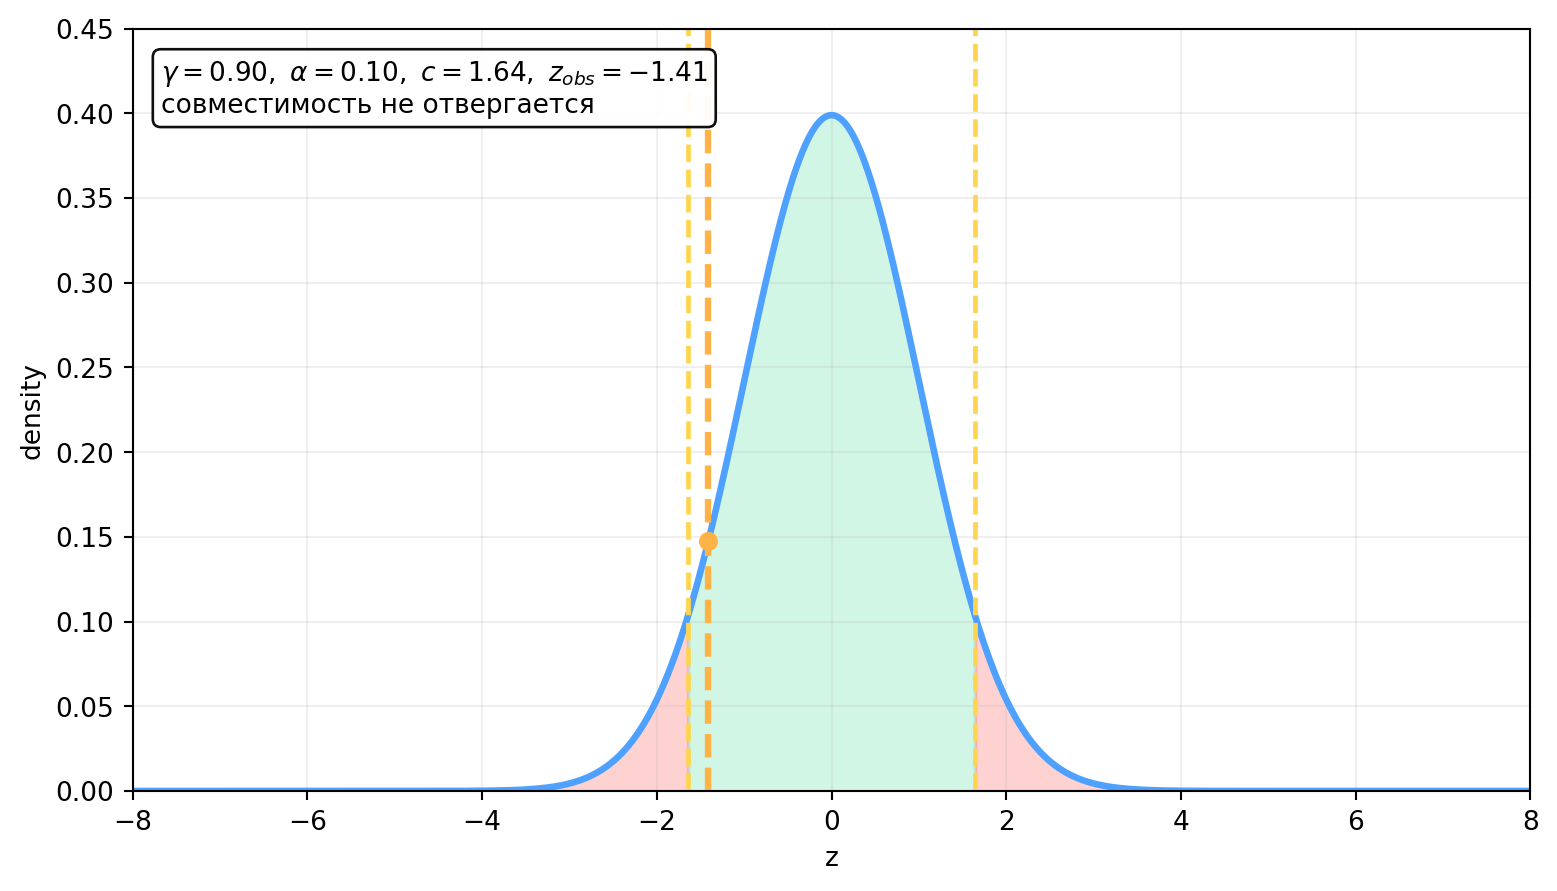
\includegraphics[keepaspectratio,alt={Пример A при центральной области \textbackslash gamma=0.90: z\_\{\textbackslash mathrm\{obs\}\}=-1.41 остаётся внутри критических границ, поэтому совместимость не отвергается.}]{chapters/../assets/figures/compatibility_example_a.png}}

\end{center}

\BookInlineFigureCaption{Пример A при центральной области \(\gamma=0.90\):
\(z_{\mathrm{obs}}=-1.41\) остаётся внутри критических границ, поэтому
совместимость не отвергается.}

\end{bookfigurepanel}

\begin{bookfigurepanel}

\begin{center}

\pandocbounded{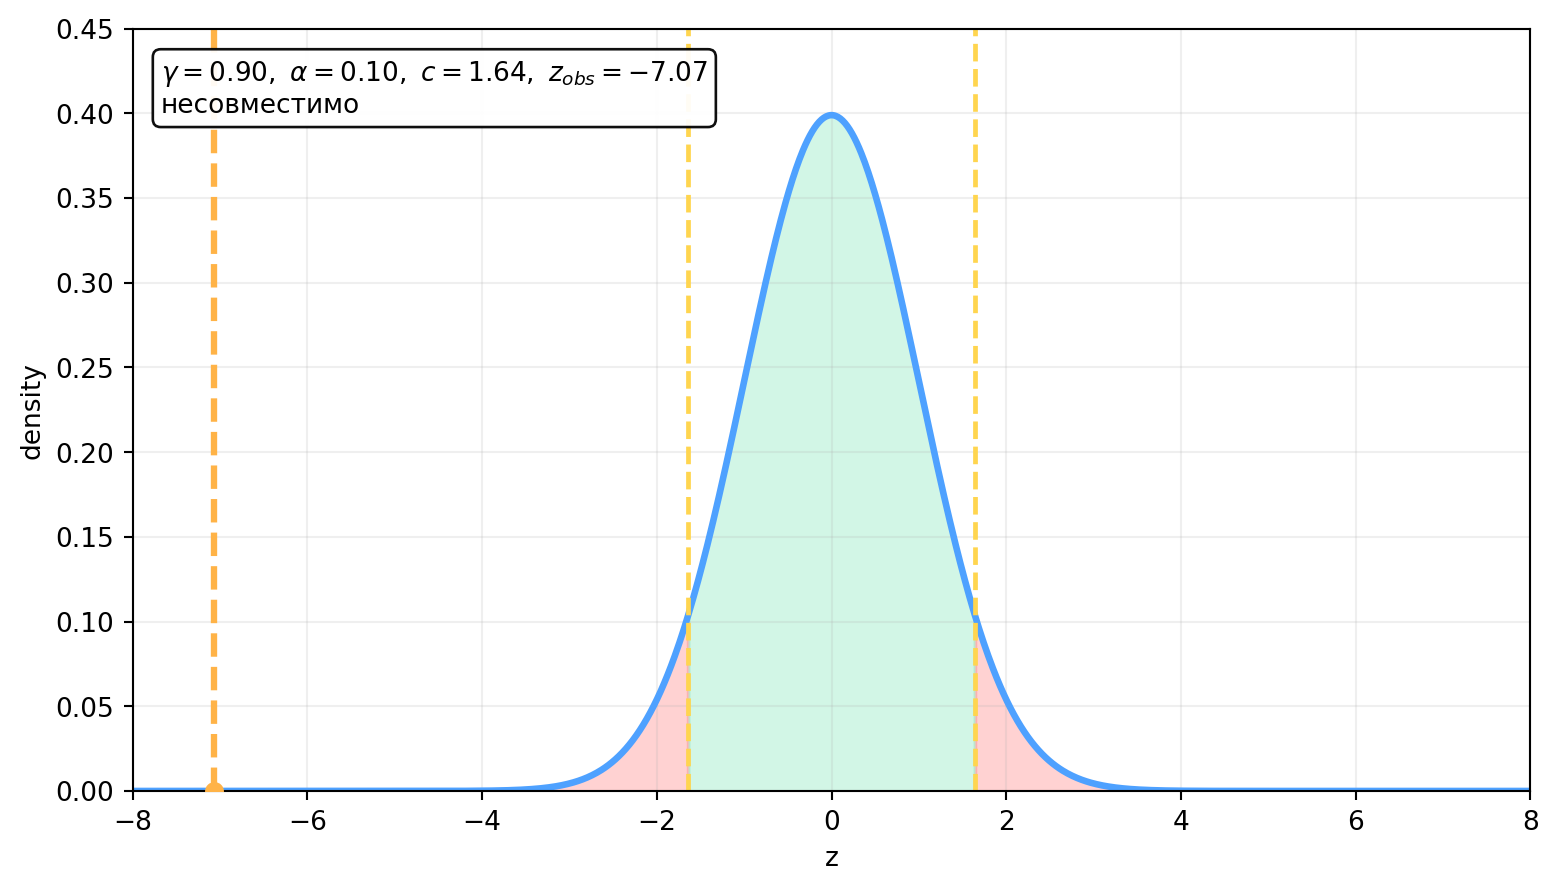
\includegraphics[keepaspectratio,alt={Пример B при той же центральной области: z\_\{\textbackslash mathrm\{obs\}\}=-7.07 находится далеко в хвосте, поэтому измерения несовместимы.}]{chapters/../assets/figures/compatibility_example_b.png}}

\end{center}

\BookInlineFigureCaption{Пример B при той же центральной области: \(z_{\mathrm{obs}}=-7.07\)
находится далеко в хвосте, поэтому измерения несовместимы.}

\end{bookfigurepanel}

\subsection{Два численных
примера}\label{ux434ux432ux430-ux447ux438ux441ux43bux435ux43dux43dux44bux445-ux43fux440ux438ux43cux435ux440ux430}

Для первой пары \[1.0\pm0.5,
\qquad
2.0\pm0.5\] получаем
\[z_{\mathrm{obs}}=\frac{1.0-2.0}{\sqrt{0.5^2+0.5^2}}\approx -1.41.\]
При \(\gamma=0.90\) критическая граница составляет примерно \(1.64\),
так что \(|z_{\mathrm{obs}}|<1.64\): совместимость не отвергается.

Для второй пары \[1.010\pm0.001,
\qquad
1.020\pm0.001\] имеем: \[
z_{\mathrm{obs}}=\frac{1.010-1.020}{\sqrt{0.001^2+0.001^2}}\approx -7.07.\]
Хотя центральные значения здесь расположены гораздо ближе друг к другу,
неопределённости настолько малы, что нормированная разность очень
велика. Эти измерения сильно несовместимы.

\begin{booknote}

При сравнении измерений важна не абсолютная разность центральных
значений, а \textbf{разность в единицах совместной неопределённости}.
Маленькое численное отличие может быть статистически значимым, если
ошибки ещё меньше.

\end{booknote}

\begin{bookchaptersummary}[Итоги главы]

\begin{itemize}
\tightlist
\item
  Псевдослучайные генераторы позволяют получать на компьютере выборки,
  статистически ведущие себя как случайные.
\item
  Для независимой суммы дисперсии складываются, а ковариационные члены
  исчезают.
\item
  Центральная предельная теорема утверждает, что центрированная и
  нормированная сумма большого числа независимых вкладов с конечными
  дисперсиями стремится к стандартному нормальному распределению.
\item
  Стандартизация \(Z=(X-\mu)/\sigma\) переводит нормальную величину к
  распределению \(\mathrm{N}(0,1)\).
\item
  Квантили и центральные интервалы связывают вероятности с числом
  стандартных отклонений.
\item
  Совместимость независимых измерений проверяется по нормированной
  разности \(z_{\mathrm{obs}}\).
\end{itemize}

\end{bookchaptersummary}

\section{Материалы
курса}\label{ux43cux430ux442ux435ux440ux438ux430ux43bux44b-ux43aux443ux440ux441ux430-1}

\begin{itemize}
\tightlist
\item
  \href{https://neutrinohit.github.io/statistical-analysis-course/ru/slides/03_central_limit_theorem.html}{Слайды
  лекции}
\item
  \href{https://neutrinohit.github.io/statistical-analysis-course/ru/slides/exercises/03_central_limit_theorem_exercises.html}{Задачи}
\end{itemize}

\chapter{Когда не возникает гауссового
распределения}\label{ux43aux43eux433ux434ux430-ux43dux435-ux432ux43eux437ux43dux438ux43aux430ux435ux442-ux433ux430ux443ux441ux441ux43eux432ux43eux433ux43e-ux440ux430ux441ux43fux440ux435ux434ux435ux43bux435ux43dux438ux44f}

\begin{bookchapteropening}[Главная мысль]

Большое число наблюдений само по себе не гарантирует распределение
Гаусса в предельном случае. Центральная предельная теорема опирается на
независимость вкладов, конечность их дисперсий, отсутствие доминирующих
слагаемых и линейное суммирование. Тяжёлые хвосты, корреляции и
систематические ошибки, смеси разных классов событий и нелинейные
преобразования могут сохранять негауссову форму или дополнительную
ширину даже при очень большой статистике.

\end{bookchapteropening}

\section{План
главы}\label{ux43fux43bux430ux43d-ux433ux43bux430ux432ux44b-3}

\begin{itemize}
\tightlist
\item
  Где в центральной предельной теореме спрятаны ограничения
\item
  Распределение Коши и отсутствие сужения среднего
\item
  Энергетические потери и распределение Ландау
\item
  Коррелированные слагаемые и систематическая ошибка
\item
  Смесь распределений и скрытые классы событий
\item
  Пример жидкого сцинтиллятора
\item
  Отношение случайных величин
\item
  Практическая проверка применимости приближения Гаусса
\end{itemize}

\section{Когда центральная предельная теорема требует
осторожности}\label{ux43aux43eux433ux434ux430-ux446ux435ux43dux442ux440ux430ux43bux44cux43dux430ux44f-ux43fux440ux435ux434ux435ux43bux44cux43dux430ux44f-ux442ux435ux43eux440ux435ux43cux430-ux442ux440ux435ux431ux443ux435ux442-ux43eux441ux442ux43eux440ux43eux436ux43dux43eux441ux442ux438}

В главе про ЦПТ было показано, как сумма бесконечного числа независимых
вкладов описывается гауссовым распределением. Но в реальной жизни оно не
всегда возникает. Рассмотрим сумму: \[S_n=\sum_{i=1}^{n}X_i.\] Если
случайные величины независимы, имеют конечные средние и дисперсии:
\[\mathbb{E}[X_i]=\mu_i,
\qquad
\mathrm{Var}(X_i)=\sigma_i^2<\infty,\] то нормированная сумма \[Z_n=
\frac{S_n-\mathbb{E}[S_n]}
{\sqrt{\mathrm{Var}(S_n)}}\] при выполнении необходимых условий
стремится к стандартному нормальному распределению. Для одинаково
распределённых величин с \[\mathbb{E}[X_i]=\mu,
\qquad
\mathrm{Var}(X_i)=\sigma^2\] эту запись удобно переписать как: \[\boxed{
Z_n=
\frac{S_n/n-\mu}{\sigma/\sqrt n}.
}\] Среднее \(S_n/n\) стремится к \(\mu\), а характерный масштаб его
статистических отклонений имеет порядок \(\sigma/\sqrt n\). Тогда
\(Z_n\) стремится к стандартному гауссу при \(n \rightarrow \infty\):
\[\lim_{n\rightarrow\infty}Z_n\Rightarrow N(0,1).\]

\subsection{Где спрятаны
условия}\label{ux433ux434ux435-ux441ux43fux440ux44fux442ux430ux43dux44b-ux443ux441ux43bux43eux432ux438ux44f}

\begin{booknote}

Для гауссова предела необходимо выполнение нескольких условий:

\begin{itemize}
\tightlist
\item
  сумма должна состоять из большого числа малых вкладов;
\item
  ни один отдельный вклад не должен доминировать над остальными;
\item
  распределения не должны иметь бесконечно тяжёлых хвостов;
\item
  между слагаемыми должны отсутствовать корреляций;
\item
  нужно рассматривать именно сумму, а не произвольную нелинейную функцию
  суммы.
\end{itemize}

\end{booknote}

Напомним, что для суммы \(S_n\) дисперсия имеет следующий общий вид:
\[\mathrm{Var}(S_n)
=
\sum_i\mathrm{Var}(X_i)
+2\sum_{i<j}\mathrm{cov}(X_i,X_j).\] Если ковариации равны нулю,
дисперсии просто складываются. Если ковариации велики, само увеличение
числа слагаемых уже ничего не гарантирует. Если дисперсия отдельного
вклада не существует, стандартная нормировка через \(\sqrt n\) также
теряет привычный смысл.

\section{Распределение Коши и центральная предельная
теорема}\label{ux440ux430ux441ux43fux440ux435ux434ux435ux43bux435ux43dux438ux435-ux43aux43eux448ux438-ux438-ux446ux435ux43dux442ux440ux430ux43bux44cux43dux430ux44f-ux43fux440ux435ux434ux435ux43bux44cux43dux430ux44f-ux442ux435ux43eux440ux435ux43cux430}

Стандартное распределение Коши имеет плотность:
\[f(x)=\frac{1}{\pi}\frac{1}{1+x^2}.\] Его кумулятивная функция
распределения (CDF): \[F(x)=\frac12+\frac{1}{\pi}\arctan x.\] Обратная
CDF позволяет генерировать случайные значения с таким распределением из
равномерно распределённой величины \(u\) : \[F^{-1}(u)
=
\tan\!\left[\pi\left(u-\frac12\right)\right].\]

\begin{booknote}

Обратите внимание, у распределения Коши расходятся моменты, необходимые
для обычной центральной предельной теоремы. В частности,
\[\mathbb{E}[|X|]=\infty,
\qquad
\mathbb{E}[X^2]=\infty.\] Среднее и дисперсия в обычном смысле не
определены.

\end{booknote}

\subsection{Среднее Коши не сужается с ростом числа
наблюдений}\label{ux441ux440ux435ux434ux43dux435ux435-ux43aux43eux448ux438-ux43dux435-ux441ux443ux436ux430ux435ux442ux441ux44f-ux441-ux440ux43eux441ux442ux43eux43c-ux447ux438ux441ux43bux430-ux43dux430ux431ux43bux44eux434ux435ux43dux438ux439}

Пусть случайные величины \[X_1,\ldots,X_n\sim\mathrm{Cauchy}(0,1)\]
независимы. Тогда, как мы видели в главе про характеристические функции,
их сумма \[S_n=\sum_{i=1}^{n}X_i\] имеет распределение:
\[S_n\sim\mathrm{Cauchy}(0,n).\] После деления на \(n\) масштаб снова
становится единичным: \[\boxed{
\frac{S_n}{n}\sim\mathrm{Cauchy}(0,1).
}\] Это означает, что распределение среднего не сужается при увеличении
\(n\). В отличие от обычного случая с конечной дисперсией, накопление
всё большего числа случайных величин Коши не превращает среднее в узкий
гауссовский пик.

\begin{bookfigurepanel}

\begin{center}

\pandocbounded{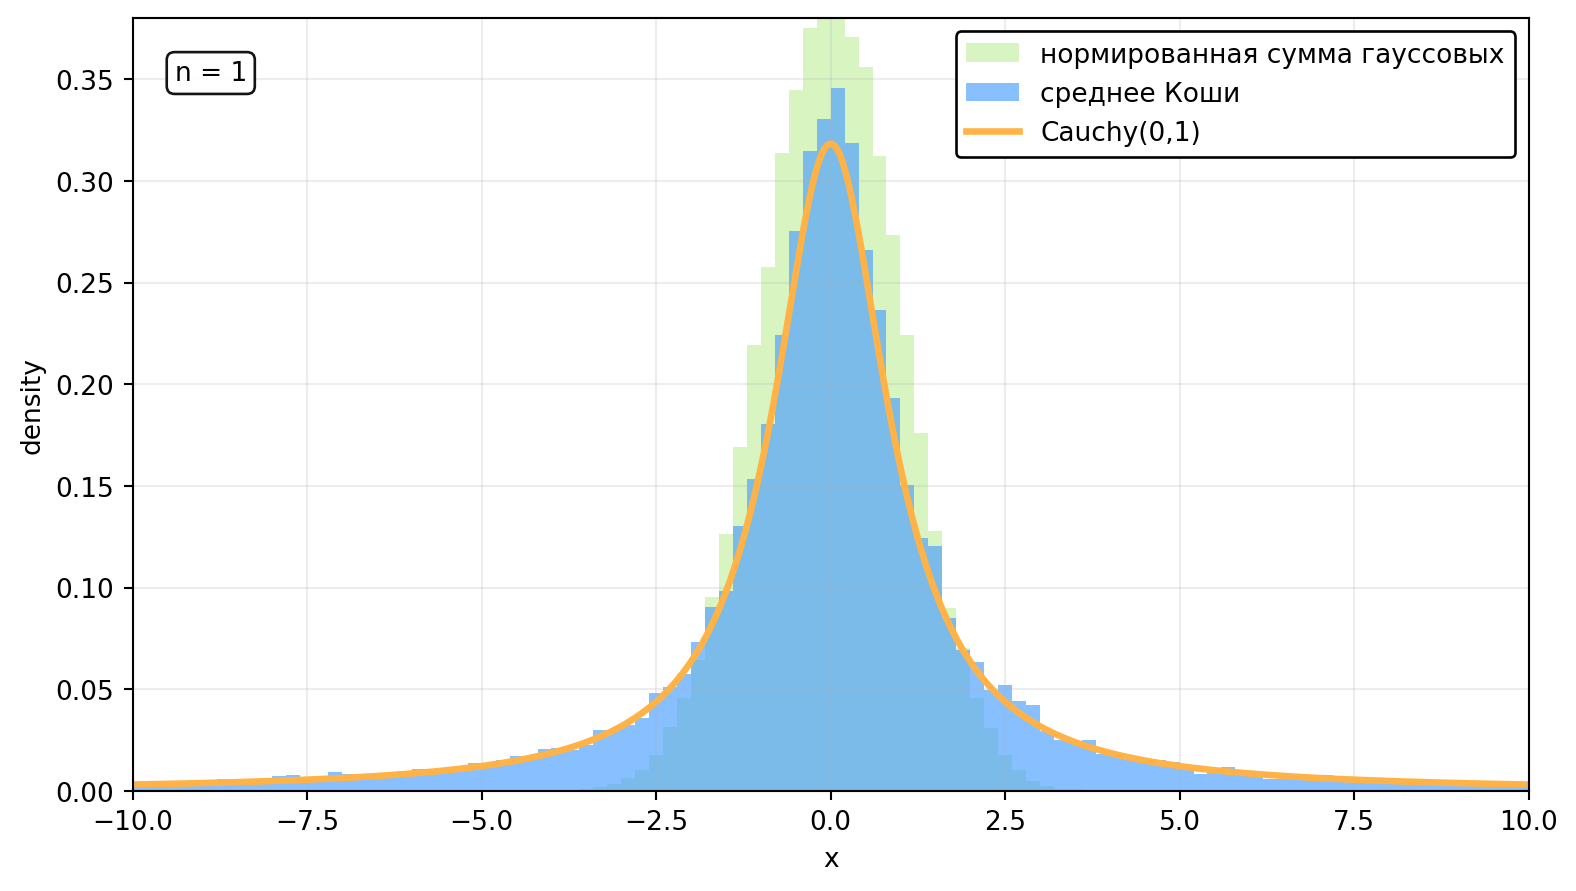
\includegraphics[keepaspectratio,alt={При n=1 распределение среднего Коши совпадает со стандартным распределением Коши. Для сравнения показана нормированная сумма гауссовых величин.}]{chapters/../assets/figures/cauchy_mean_n1.png}}

\end{center}

\BookInlineFigureCaption{При \(n=1\) распределение среднего Коши совпадает со стандартным
распределением Коши. Для сравнения показана нормированная сумма
гауссовых величин.}

\end{bookfigurepanel}

\begin{bookfigurepanel}

\begin{center}

\pandocbounded{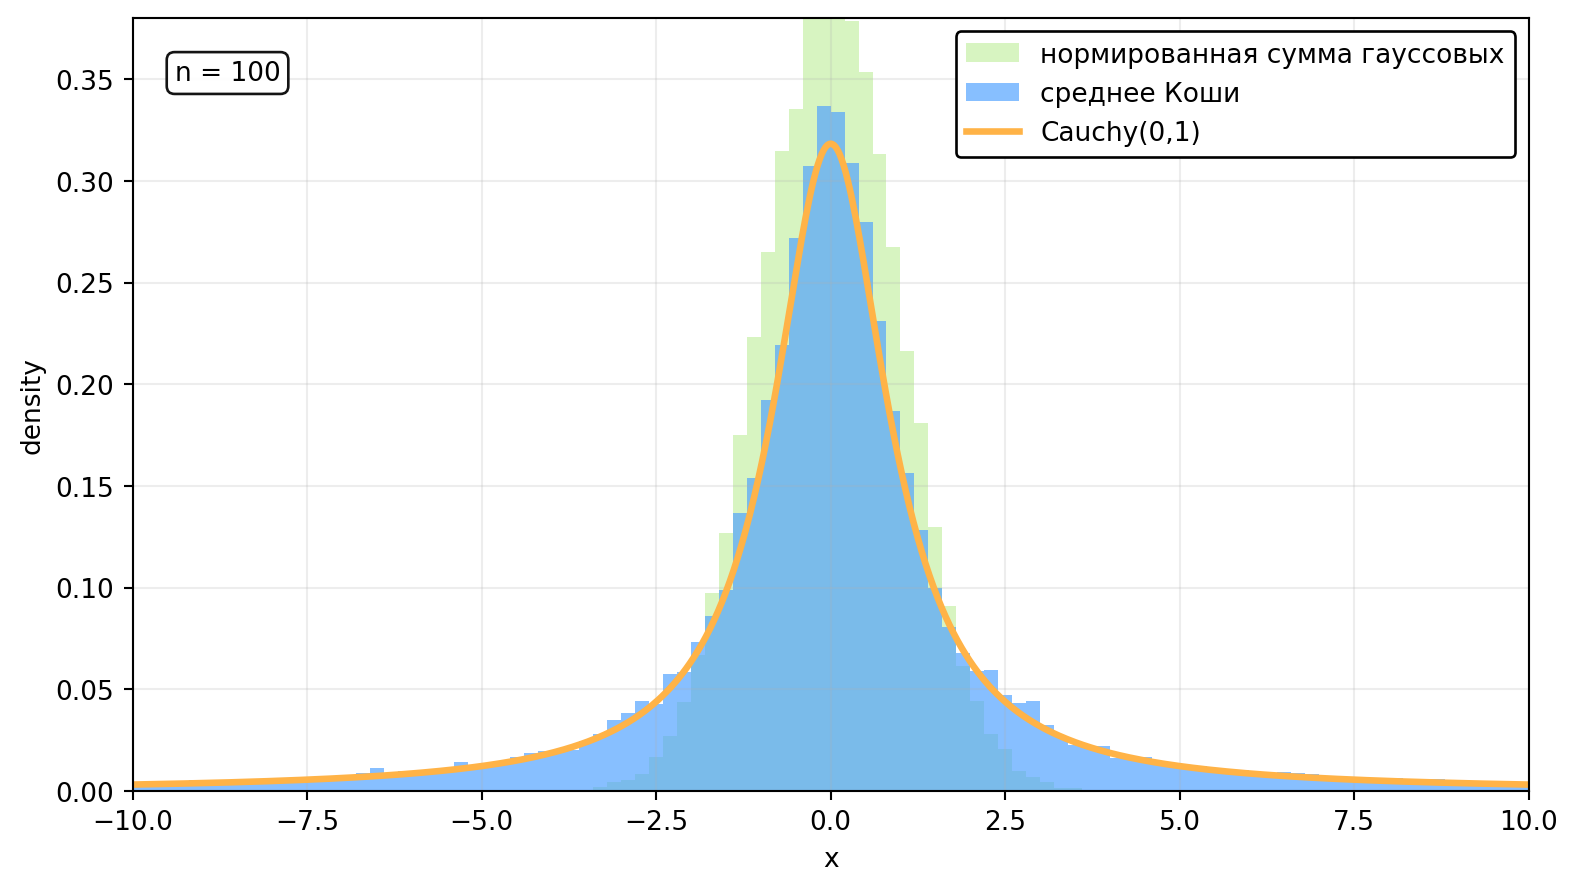
\includegraphics[keepaspectratio,alt={Даже при n=100 среднее Коши не сужается: синяя гистограмма остаётся распределением Коши, тогда как нормированная сумма гауссовых величин сохраняет нормальную форму.}]{chapters/../assets/figures/cauchy_mean_n100.png}}

\end{center}

\BookInlineFigureCaption{Даже при \(n=100\) среднее Коши не сужается: синяя гистограмма остаётся
распределением Коши, тогда как нормированная сумма гауссовых величин
сохраняет нормальную форму.}

\end{bookfigurepanel}

В физике высоких энергий распределение Коши известно как кривая
Брейта-Вигнера и используется при описании резонансов -- нестабильных
частиц, проявляющихся как пики в спектрах инвариантной массы.

Возникает естественный вопрос: если среднее Коши не сужается, означает
ли это, что накопление данных бесполезно? Такой вывод неверен. Ответ
требует перехода от простого среднего к задаче оценивания параметров
распределения, которая рассматривается отдельно.

\section{Энергетические потери в тонком слое
вещества}\label{ux44dux43dux435ux440ux433ux435ux442ux438ux447ux435ux441ux43aux438ux435-ux43fux43eux442ux435ux440ux438-ux432-ux442ux43eux43dux43aux43eux43c-ux441ux43bux43eux435-ux432ux435ux449ux435ux441ux442ux432ux430}

Заряженная частица теряет энергию в веществе во множестве актов
ионизации и возбуждения. Полную потерю энергии можно описать как сумму:
\[\Delta=\omega_1+\omega_2+\cdots+\omega_N.\] На первый взгляд такая
запись напоминает условия центральной предельной теоремы. Существенное
отличие состоит в том, что отдельные передачи энергии \(\omega_a\) не
обязаны быть одинаково малыми. Редкий акт может передать электрону
большую энергию и заметно изменить всю сумму. Такие высокоэнергичные
электроны называют \(\delta\)-электронами.

\subsection{Медленно убывающий хвост от редких больших передач
энергии}\label{ux43cux435ux434ux43bux435ux43dux43dux43e-ux443ux431ux44bux432ux430ux44eux449ux438ux439-ux445ux432ux43eux441ux442-ux43eux442-ux440ux435ux434ux43aux438ux445-ux431ux43eux43bux44cux448ux438ux445-ux43fux435ux440ux435ux434ux430ux447-ux44dux43dux435ux440ux433ux438ux438}

Для быстрой заряженной частицы сечение передачи энергии электрону имеет
приближённый вид: \[\frac{d\sigma}{d\omega}\propto\frac{1}{\omega^2}.\]

\begin{bookderivation}

\subsubsection{Вероятность большой передачи
энергии}\label{ux432ux435ux440ux43eux44fux442ux43dux43eux441ux442ux44c-ux431ux43eux43bux44cux448ux43eux439-ux43fux435ux440ux435ux434ux430ux447ux438-ux44dux43dux435ux440ux433ux438ux438}

Вероятность передачи энергии больше некоторого порога \(W\) оценивается
интегралом: \[P(\omega>W)
\propto
\int_W^{W_{\max}}\frac{d\omega}{\omega^2}.\] Интегрирование даёт:
\[P(\omega>W)\propto
\left[-\frac{1}{\omega}\right]_{W}^{W_{\max}}=
\frac{1}{W}-\frac{1}{W_{\max}}.\] Если \(W_{\max}\) достаточно велик по
сравнению с рассматриваемым \(W\), вторым членом можно пренебречь:
\[\boxed{
P(\omega>W)\propto\frac{1}{W}.
}\quad\blacksquare\]

\end{bookderivation}

Хвост \(1/W\) убывает медленно. В результате среди большого числа малых
энергетических потерь может встретиться один редкий большой вклад,
который заметно определит полную потерю энергии.

\section{Распределение
Ландау}\label{ux440ux430ux441ux43fux440ux435ux434ux435ux43bux435ux43dux438ux435-ux43bux430ux43dux434ux430ux443}

В тонком слое потеря энергии описывается Ландау-подобным распределением:
\[\boxed{
p(\Delta)
=
\frac{1}{\xi}
L\!\left(\frac{\Delta-\Delta_p}{\xi}\right),
}\] где \(\Delta_p\) -- наиболее вероятная потеря энергии, а \(\xi\)
задаёт характерный масштаб. Для частицы с зарядом \(z\) в слое толщины
\(x\) этот масштаб записывается как: \[\xi=
\frac{K}{2}
\frac{Z}{A}
\frac{z^2}{\beta^2}
\rho x.\] Функция Ландау не имеет простого определения и может быть
задана интегрально: \[L(\lambda)
=
\frac{1}{\pi}
\int_0^{+\infty}
\exp[-u\ln u-\lambda u]\sin(\pi u)\,du.\] Её главный физический признак
-- длинный правый хвост: \[L(\lambda)\sim\frac{1}{\lambda^2},
\qquad
\lambda\to+\infty.\] Наиболее вероятное значение при этом конечно, а
среднее и дисперсия не определены.

\subsection{Где нарушается условие центральной предельной
теоремы}\label{ux433ux434ux435-ux43dux430ux440ux443ux448ux430ux435ux442ux441ux44f-ux443ux441ux43bux43eux432ux438ux435-ux446ux435ux43dux442ux440ux430ux43bux44cux43dux43eux439-ux43fux440ux435ux434ux435ux43bux44cux43dux43eux439-ux442ux435ux43eux440ux435ux43cux44b}

Обычная форма центральной предельной теоремы требует конечной дисперсии
отдельного вклада: \[\mathrm{Var}(\omega)<\infty.\] Но хвост вида:
\[p(\omega)\propto\frac{1}{\omega^2}\] дает логарифмически расходящиеся
моменты. Например, вклад во второй момент (дисперсию) ведёт себя как:
\[\int^{\infty}
\omega^2\frac{d\omega}{\omega^2}
=
\int^{\infty}d\omega
=
\infty.\] Таким образом, стандартная нормировка суммы через \(\sqrt n\)
не приводит автоматически к гауссовскому пределу.

\begin{bookfigurepanel}

\begin{center}

\pandocbounded{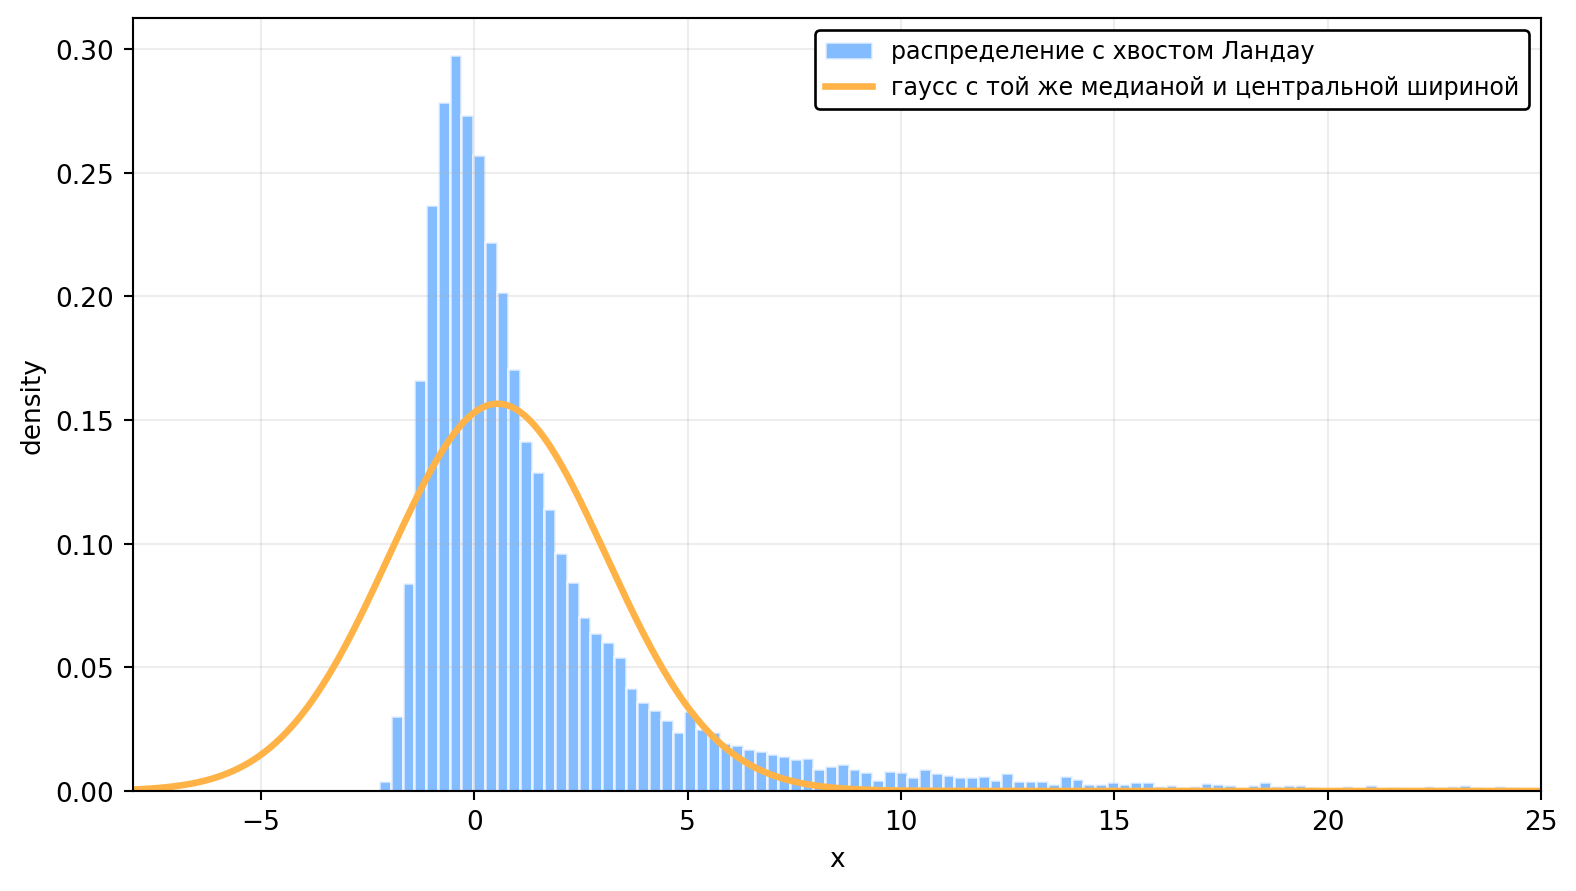
\includegraphics[keepaspectratio,alt={Ландау-подобное распределение с длинным правым хвостом и гауссовская кривая, построенная по той же медиане и центральной ширине.}]{chapters/../assets/figures/landau_like_default.png}}

\end{center}

\BookInlineFigureCaption{Ландау-подобное распределение с длинным правым хвостом и гауссовская
кривая, построенная по той же медиане и центральной ширине.}

\end{bookfigurepanel}

\subsection{Физические примеры и границы
приближения}\label{ux444ux438ux437ux438ux447ux435ux441ux43aux438ux435-ux43fux440ux438ux43cux435ux440ux44b-ux438-ux433ux440ux430ux43dux438ux446ux44b-ux43fux440ux438ux431ux43bux438ux436ux435ux43dux438ux44f}

\begin{itemize}
\item
  \(dE/dx\) в тонких кремниевых сенсорах;
\item
  Потери энергии в газовых трековых сенсорах;
\item
  ТРС: усечённое среднее используют именно для подавления длинного
  хвоста;
\item
  Калориметрические флуктуации с редкими большими локальными потерями.
\end{itemize}

\begin{booknote}

Распределение Ландау -- приближённая асимптотическая модель для тонкого
слоя вещества, где полная потеря энергии складывается из многих
независимых кулоновских столкновений, а спектр одиночных передач имеет
длинный хвост \(\propto1/\varepsilon^2\). Именно этот хвост делает
распределение полной потери энергии асимметричным и негауссовым.

В реальном веществе хвост ограничен кинематикой и атомной структурой.
При более точном описании возникает распределение Вавилова, которое в
пределе большой толщины переходит к распределению Гаусса.

\end{booknote}

\section{Коррелированные
слагаемые}\label{ux43aux43eux440ux440ux435ux43bux438ux440ux43eux432ux430ux43dux43dux44bux435-ux441ux43bux430ux433ux430ux435ux43cux44bux435}

Независимость случайных величин -- не формальное украшение центральной
предельной теоремы. Для суммы \[S_n=\sum_{i=1}^{n}X_i\] дисперсия
содержит ковариационные члены: \[\mathrm{Var}(S_n)
=
\sum_i\sigma_i^2
+2\sum_{i<j}\mathrm{cov}(X_i,X_j).\] Если слагаемые независимы,
ковариации равны нулю. При наличии корреляций дисперсия может
масштабироваться с ростом \(n\) совершенно иначе.

\subsection{Усреднение одинаково коррелированных
величин}\label{ux443ux441ux440ux435ux434ux43dux435ux43dux438ux435-ux43eux434ux438ux43dux430ux43aux43eux432ux43e-ux43aux43eux440ux440ux435ux43bux438ux440ux43eux432ux430ux43dux43dux44bux445-ux432ux435ux43bux438ux447ux438ux43d}

Пусть \[\mathrm{Var}(X_i)=\sigma^2,
\qquad
\mathrm{corr}(X_i,X_j)=\rho,
\qquad i\ne j.\] Выведем дисперсию для среднего:
\[\overline X=\frac1n\sum_{i=1}^{n}X_i.\]

\begin{bookderivation}

\subsubsection{\texorpdfstring{Дисперсия среднего при общей корреляции
\(\rho\)}{Дисперсия среднего при общей корреляции \textbackslash rho}}\label{ux434ux438ux441ux43fux435ux440ux441ux438ux44f-ux441ux440ux435ux434ux43dux435ux433ux43e-ux43fux440ux438-ux43eux431ux449ux435ux439-ux43aux43eux440ux440ux435ux43bux44fux446ux438ux438-rho}

Согласно общей формуле: \[\mathrm{Var}(\overline X)
=
\frac{1}{n^2}
\left(
\sum_i\sigma^2
+2\sum_{i<j}\mathrm{cov}(X_i,X_j)
\right).\] Если коэффициент корреляции для любой пары равен \(\rho\), то
\[\mathrm{cov}(X_i,X_j)=\rho\sigma^2.\] Число пар с \(i<j\) равно:
\[\frac{n(n-1)}{2}.\] Тогда
\[\mathrm{Var}(\overline X)=\frac{1}{n^2}\left[ n\sigma^2+2\frac{n(n-1)}{2}\rho\sigma^2\right]=
\frac{\sigma^2}{n}
\left[1+(n-1)\rho\right].\] При \(\rho=0\) остаётся привычное
\(\sigma^2/n\). Если \(\rho\ne0\), то \[\boxed{
\mathrm{Var}(\overline X)
\xrightarrow[n\to\infty]{}
\rho\sigma^2.
}\quad\blacksquare\]

\end{bookderivation}

Коррелированная часть не исчезает даже при бесконечном увеличении числа
измерений.

\section{Общий сдвиг как систематическая
ошибка}\label{ux43eux431ux449ux438ux439-ux441ux434ux432ux438ux433-ux43aux430ux43a-ux441ux438ux441ux442ux435ux43cux430ux442ux438ux447ux435ux441ux43aux430ux44f-ux43eux448ux438ux431ux43aux430}

Рассмотрим случайную величину: \[X_i=\mu+C+\epsilon_i,\] где общая для
всех измерений величина \(C\) и независимые статистические флуктуации
\(\epsilon_i\) имеют распределения: \[C\sim\mathrm{N}(0,\sigma_C^2),
\qquad
\epsilon_i\sim\mathrm{N}(0,\sigma_\epsilon^2).\] Среднее значение
\(X_i\) по \(n\) измерениям равно: \[\overline X
=
\mu+C+\frac1n\sum_i\epsilon_i.\]

\begin{bookderivation}

\subsubsection{Дисперсия среднего при общей систематической
составляющей}\label{ux434ux438ux441ux43fux435ux440ux441ux438ux44f-ux441ux440ux435ux434ux43dux435ux433ux43e-ux43fux440ux438-ux43eux431ux449ux435ux439-ux441ux438ux441ux442ux435ux43cux430ux442ux438ux447ux435ux441ux43aux43eux439-ux441ux43eux441ux442ux430ux432ux43bux44fux44eux449ux435ux439}

Общий сдвиг \(C\) присутствует одинаково во всех измерениях и при
усреднении не уменьшается. Независимая часть усредняется обычным
образом: \[\mathrm{Var}\!\left(\frac1n\sum_i\epsilon_i\right)
=
\frac{\sigma_\epsilon^2}{n}.\] Так как \(C\) и статистическая часть
независимы, получим \[\boxed{
\mathrm{Var}(\overline X)
=
\sigma_C^2
+
\frac{\sigma_\epsilon^2}{n}.
}\quad\blacksquare\]

\end{bookderivation}

При \(n\to\infty\) статистический член исчезает, но \(\sigma_C^2\)
остаётся.\textbackslash{} С физической точки зрения таким общим сдвигом
могут быть:

\begin{itemize}
\tightlist
\item
  ошибка энергетической шкалы детектора;
\item
  общая ошибка калибровки усиления;
\item
  неопределённость световыхода или коэффициента пересчёта АЦП в энергию;
\item
  общая ошибка нормировки потока, светимости или активности источника;
\item
  дрейф температуры, давления, высокого напряжения или усиления во время
  набора данных;
\item
  неопределённость нормировки общего фона;
\item
  общий временной сдвиг в измерениях времени пролёта.
\end{itemize}

Во всех этих случаях увеличение статистики уменьшает только независимую
часть ошибки. Общая систематическая составляющая при усреднении не
исчезает.

\begin{bookfigurepanel}

\begin{center}

\pandocbounded{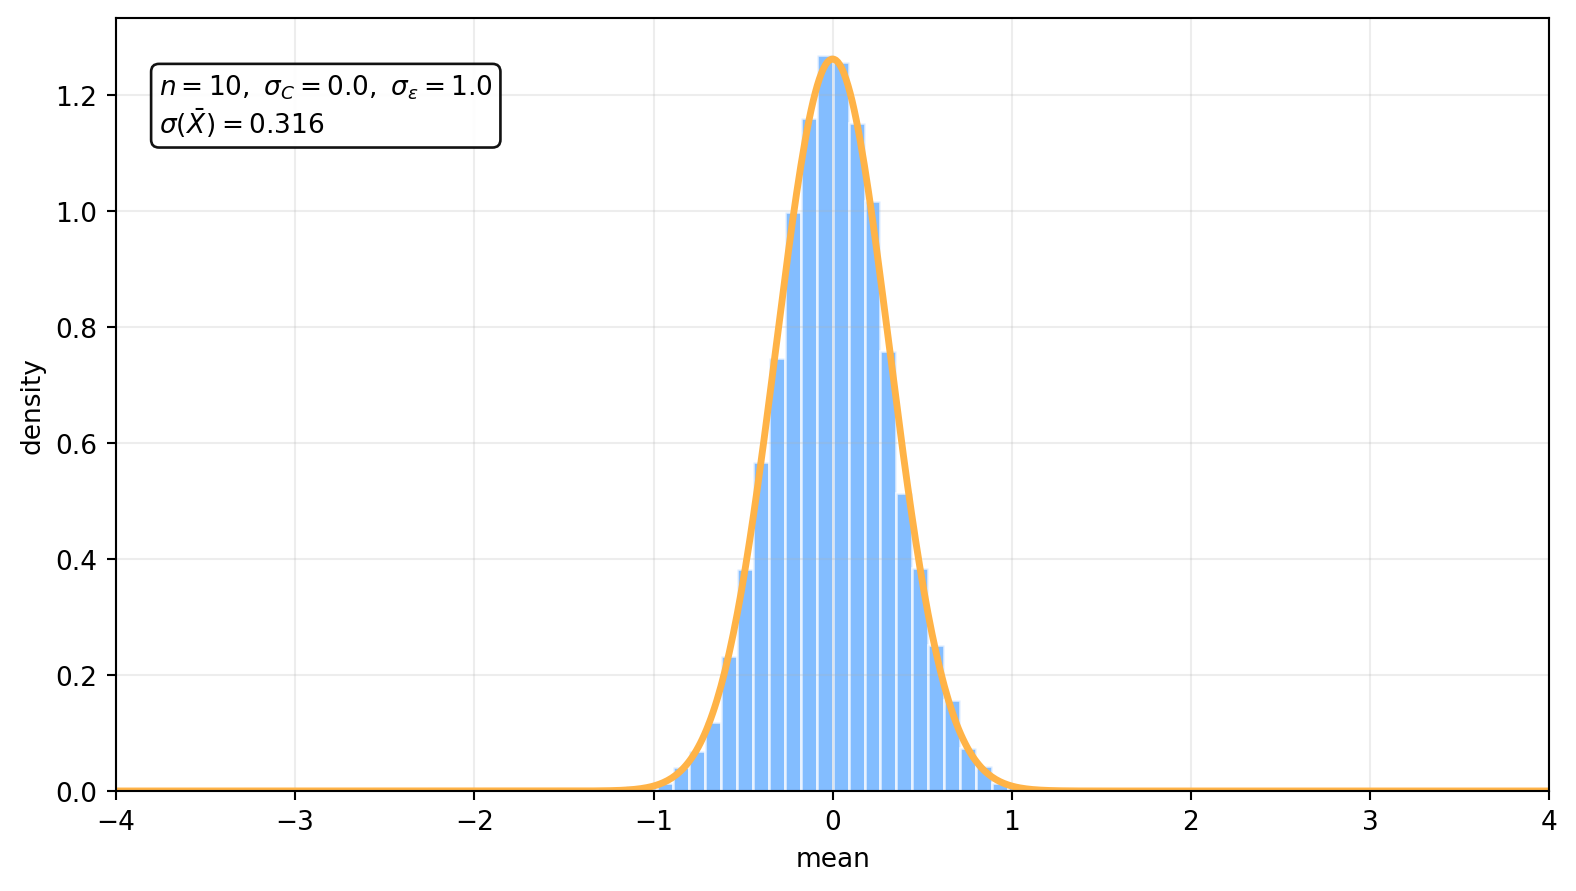
\includegraphics[keepaspectratio,alt={При отсутствии общей ошибки, \textbackslash sigma\_C=0, ширина среднего при n=100 определяется только статистической частью и заметно уменьшается.}]{chapters/../assets/figures/correlated_error_sigma0.png}}

\end{center}

\BookInlineFigureCaption{При отсутствии общей ошибки, \(\sigma_C=0\), ширина среднего при
\(n=100\) определяется только статистической частью и заметно
уменьшается.}

\end{bookfigurepanel}

\begin{bookfigurepanel}

\begin{center}

\pandocbounded{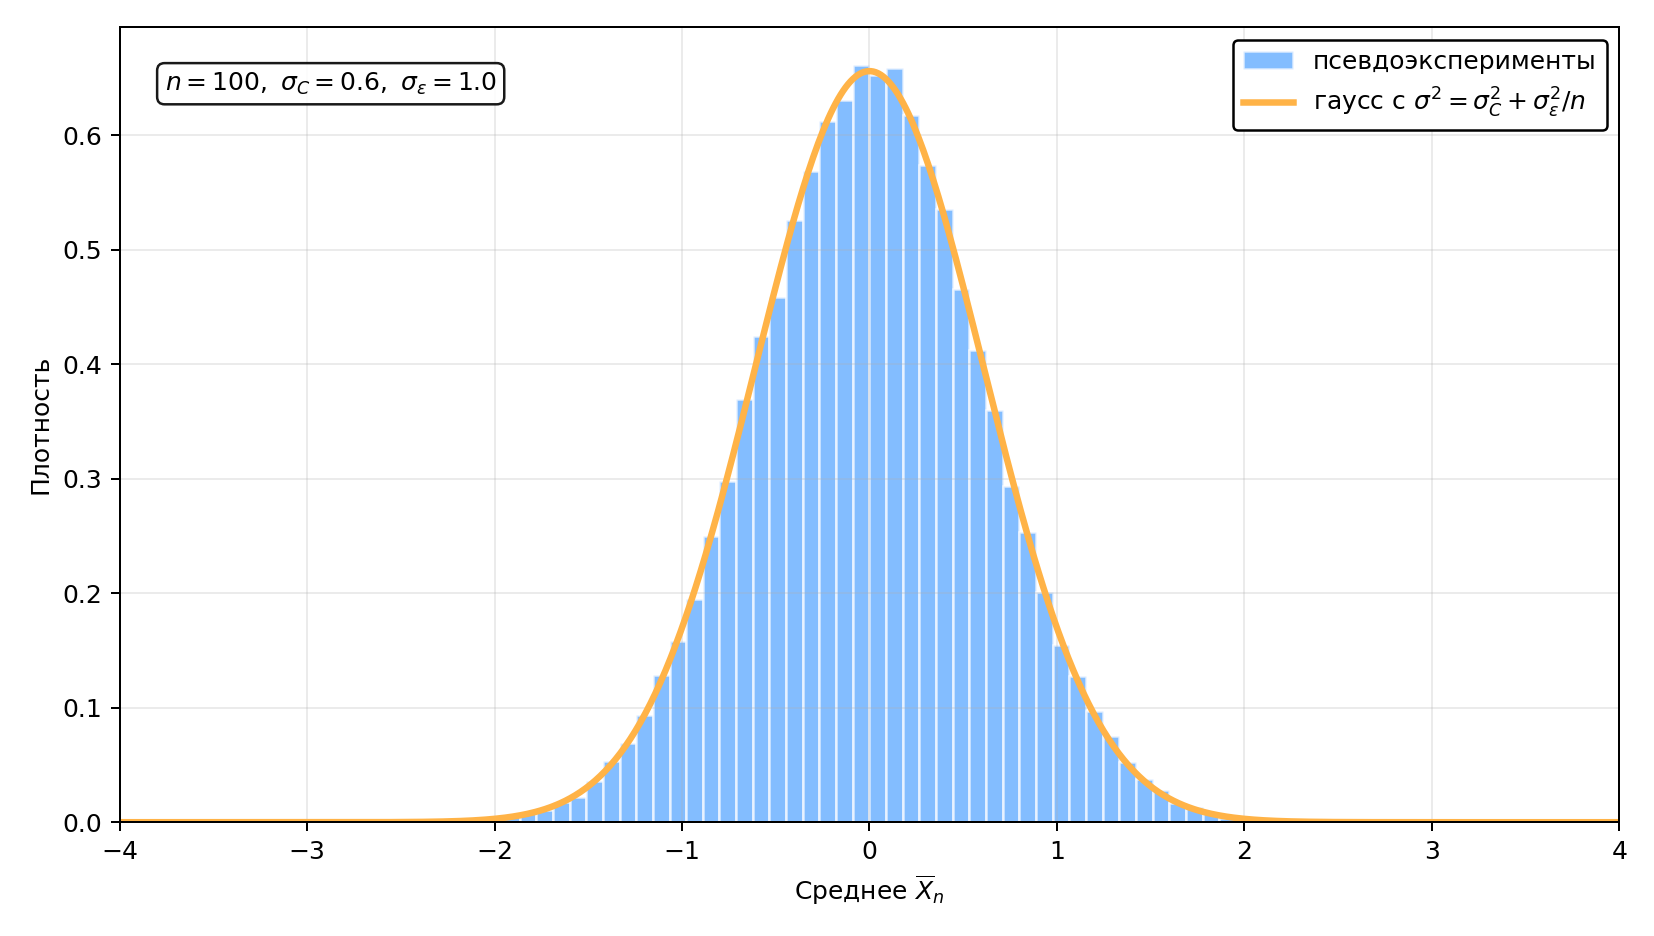
\includegraphics[keepaspectratio,alt={При той же статистике, но \textbackslash sigma\_C=0.6, общая составляющая доминирует в ширине распределения среднего и не исчезает при усреднении.}]{chapters/../assets/figures/correlated_error_sigma06.png}}

\end{center}

\BookInlineFigureCaption{При той же статистике, но \(\sigma_C=0.6\), общая составляющая
доминирует в ширине распределения среднего и не исчезает при усреднении.}

\end{bookfigurepanel}

Обратите внимание: итоговая форма при этом вполне может оставаться
визуально гауссовой. Проблема состоит не обязательно в форме
распределения, а в том, что его ширина содержит компоненту, не
уменьшающуюся с ростом статистики.

\section{Смеси
распределений}\label{ux441ux43cux435ux441ux438-ux440ux430ux441ux43fux440ux435ux434ux435ux43bux435ux43dux438ux439}

\subsection{Сумма и смесь -- разные
операции}\label{ux441ux443ux43cux43cux430-ux438-ux441ux43cux435ux441ux44c-ux440ux430ux437ux43dux44bux435-ux43eux43fux435ux440ux430ux446ux438ux438}

Пусть имеются две независимые пуассоновские величины:
\[N_1\sim\mathrm{Pois}(1000),
\qquad
N_2\sim\mathrm{Pois}(100).\] Если в каждом событии наблюдаются оба
вклада и они складываются, \[N=N_1+N_2,\] то для их суммы будет
справедливо: \[\boxed{N\sim\mathrm{Pois}(1100).}\] Смесь устроена иначе:
каждое отдельное событие принадлежит только одному из нескольких
классов. Сумма описывает сложение вкладов внутри события, а смесь --
объединение различных типов событий в одной выборке.

\subsection{Скрытый класс
события}\label{ux441ux43aux440ux44bux442ux44bux439-ux43aux43bux430ux441ux441-ux441ux43eux431ux44bux442ux438ux44f}

Пусть существует скрытая переменная \(\theta\), выбирающая механизм:
\[\theta=
\begin{cases}
1, & \text{первый класс},\\
2, & \text{второй класс}.
\end{cases}\] Условно на класс распределения могут быть:
\[N\mid\theta=1\sim\mathrm{Pois}(1000),
\qquad
N\mid\theta=2\sim\mathrm{Pois}(100).\] Наблюдатель видит только \(N\),
но не знает \(\theta\). Внутри каждого класса распределение может быть
узким, тогда как объединённая выборка оказывается широкой или даже
многопиковой.

\subsection{Условный гаусс не означает безусловный
гаусс}\label{ux443ux441ux43bux43eux432ux43dux44bux439-ux433ux430ux443ux441ux441-ux43dux435-ux43eux437ux43dux430ux447ux430ux435ux442-ux431ux435ux437ux443ux441ux43bux43eux432ux43dux44bux439-ux433ux430ux443ux441ux441}

Пусть при фиксированном скрытом параметре \(\theta\) \[X\mid\theta
\sim
\mathrm{N}(\mu_\theta,\sigma_\theta^2),\] Тогда, если \(\theta\) не
наблюдается, то полная плотность равна: \[p(x)
=
\int p(\theta)\,
\mathrm{N}(x;\mu_\theta,\sigma_\theta^2)\,d\theta.\] Это смесь
распределений Гаусса, которая в общем случае не обязана быть одним
гауссом.

\begin{booknote}

Полная дисперсия смеси состоит из двух частей: \[\boxed{
\mathrm{Var}(X)
=
\mathbb{E}_\theta\!\left[\mathrm{Var}(X\mid\theta)\right]
+
\mathrm{Var}_\theta\!\left(\mathbb{E}[X\mid\theta]\right).
}\] Для условных гауссовых распределений: \[\boxed{
\mathrm{Var}(X)
=
\mathbb{E}_\theta[\sigma_\theta^2]
+
\mathrm{Var}_\theta(\mu_\theta).
}\] Первое слагаемое -- средняя ширина распределений внутри классов.
Второе -- разброс средних между классами.

\end{booknote}

\subsection{Численный пример: два пуассоновских
класса}\label{ux447ux438ux441ux43bux435ux43dux43dux44bux439-ux43fux440ux438ux43cux435ux440-ux434ux432ux430-ux43fux443ux430ux441ux441ux43eux43dux43eux432ux441ux43aux438ux445-ux43aux43bux430ux441ux441ux430}

Пусть два класса равновероятны: \[N\mid\theta=1\sim\mathrm{Pois}(1000),
\qquad
N\mid\theta=2\sim\mathrm{Pois}(100).\] Средняя внутриклассовая дисперсия
равна: \[\mathbb{E}_\theta[\mathrm{Var}(N\mid\theta)]
=
\frac{1000+100}{2}
=550.\] Разброс средних классов:
\[\mathrm{Var}_\theta(\mathbb{E}[N\mid\theta])
=
\frac{(1000-550)^2+(100-550)^2}{2}
=202500.\] Полная дисперсия оказывается:
\[\boxed{\mathrm{Var}(N)=550+202500=203050.}\] Большая итоговая ширина в
этом примере возникает не из-за больших флуктуаций каждого отдельного
класса, а из-за того, что два класса имеют очень разные средние (скрытая
неоднородность выборки).

\begin{bookfigurepanel}

\begin{center}

\pandocbounded{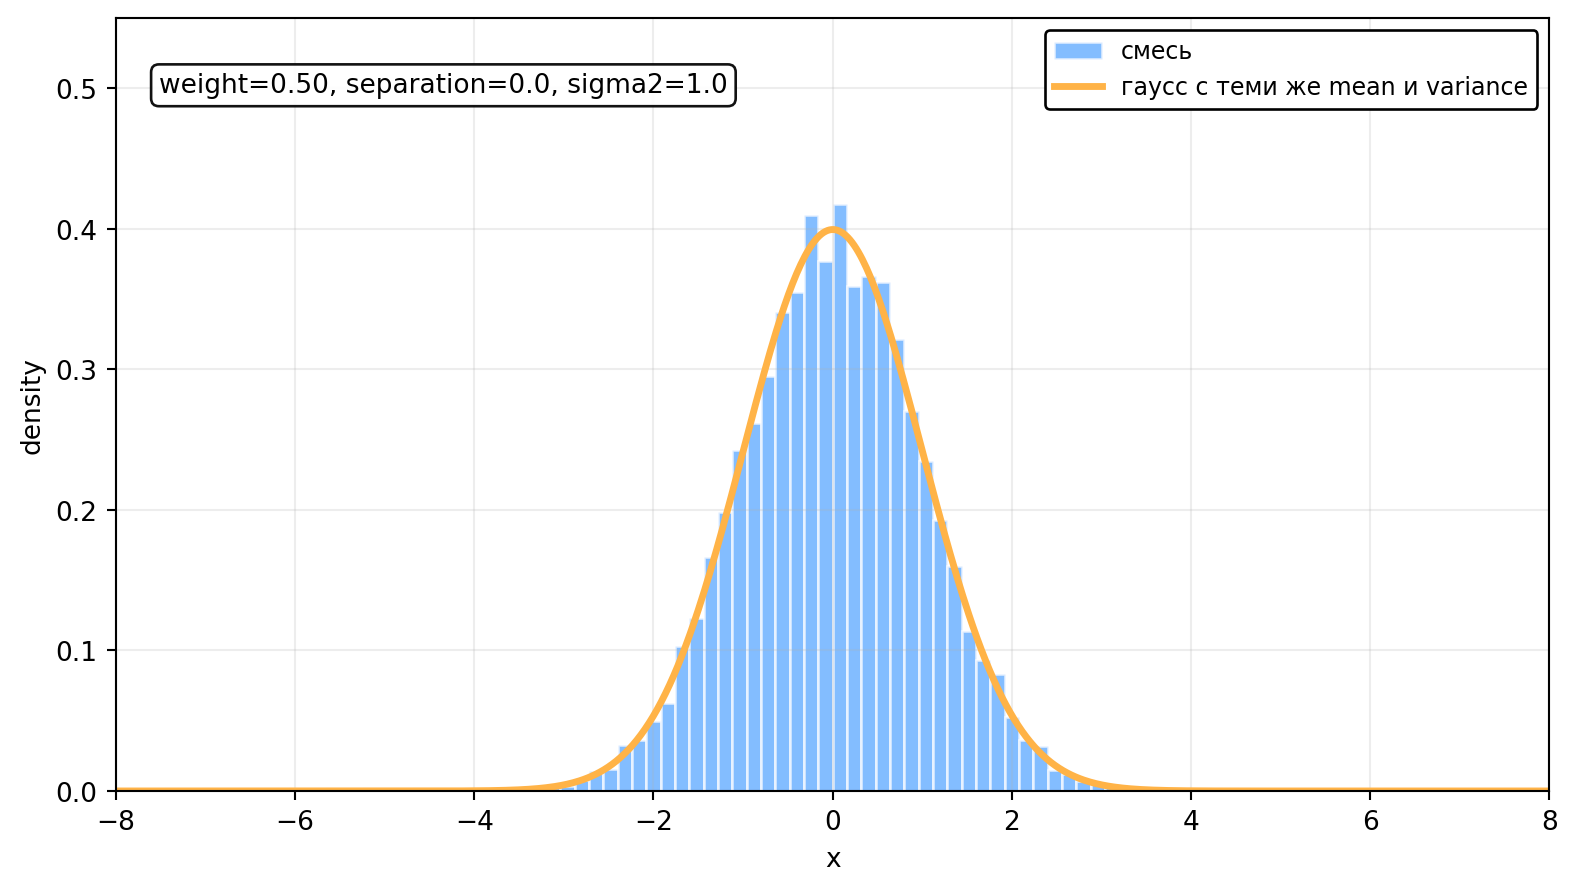
\includegraphics[keepaspectratio,alt={При нулевом расстоянии между средними смесь двух одинаковых гауссов визуально совпадает с одним гауссом.}]{chapters/../assets/figures/gaussian_mixture_sep0.png}}

\end{center}

\BookInlineFigureCaption{При нулевом расстоянии между средними смесь двух одинаковых гауссов
визуально совпадает с одним гауссом.}

\end{bookfigurepanel}

\begin{bookfigurepanel}

\begin{center}

\pandocbounded{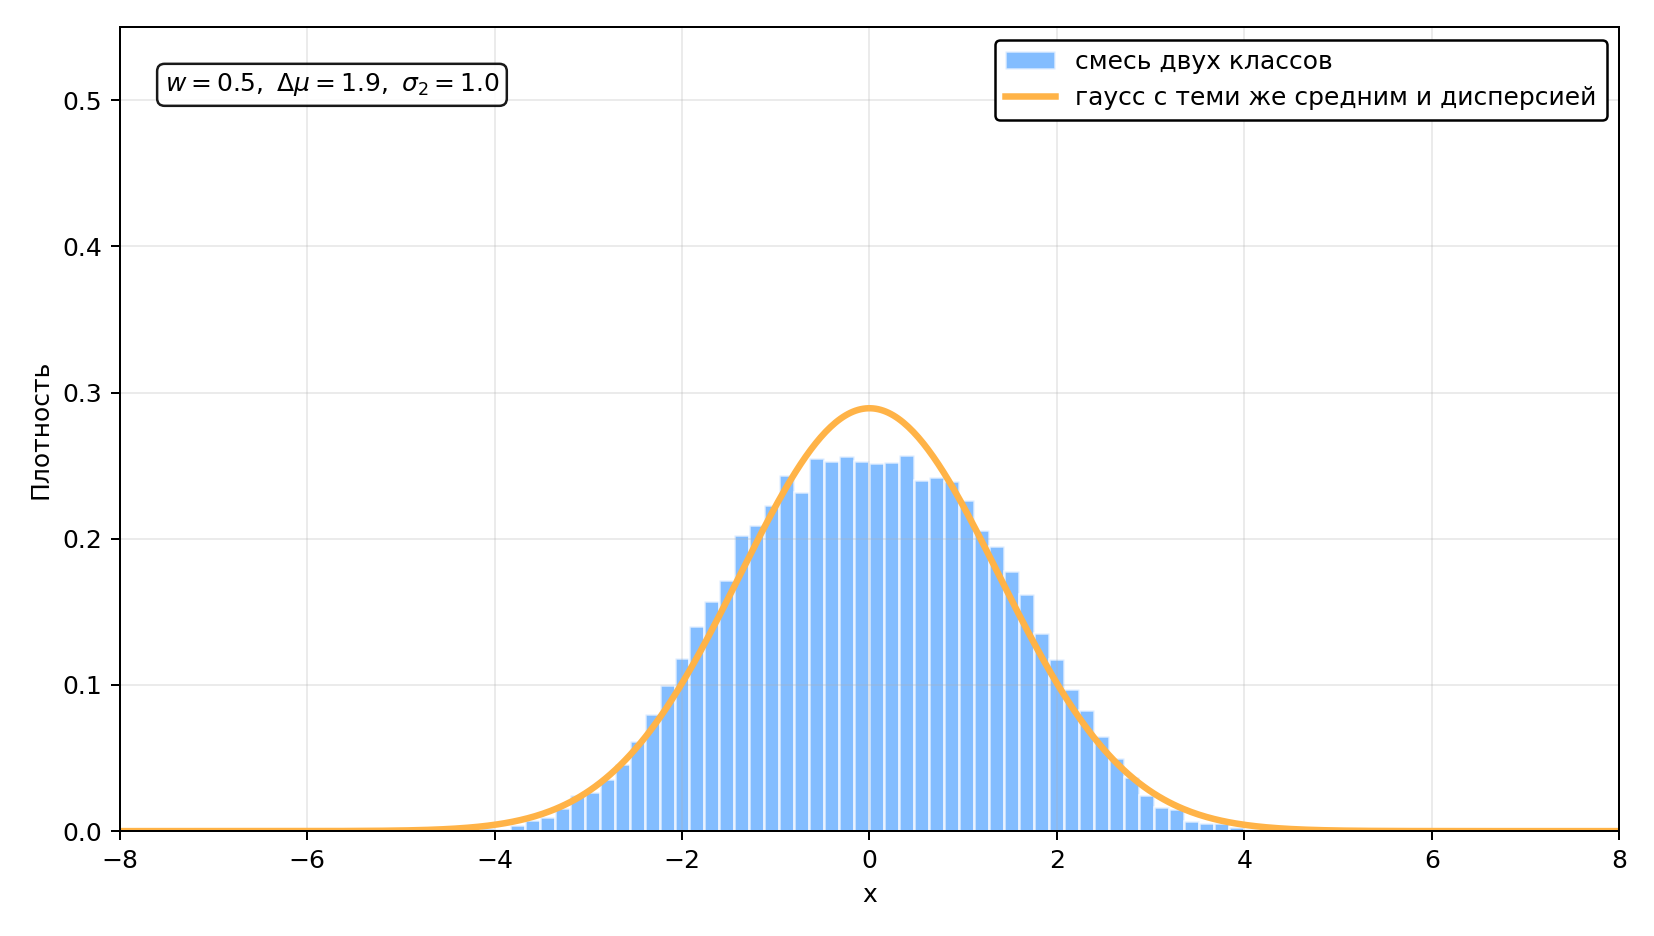
\includegraphics[keepaspectratio,alt={При умеренном разделении двух классов смесь всё ещё может выглядеть почти однопиковой, но её ширина уже содержит вклад разброса средних классов.}]{chapters/../assets/figures/gaussian_mixture_sep1_9.png}}

\end{center}

\BookInlineFigureCaption{При умеренном разделении двух классов смесь всё ещё может выглядеть
почти однопиковой, но её ширина уже содержит вклад разброса средних
классов.}

\end{bookfigurepanel}

\begin{bookfigurepanel}

\begin{center}

\pandocbounded{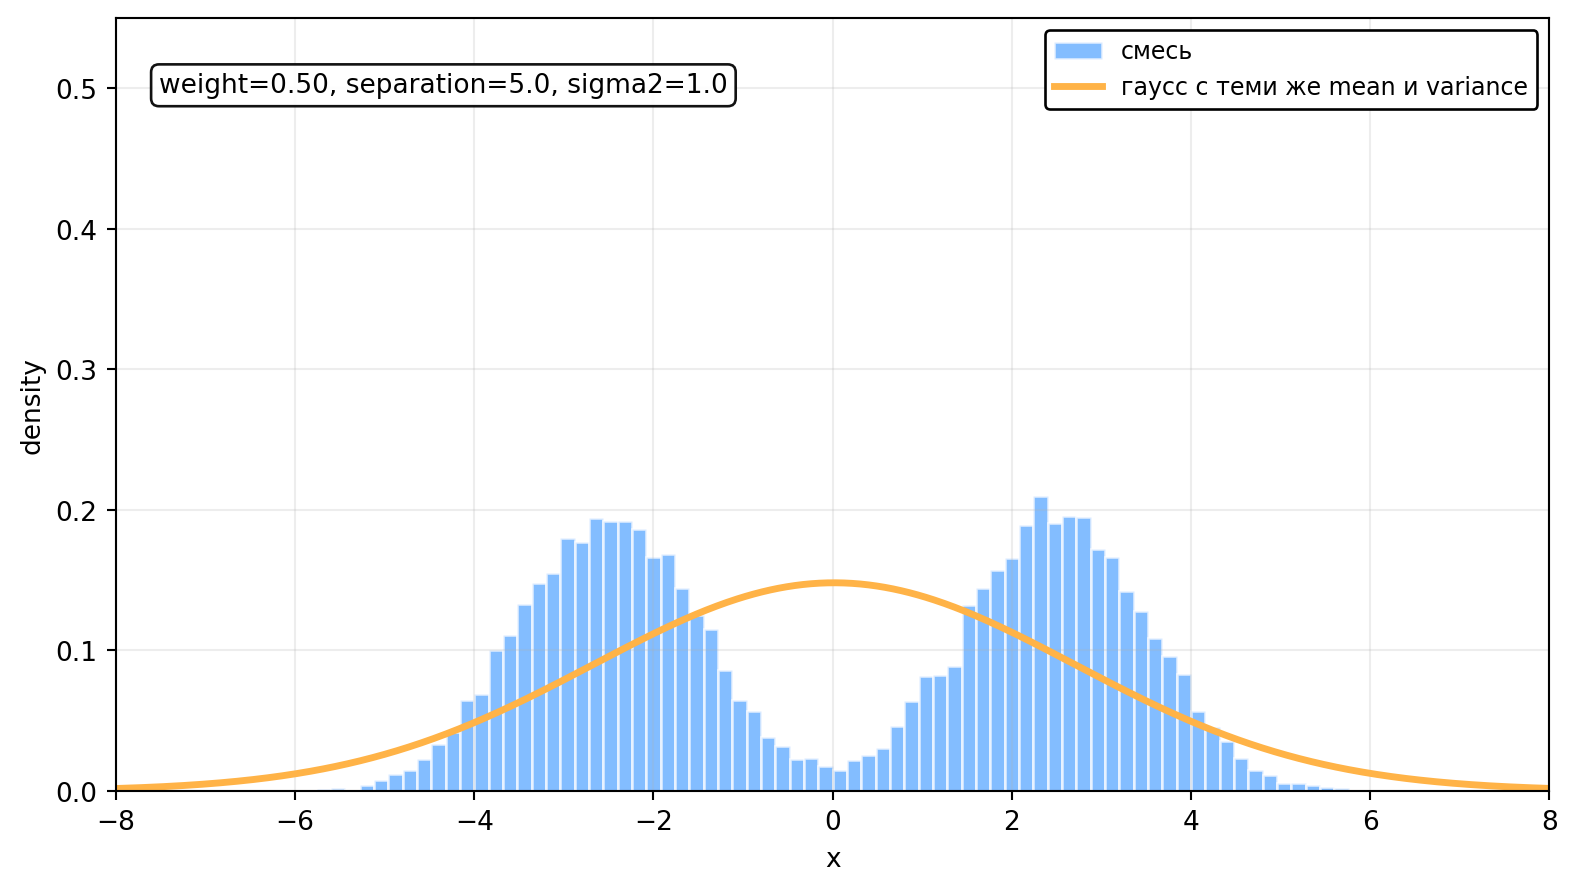
\includegraphics[keepaspectratio,alt={При большом расстоянии между средними скрытая двухклассовая структура становится явно двухпиковой.}]{chapters/../assets/figures/gaussian_mixture_sep5.png}}

\end{center}

\BookInlineFigureCaption{При большом расстоянии между средними скрытая двухклассовая структура
становится явно двухпиковой.}

\end{bookfigurepanel}

Даже если каждый класс сам по себе узок и хорошо описывается нормальным
распределением, их смесь может быть широкой, асимметричной или
многопиковой.

\section{Пример: жидкий
сцинтиллятор}\label{ux43fux440ux438ux43cux435ux440-ux436ux438ux434ux43aux438ux439-ux441ux446ux438ux43dux442ux438ux43bux43bux44fux442ux43eux440}

В жидком сцинтилляторе измеряемую величину можно схематично представить
как: \[Q
=
Q(E,\theta)
+
\text{фотонная статистика}
+
\text{электроника},\] где \(\theta\) описывает скрытые детали события: к
примеру, тип частицы, топологию, позицию, вклад от Черенковского
излучения, гашение или оптический путь. Например, для \(\gamma\)-кванта
энергия сначала передаётся вторичным электронам:
\[\gamma\to e_1+e_2+\cdots+e_m,\] причём \[E_\gamma=\sum_{a=1}^{m}E_a.\]
Полная энергия может быть одинаковой в разных событиях, но световой
выход нелинеен. Если \(L(E)\) -- световой отклик на электрон с энергией
\(E\), то \[Q\simeq\sum_a L(E_a),\] и в общем случае: \[\boxed{
Q\ne C\sum_aE_a.
}\] Таким образом, наблюдаемый отклик зависит не только от полной
энергии \(E_\gamma\), но и от того, как эта энергия распределилась между
вторичными частицами. Разные скрытые механизмы могут создавать
дополнительный вклад в энергетическое разрешение.

\section{Нелинейные преобразования: отношение случайных
величин}\label{ux43dux435ux43bux438ux43dux435ux439ux43dux44bux435-ux43fux440ux435ux43eux431ux440ux430ux437ux43eux432ux430ux43dux438ux44f-ux43eux442ux43dux43eux448ux435ux43dux438ux435-ux441ux43bux443ux447ux430ux439ux43dux44bux445-ux432ux435ux43bux438ux447ux438ux43d}

Гауссова форма исходных величин не гарантирует гауссову форму
произвольной функции от них. Пусть две независимые величины имеют
стандартные нормальные распределения: \[X,Y\sim\mathrm{N}(0,1).\]
Рассмотрим их отношение: \[R=\frac{X}{Y}.\] Оказывается, оно имеет
стандартное распределение Коши:

\begin{booknote}

\[\boxed{
f_R(r)=\frac{1}{\pi(1+r^2)}.}\] То есть отношение двух независимых
стандартных гауссовых величин уже не является гауссовой величиной.

\end{booknote}

Такие отношения возникают при нормировке на контрольную область, в
отношении двух скоростей счёта, в поправках на эффективность,
асимметриях вида: \[\frac{N_1-N_2}{N_1+N_2},\] а также при
восстановлении величины через деление на малую или шумную оценку.

\begin{bookfigurepanel}

\begin{center}

\pandocbounded{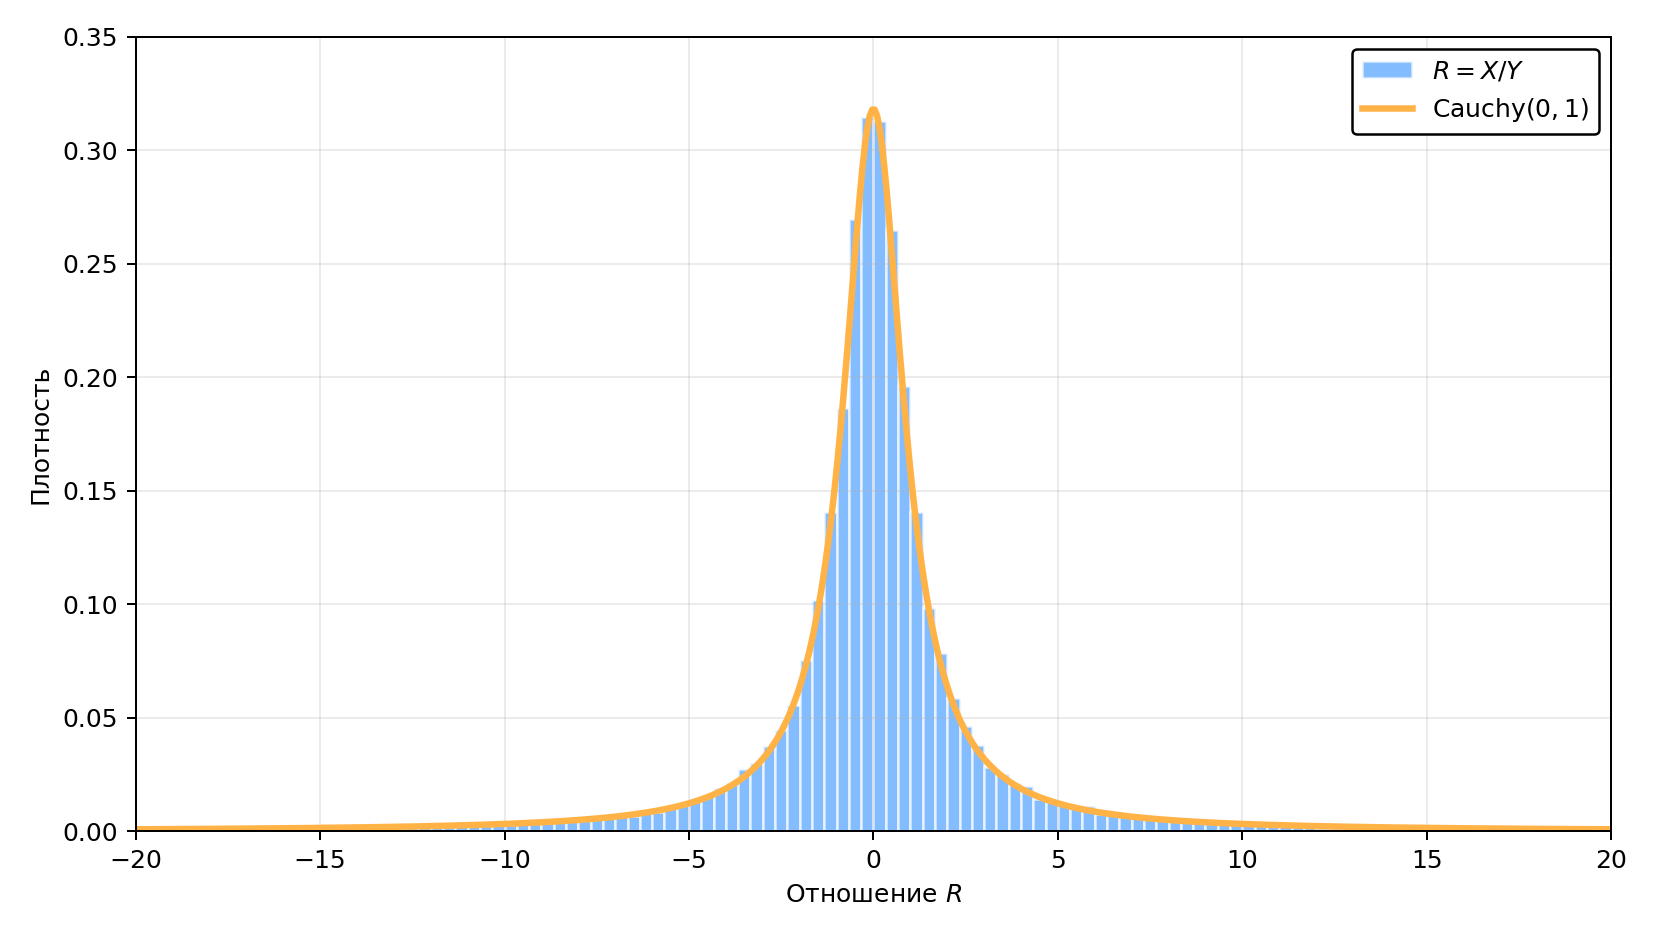
\includegraphics[keepaspectratio,alt={Отношение двух независимых стандартных гауссовых величин воспроизводит распределение Коши.}]{chapters/../assets/figures/ratio_gaussians_cauchy.png}}

\end{center}

\BookInlineFigureCaption{Отношение двух независимых стандартных гауссовых величин воспроизводит
распределение Коши.}

\end{bookfigurepanel}

\section{Сводная карта
причин}\label{ux441ux432ux43eux434ux43dux430ux44f-ux43aux430ux440ux442ux430-ux43fux440ux438ux447ux438ux43d}

{\def\LTcaptype{none} % do not increment counter
\begin{longtable}[]{@{}
  >{\centering\arraybackslash}p{(\linewidth - 4\tabcolsep) * \real{0.2500}}
  >{\centering\arraybackslash}p{(\linewidth - 4\tabcolsep) * \real{0.3750}}
  >{\centering\arraybackslash}p{(\linewidth - 4\tabcolsep) * \real{0.3750}}@{}}
\toprule\noalign{}
\begin{minipage}[b]{\linewidth}\centering
Механизм
\end{minipage} & \begin{minipage}[b]{\linewidth}\centering
Что нарушено
\end{minipage} & \begin{minipage}[b]{\linewidth}\centering
Типичный симптом
\end{minipage} \\
\midrule\noalign{}
\endhead
\bottomrule\noalign{}
\endlastfoot
Коши & нет конечной дисперсии & среднее не стабилизируется \\
Тяжёлые хвосты & медленная асимптотика & редкие большие выбросы \\
Доминирующий вклад & нет малости отдельных вкладов & хвост задаётся
одним механизмом \\
Корреляции & нарушена независимость & ошибка не падает как
\(1/\sqrt n\) \\
Смесь классов & разные \(\mu_\theta\) и \(\sigma_\theta\) & асимметрия,
хвосты, несколько пиков \\
Нелинейность & рассматривается не сумма, а функция \(f(X)\) &
асимметрия, границы \\
\end{longtable}
}

\section{Практический
алгоритм}\label{ux43fux440ux430ux43aux442ux438ux447ux435ux441ux43aux438ux439-ux430ux43bux433ux43eux440ux438ux442ux43c}

Перед тем как автоматически использовать распределение Гаусса, полезно
последовательно проверить физический смысл наблюдаемой величины:

\begin{enumerate}
\def\labelenumi{\arabic{enumi}.}
\tightlist
\item
  Какая случайная величина на самом деле суммируется?
\item
  Действительно ли отдельные вклады независимы?
\item
  Конечна ли дисперсия и нет ли тяжёлых хвостов?
\item
  Не существует ли скрытых классов событий?
\item
  Не применено ли нелинейное преобразование случайных величин?
\end{enumerate}

Если после этих проверок гауссово приближение выглядит сомнительно, это
не означает, что анализ невозможен. Не нужно заранее навязывать данным
нормальную форму. Распределение можно получать моделированием, в
частности методом Монте-Карло, и использовать полученную форму при
построении функции правдоподобия.

\begin{bookchaptersummary}[Итоги главы]

\begin{itemize}
\tightlist
\item
  Центральная предельная теорема требует не просто большого числа
  слагаемых, а конкретных условий на их дисперсии, независимость и
  относительный размер вкладов.
\item
  Среднее независимых величин Коши не сужается при росте \(n\) и
  сохраняет распределение Коши.
\item
  Редкие большие энергетические потери создают длинный хвост
  распределения Ландау и нарушают обычный механизм гауссова предела.
\item
  Корреляции и общие систематические ошибки оставляют вклад в дисперсию,
  который не исчезает при увеличении статистики.
\item
  Смесь разных классов событий принципиально отличается от суммы
  случайных вкладов и может создавать дополнительную дисперсию или
  многопиковость.
\item
  Нелинейные преобразования способны радикально менять форму
  распределения: отношение двух стандартных гауссовых величин имеет
  распределение Коши.
\item
  Перед использованием приближения Гаусса нужно проверить физический
  механизм образования наблюдаемой величины, а при сомнениях опираться
  на моделирование распределения, а не на автоматическое предположение
  нормальности.
\end{itemize}

\end{bookchaptersummary}

\section{Материалы
курса}\label{ux43cux430ux442ux435ux440ux438ux430ux43bux44b-ux43aux443ux440ux441ux430-2}

\begin{itemize}
\tightlist
\item
  \href{https://neutrinohit.github.io/statistical-analysis-course/ru/slides/04_non_gaussian_clt_violations.html}{Слайды
  лекции}
\item
  \href{https://neutrinohit.github.io/statistical-analysis-course/ru/slides/exercises/04_non_gaussian_clt_violations_exercises.html}{Задачи}
\end{itemize}

\part{II. Моделирование и оценивание}

\chapter{Распространение ошибок, ковариации и многомерный
гаусс}\label{ux440ux430ux441ux43fux440ux43eux441ux442ux440ux430ux43dux435ux43dux438ux435-ux43eux448ux438ux431ux43eux43a-ux43aux43eux432ux430ux440ux438ux430ux446ux438ux438-ux438-ux43cux43dux43eux433ux43eux43cux435ux440ux43dux44bux439-ux433ux430ux443ux441ux441}

\begin{bookchapteropening}[Главная мысль]

Неопределённость производной физической величины определяется не только
ошибками исходных измерений, но и чувствительностью результата к каждому
из них и взаимными корреляциями между измерениями. При малых ошибках эту
зависимость можно линеаризовать, после чего распространение
неопределённостей сводится к работе с производными и ковариационной
матрицей. Та же матрица задаёт форму многомерного гауссовского
распределения: её диагональные элементы отвечают за масштабы флуктуаций,
внедиагональные --- за корреляции, а вероятностные области становятся
эллипсами и эллипсоидами.

\end{bookchapteropening}

\section{План
главы}\label{ux43fux43bux430ux43d-ux433ux43bux430ux432ux44b-4}

\begin{itemize}
\tightlist
\item
  От непосредственно измеряемых величин к физическому результату
\item
  Линейное распространение ошибки для одной переменной
\item
  Когда линейное приближение перестаёт работать
\item
  Разброс оценок среднего, дисперсии и стандартного отклонения
\item
  Ковариация и коэффициент корреляции
\item
  Распространение ошибок для нескольких переменных
\item
  Ковариационная матрица и матричная запись распространения
\item
  Двумерное нормальное распределение и расстояние Махаланобиса
\item
  Эллипсы и вероятностные контуры
\item
  Усреднение измерений и пример с инвариантной массой
\item
  Когда переходить от аналитической формулы к Монте-Карло
\end{itemize}

\section{От измерения к физическому
результату}\label{ux43eux442-ux438ux437ux43cux435ux440ux435ux43dux438ux44f-ux43a-ux444ux438ux437ux438ux447ux435ux441ux43aux43eux43cux443-ux440ux435ux437ux443ux43bux44cux442ux430ux442ux443}

Эксперимент обычно не измеряет непосредственно ту величину, которая
затем появляется в физическом результате. Детектор регистрирует набор
исходных величин

\[
\mathbf X=(X_1,\ldots,X_n),
\]

а интересующий результат строится как функция этих измерений:

\[
\mathbf Y=\mathbf f(\mathbf X).
\]

Вместе со значением \(\mathbf Y\) необходимо сообщить его
неопределённость. Если \(\mathbf Y\) зависит от нескольких исходных
измерений, знания только их отдельных ошибок недостаточно: нужно также
понимать, как эти величины флуктуируют совместно.

\begin{booknote}

Типичные производные величины в эксперименте:

\begin{itemize}
\tightlist
\item
  поперечный импульс заряженной частицы из радиуса кривизны трека,
  \[p_T=qBR;\]
\item
  сечение процесса по числу событий, эффективности и интегральной
  светимости, \[\sigma=\frac{N_{\mathrm{sig}}}{\varepsilon L};\]
\item
  инвариантная масса двух безмассовых частиц,
  \[m^2=2E_1E_2(1-\cos\theta);\]
\item
  координаты точки пересечения восстановленных треков.
\end{itemize}

Во всех этих случаях неопределённости исходных измерений нужно перенести
на итоговый результат.

\end{booknote}

Основная идея состоит в локальной линеаризации. Если ошибки достаточно
малы, функцию можно заменить касательной в окрестности среднего
значения:

\[
\boxed{
f(X)\approx f(\mu_X)+f'(\mu_X)(X-\mu_X).
}
\]

Случайное отклонение \(X-\mu_X\) тогда преобразуется почти линейно, и
его дисперсию можно вычислить аналитически. Это приближение называется
\textbf{линейным распространением ошибок}.

\section{Одна измеряемая
величина}\label{ux43eux434ux43dux430-ux438ux437ux43cux435ux440ux44fux435ux43cux430ux44f-ux432ux435ux43bux438ux447ux438ux43dux430}

\subsection{Линейное распространение
ошибки}\label{ux43bux438ux43dux435ux439ux43dux43eux435-ux440ux430ux441ux43fux440ux43eux441ux442ux440ux430ux43dux435ux43dux438ux435-ux43eux448ux438ux431ux43aux438}

Пусть

\[
Y=f(X),
\qquad
\mathbb E[X]=\mu_X,
\qquad
\operatorname{Var}(X)=\sigma_X^2.
\]

Разложим функцию вблизи \(\mu_X\) и оставим только линейный член.

\begin{bookderivation}

\subsubsection{Вывод формулы для одной
переменной}\label{ux432ux44bux432ux43eux434-ux444ux43eux440ux43cux443ux43bux44b-ux434ux43bux44f-ux43eux434ux43dux43eux439-ux43fux435ux440ux435ux43cux435ux43dux43dux43eux439}

В первом порядке разложения Тейлора

\[
f(X)\approx f(\mu_X)+f'(\mu_X)(X-\mu_X).
\]

При таком приближении среднее значение результата равно

\[
\mathbb E[Y]\approx f(\mu_X),
\]

а отклонение от среднего имеет вид

\[
Y-\mathbb E[Y]
\approx
f'(\mu_X)(X-\mu_X).
\]

Возводя это выражение в квадрат и усредняя, получаем

\[
\begin{aligned}
\sigma_Y^2
&=\operatorname{Var}(Y)
\approx
\mathbb E\!\left[
\bigl(f'(\mu_X)(X-\mu_X)\bigr)^2
\right]\\
&=
\left[f'(\mu_X)\right]^2
\mathbb E[(X-\mu_X)^2].
\end{aligned}
\]

Следовательно,

\[
\boxed{
\sigma_Y^2
\approx
\left[f'(\mu_X)\right]^2\sigma_X^2,
\qquad
\sigma_Y
\approx
\left|f'(\mu_X)\right|\sigma_X.
}
\quad\blacksquare
\]

\end{bookderivation}

Формула показывает локальный смысл распространения ошибки: чем быстрее
меняется функция около измеренного значения, тем сильнее та же самая
исходная флуктуация \(X\) влияет на результат \(Y\).

\subsection{Пример: степенная
зависимость}\label{ux43fux440ux438ux43cux435ux440-ux441ux442ux435ux43fux435ux43dux43dux430ux44f-ux437ux430ux432ux438ux441ux438ux43cux43eux441ux442ux44c}

Для

\[Y=X^a\]

производная равна

\[
\frac{dY}{dX}=aX^{a-1}.
\]

Отсюда

\[
\sigma_Y\approx |a|\mu_X^{a-1}\sigma_X.
\]

Разделив обе части на \(|Y|=|\mu_X|^a\), получаем относительную форму:

\[
\boxed{
\frac{\sigma_Y}{|Y|}
\approx
|a|\frac{\sigma_X}{|\mu_X|}.
}
\]

Несколько часто используемых следствий этой формулы:

{\def\LTcaptype{none} % do not increment counter
\begin{longtable}[]{@{}ll@{}}
\toprule\noalign{}
Функция & Распространённая ошибка \\
\midrule\noalign{}
\endhead
\bottomrule\noalign{}
\endlastfoot
\(Y=aX+b\) & \(\sigma_Y=|a|\sigma_X\) \\
\(Y=X^a\) & \(\sigma_Y/|Y|\approx |a|\sigma_X/|X|\) \\
\(Y=1/X\) & \(\sigma_Y/|Y|\approx \sigma_X/|X|\) \\
\(Y=\ln X\) & \(\sigma_Y\approx \sigma_X/|X|\) \\
\(Y=e^X\) & \(\sigma_Y/|Y|\approx \sigma_X\) \\
\end{longtable}
}

\begin{booknote}

Эти формулы являются локальными. Производная не должна заметно
изменяться на масштабе исходной неопределённости. Если функция сильно
искривлена внутри области, где находится существенная часть
распределения \(X\), линейная формула может стать неточной.

\end{booknote}

\subsection{Пример: поперечный импульс в магнитном
поле}\label{ux43fux440ux438ux43cux435ux440-ux43fux43eux43fux435ux440ux435ux447ux43dux44bux439-ux438ux43cux43fux443ux43bux44cux441-ux432-ux43cux430ux433ux43dux438ux442ux43dux43eux43c-ux43fux43eux43bux435}

Пусть \(R\) --- измеренный радиус кривизны трека, а \(B\) --- магнитное
поле. Тогда

\[
p_T=qBR.
\]

Если \(B\) и \(q\) считаются известными, а неопределённость связана
только с измерением \(R\), то

\[
\frac{\partial p_T}{\partial R}=qB,
\]

и линейное распространение даёт

\[
\boxed{
\sigma_{p_T}=qB\sigma_R,
\qquad
\frac{\sigma_{p_T}}{p_T}=\frac{\sigma_R}{R}.
}
\]

\subsection{Пример: сечение
процесса}\label{ux43fux440ux438ux43cux435ux440-ux441ux435ux447ux435ux43dux438ux435-ux43fux440ux43eux446ux435ux441ux441ux430}

Рассмотрим

\[
\sigma=\frac{N}{\varepsilon L},
\]

где \(N\) --- число событий, \(\varepsilon\) --- эффективность, а \(L\)
--- интегральная светимость. Если ковариации между этими величинами
равны нулю, то результат для дисперсии имеет вид

\[
\sigma_\sigma^2
=
\frac{\sigma_N^2}{\varepsilon^2L^2}
+
\frac{N^2\sigma_\varepsilon^2}{\varepsilon^4L^2}
+
\frac{N^2\sigma_L^2}{\varepsilon^2L^4}.
\]

Удобнее переписать его в относительной форме:

\[
\boxed{
\left(\frac{\sigma_\sigma}{\sigma}\right)^2
=
\left(\frac{\sigma_N}{N}\right)^2
+
\left(\frac{\sigma_\varepsilon}{\varepsilon}\right)^2
+
\left(\frac{\sigma_L}{L}\right)^2.
}
\]

Обратите внимание: здесь специально предполагается нулевая ковариация.
Общая формула с корреляциями будет получена ниже.

\section{Когда линейное приближение работает
плохо}\label{ux43aux43eux433ux434ux430-ux43bux438ux43dux435ux439ux43dux43eux435-ux43fux440ux438ux431ux43bux438ux436ux435ux43dux438ux435-ux440ux430ux431ux43eux442ux430ux435ux442-ux43fux43bux43eux445ux43e}

Линейная формула основана на замене функции касательной. Из этого сразу
видно несколько ситуаций, где приближение становится ненадёжным:

\begin{itemize}
\tightlist
\item
  \(\sigma_X\) велика по сравнению с масштабом изменения \(f(X)\);
\item
  производная в точке разложения близка к нулю, и квадратичный член
  становится главным;
\item
  функция имеет порог, особенность или физическую границу;
\item
  после преобразования распределение становится заметно асимметричным.
\end{itemize}

Простейший пример --- \(Y=X^2\) при \(\mu_X=0\). Производная
\(dY/dX=2X\) в точке среднего равна нулю, поэтому линейная формула
формально даёт \(\sigma_Y\approx0\), хотя сама величина \(X^2\) очевидно
флуктуирует.

\subsection{\texorpdfstring{Нелинейное преобразование
\(Y=X+aX^2\)}{Нелинейное преобразование Y=X+aX\^{}2}}\label{ux43dux435ux43bux438ux43dux435ux439ux43dux43eux435-ux43fux440ux435ux43eux431ux440ux430ux437ux43eux432ux430ux43dux438ux435-yxax2}

Рассмотрим

\[
X\sim\mathrm N(1,\sigma_X^2),
\qquad
Y=X+aX^2.
\]

Линейное приближение около \(\mu_X=1\) предсказывает

\[
\boxed{
\mathbb E[Y]\approx1+a,
\qquad
\sigma_Y\approx |1+2a|\sigma_X.
}
\]

Для гауссовой \(X\) точные первые два момента равны

\[
\boxed{
\mathbb E[Y]=1+a+a\sigma_X^2,
\qquad
\sigma_Y^2=(1+2a)^2\sigma_X^2+2a^2\sigma_X^4.
}
\]

Отброшенные квадратичные члены создают одновременно смещение среднего и
дополнительную дисперсию.

\begin{bookfigurepanel}

\begin{center}

\pandocbounded{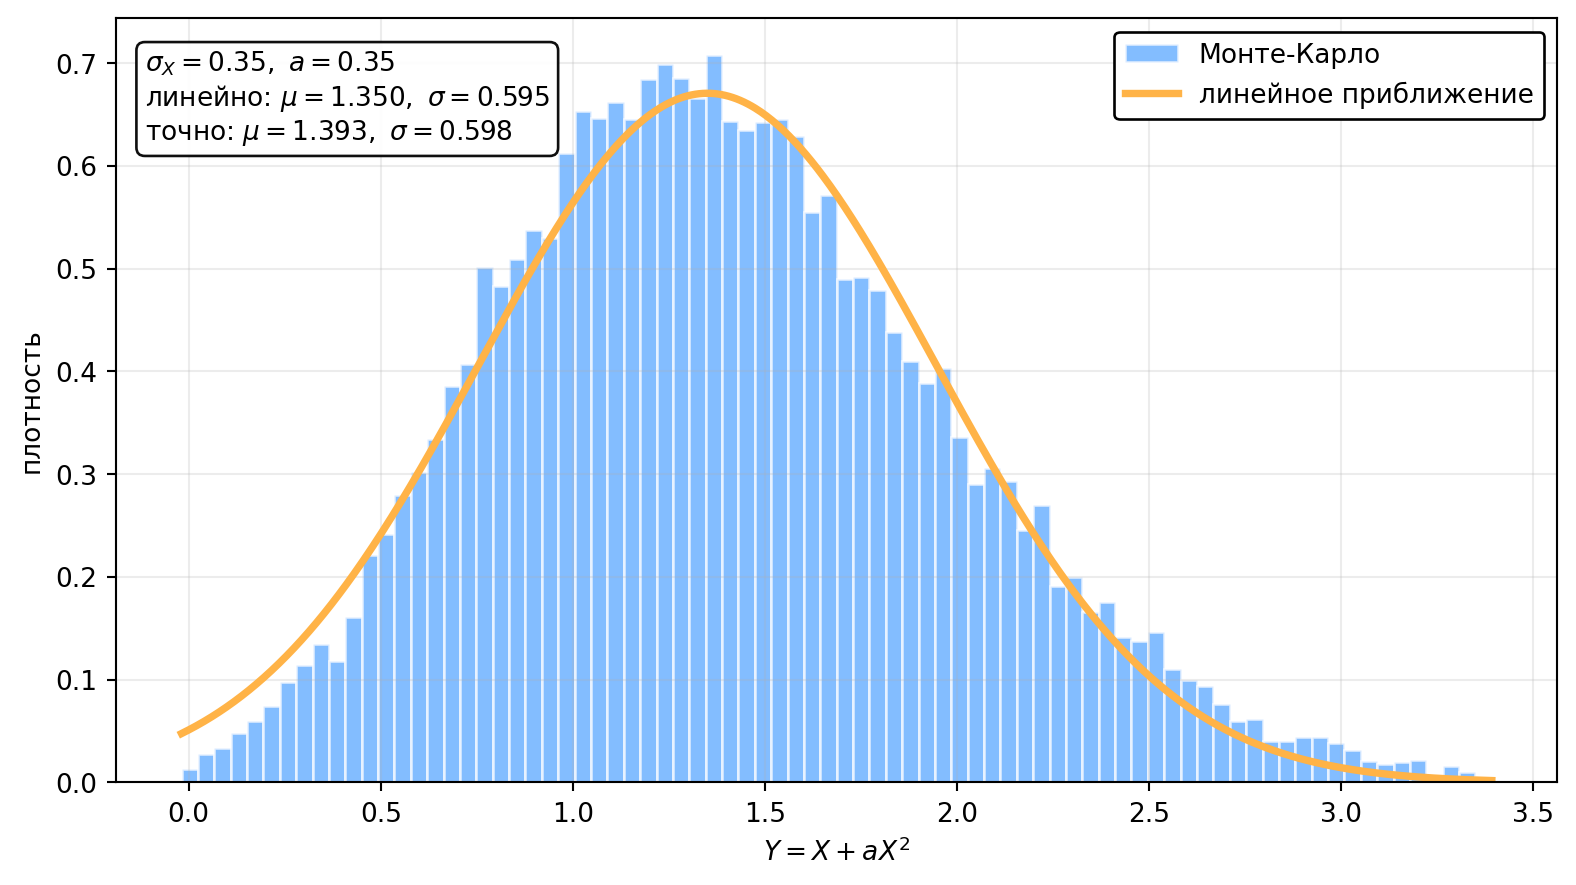
\includegraphics[keepaspectratio,alt={При \textbackslash sigma\_X=0.35 и a=0.35 линейное приближение ещё хорошо описывает центральную часть распределения, хотя точное среднее уже немного смещено.}]{chapters/../assets/figures/error_propagation_nonlinear_default.png}}

\end{center}

\BookInlineFigureCaption{При \(\sigma_X=0.35\) и \(a=0.35\) линейное приближение ещё хорошо
описывает центральную часть распределения, хотя точное среднее уже
немного смещено.}

\end{bookfigurepanel}

\begin{bookfigurepanel}

\begin{center}

\pandocbounded{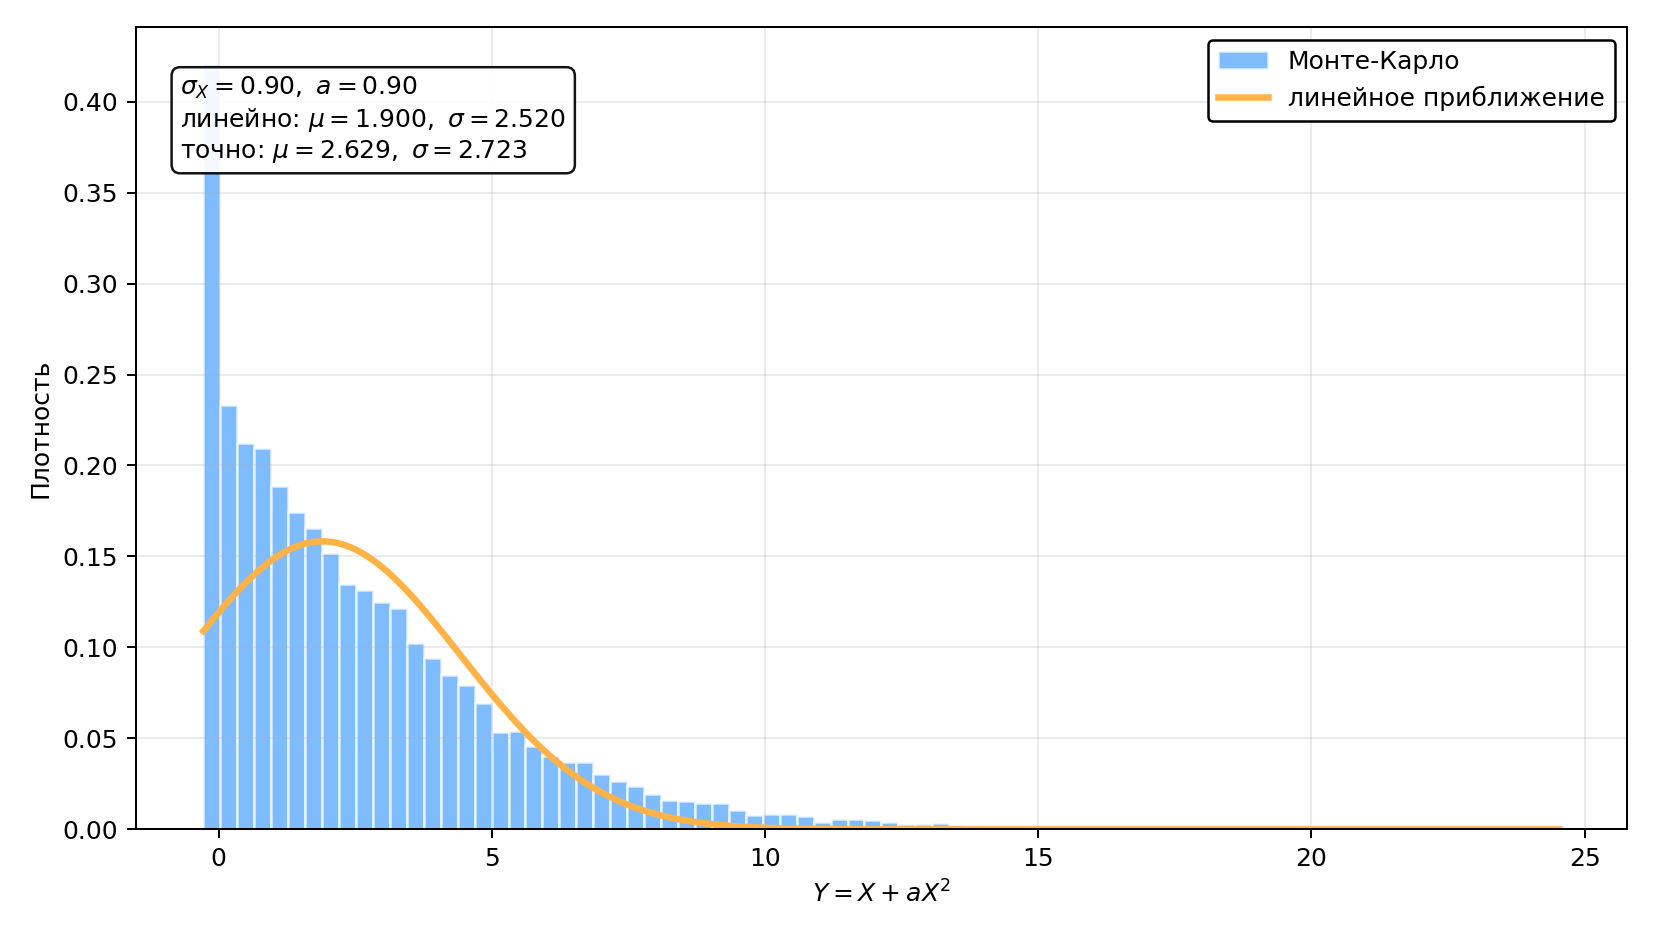
\includegraphics[keepaspectratio,alt={При больших \textbackslash sigma\_X и a нелинейность становится существенной: распределение Y заметно асимметрично, а линейный гауссовский прогноз уже не описывает его форму.}]{chapters/../assets/figures/error_propagation_nonlinear_strong.png}}

\end{center}

\BookInlineFigureCaption{При больших \(\sigma_X\) и \(a\) нелинейность становится существенной:
распределение \(Y\) заметно асимметрично, а линейный гауссовский прогноз
уже не описывает его форму.}

\end{bookfigurepanel}

При малых \(a\) и \(\sigma_X\) линейная формула и фактическое
распределение согласуются хорошо. При усилении нелинейности
распределение смещается и становится асимметричным, а одной симметричной
ошибки \(\sigma_Y\) уже недостаточно для точного описания.

\section{Разброс оценки стандартного
отклонения}\label{ux440ux430ux437ux431ux440ux43eux441-ux43eux446ux435ux43dux43aux438-ux441ux442ux430ux43dux434ux430ux440ux442ux43dux43eux433ux43e-ux43eux442ux43aux43bux43eux43dux435ux43dux438ux44f}

До сих пор \(\mu\) и \(\sigma\) рассматривались как параметры
распределения. В реальном эксперименте они обычно неизвестны и
оцениваются по конечной выборке. Пусть

\[
X_1,\ldots,X_N\sim\mathrm N(\mu,\sigma^2)
\]

--- независимые измерения одной и той же величины. По выборке строятся
оценки

\[
\widehat\mu
=
\frac1N\sum_{k=1}^{N}X_k,
\qquad
\widehat{\sigma^2}
=
\frac{1}{N-1}\sum_{k=1}^{N}(X_k-\widehat\mu)^2,
\]

и

\[
\widehat\sigma=\sqrt{\widehat{\sigma^2}}.
\]

\begin{booknote}

Величины \(\widehat\mu\), \(\widehat{\sigma^2}\) и \(\widehat\sigma\)
сами являются случайными. Если повторить весь эксперимент много раз, в
каждом повторении получится своё значение оценки. Значит, можно
обсуждать не только оценку дисперсии, но и \textbf{дисперсию самой
оценки}.

\end{booknote}

Для среднего при независимых гауссовых измерениях истинная дисперсия
равна

\[
\operatorname{Var}(\widehat\mu)=\frac{\sigma^2}{N}.
\]

Поскольку истинное \(\sigma^2\) обычно неизвестно, на практике
используют

\[
\widehat{\operatorname{Var}}(\widehat\mu)
=
\frac{\widehat{\sigma^2}}{N},
\qquad
\widehat\sigma_{\widehat\mu}
=
\frac{\widehat\sigma}{\sqrt N}.
\]

Но \(\widehat\sigma\) тоже найдено по конечной выборке. Теперь оценим,
насколько оно само флуктуирует.

\subsection{Несмещённость выборочной
дисперсии}\label{ux43dux435ux441ux43cux435ux449ux451ux43dux43dux43eux441ux442ux44c-ux432ux44bux431ux43eux440ux43eux447ux43dux43eux439-ux434ux438ux441ux43fux435ux440ux441ux438ux438}

Для дальнейшего вывода удобно ввести отклонения от \textbf{истинного}, а
не выборочного среднего:

\[
Y_k=X_k-\mu.
\]

Тогда

\[
\mathbb E[Y_k]=0,
\qquad
\mathbb E[Y_k^2]=\sigma^2,
\qquad
\mathbb E[Y_k^4]=3\sigma^4.
\]

Последнее равенство использует гауссовость исходного распределения.

\begin{bookderivation}

\subsubsection{\texorpdfstring{Почему в оценке дисперсии появляется
\(N-1\)}{Почему в оценке дисперсии появляется N-1}}\label{ux43fux43eux447ux435ux43cux443-ux432-ux43eux446ux435ux43dux43aux435-ux434ux438ux441ux43fux435ux440ux441ux438ux438-ux43fux43eux44fux432ux43bux44fux435ux442ux441ux44f-n-1}

Обозначим

\[
A=\sum_{k=1}^{N}Y_k^2,
\qquad
B=\sum_{k=1}^{N}Y_k.
\]

Разность выборочного и истинного среднего равна

\[
\widehat\mu-\mu
=
\frac1N\sum_{k=1}^{N}(X_k-\mu)
=
\frac{B}{N}.
\]

Следовательно,

\[
X_k-\widehat\mu
=Y_k-\frac{B}{N}.
\]

Рассмотрим сумму квадратов отклонений от выборочного среднего:

\[
T=\sum_{k=1}^{N}(X_k-\widehat\mu)^2.
\]

Подставляя предыдущее выражение и раскрывая квадрат, получаем

\[
\begin{aligned}
T
&=\sum_{k=1}^{N}\left(Y_k-\frac{B}{N}\right)^2\\
&=\sum_{k=1}^{N}Y_k^2
-2\frac{B}{N}\sum_{k=1}^{N}Y_k
+\sum_{k=1}^{N}\frac{B^2}{N^2}\\
&=A-\frac{2B^2}{N}+\frac{B^2}{N}
=A-\frac{B^2}{N}.
\end{aligned}
\]

Математическое ожидание первой суммы равно

\[
\mathbb E[A]=N\sigma^2.
\]

Для \(B\) имеем

\[
\mathbb E[B^2]=N\sigma^2,
\]

так как это сумма независимых центрированных величин. Значит,

\[
\mathbb E[T]
=
N\sigma^2-\frac1N N\sigma^2
=(N-1)\sigma^2.
\]

Поскольку

\[
\widehat{\sigma^2}=\frac{T}{N-1},
\]

получаем

\[
\boxed{
\mathbb E[\widehat{\sigma^2}]=\sigma^2.
}
\quad\blacksquare
\]

\end{bookderivation}

Делитель \(N-1\) делает оценку выборочной дисперсии несмещённой. Одно
число \(\widehat\mu\) уже определено по той же выборке, и в этом смысле
число независимых отклонений уменьшается на единицу.

\subsection{Дисперсия оценки
дисперсии}\label{ux434ux438ux441ux43fux435ux440ux441ux438ux44f-ux43eux446ux435ux43dux43aux438-ux434ux438ux441ux43fux435ux440ux441ux438ux438}

Теперь требуется найти

\[
\operatorname{Var}(\widehat{\sigma^2}).
\]

Поскольку \(\widehat{\sigma^2}=T/(N-1)\), достаточно вычислить второй
момент \(T\).

\begin{bookderivation}

\subsubsection{\texorpdfstring{Вывод
\(\operatorname{Var}(\widehat{\sigma^2})\)}{Вывод \textbackslash operatorname\{Var\}(\textbackslash widehat\{\textbackslash sigma\^{}2\})}}\label{ux432ux44bux432ux43eux434-operatornamevarwidehatsigma2}

Из

\[
T=A-\frac{B^2}{N}
\]

следует

\[
T^2
=A^2-\frac{2}{N}AB^2+\frac{1}{N^2}B^4.
\]

Сначала найдём \(\mathbb E[A^2]\). Поскольку

\[
A^2
=\left(\sum_{k=1}^{N}Y_k^2\right)^2
=\sum_{k=1}^{N}Y_k^4+2\sum_{i<j}Y_i^2Y_j^2,
\]

а независимость даёт

\[
\mathbb E[Y_i^2Y_j^2]=\sigma^4\qquad(i\ne j),
\]

то

\[
\mathbb E[A^2]
=3N\sigma^4+N(N-1)\sigma^4
=N(N+2)\sigma^4.
\]

Для второго среднего запишем

\[
AB^2=\sum_{i=1}^{N}Y_i^2B^2.
\]

Для фиксированного \(i\) представим

\[
B=Y_i+C_i,
\qquad
C_i=\sum_{j\ne i}Y_j.
\]

Величины \(Y_i\) и \(C_i\) независимы, поэтому

\[
\begin{aligned}
\mathbb E[Y_i^2B^2]
&=\mathbb E[Y_i^2(Y_i+C_i)^2]\\
&=\mathbb E[Y_i^4]
+2\mathbb E[Y_i^3C_i]
+\mathbb E[Y_i^2C_i^2].
\end{aligned}
\]

Средний смешанный член равен нулю, а

\[
\mathbb E[Y_i^2C_i^2]
=\sigma^2(N-1)\sigma^2.
\]

Следовательно,

\[
\mathbb E[Y_i^2B^2]=(N+2)\sigma^4,
\]

и после суммирования по \(i\)

\[
\boxed{
\mathbb E[AB^2]=N(N+2)\sigma^4.
}
\]

Наконец, \(B=\sum_kY_k\) является центрированной гауссовой величиной с
дисперсией \(N\sigma^2\). Для центрированной гауссовой величины
четвёртый момент равен трём квадратам дисперсии, значит

\[
\boxed{
\mathbb E[B^4]=3N^2\sigma^4.
}
\]

Подставим три найденных среднего:

\[
\begin{aligned}
\mathbb E[T^2]
&=N(N+2)\sigma^4
-\frac{2}{N}N(N+2)\sigma^4
+\frac{1}{N^2}3N^2\sigma^4\\
&=(N^2-1)\sigma^4.
\end{aligned}
\]

Так как

\[
\mathbb E[T]=(N-1)\sigma^2,
\]

то

\[
\begin{aligned}
\operatorname{Var}(T)
&=\mathbb E[T^2]-\mathbb E[T]^2\\
&=(N^2-1)\sigma^4-(N-1)^2\sigma^4\\
&=2(N-1)\sigma^4.
\end{aligned}
\]

После деления на \((N-1)^2\) получаем точный результат для гауссовой
выборки:

\[
\boxed{
\operatorname{Var}(\widehat{\sigma^2})
=\frac{2\sigma^4}{N-1}.
}
\quad\blacksquare
\]

\end{bookderivation}

\subsection{\texorpdfstring{От \(\widehat{\sigma^2}\) к
\(\widehat\sigma\)}{От \textbackslash widehat\{\textbackslash sigma\^{}2\} к \textbackslash widehat\textbackslash sigma}}\label{ux43eux442-widehatsigma2-ux43a-widehatsigma}

Оценка стандартного отклонения связана с оценкой дисперсии нелинейно:

\[
\widehat\sigma=\sqrt{\widehat{\sigma^2}}.
\]

Для достаточно большого \(N\) применим уже полученную линейную формулу
распространения ошибки к функции \(f(y)=\sqrt y\) в окрестности
\(y=\sigma^2\).

\begin{bookderivation}

\subsubsection{Разброс оценки стандартного
отклонения}\label{ux440ux430ux437ux431ux440ux43eux441-ux43eux446ux435ux43dux43aux438-ux441ux442ux430ux43dux434ux430ux440ux442ux43dux43eux433ux43e-ux43eux442ux43aux43bux43eux43dux435ux43dux438ux44f-1}

Производная функции \(f(y)=\sqrt y\) равна

\[
f'(y)=\frac{1}{2\sqrt y},
\qquad
f'(\sigma^2)=\frac{1}{2\sigma}.
\]

Следовательно,

\[
\operatorname{Var}(\widehat\sigma)
\approx
\left(\frac{1}{2\sigma}\right)^2
\operatorname{Var}(\widehat{\sigma^2}).
\]

Подставляя точную дисперсию оценки дисперсии,

\[
\operatorname{Var}(\widehat\sigma)
\approx
\frac{1}{4\sigma^2}\frac{2\sigma^4}{N-1}
=
\frac{\sigma^2}{2(N-1)}.
\]

Таким образом,

\[
\boxed{
\frac{\operatorname{Var}(\widehat\sigma)}{\sigma^2}
\approx
\frac{1}{2(N-1)},
\qquad
\frac{\sqrt{\operatorname{Var}(\widehat\sigma)}}{\sigma}
\approx
\frac{1}{\sqrt{2(N-1)}}.
}
\quad\blacksquare
\]

\end{bookderivation}

Например, чтобы относительный разброс оценки стандартного отклонения был
порядка \(10\%\), требуется

\[
\frac{1}{\sqrt{2(N-1)}}\approx0.1,
\]

откуда

\[
2(N-1)\approx100,
\qquad
N\approx51.
\]

\begin{booknote}

Для независимой гауссовой выборки удобно помнить четыре связанные
оценки:

\[
\widehat\mu=\frac1N\sum_{k=1}^{N}X_k,
\]

\[
\widehat{\sigma^2}
=\frac1{N-1}\sum_{k=1}^{N}(X_k-\widehat\mu)^2,
\qquad
\widehat\sigma=\sqrt{\widehat{\sigma^2}},
\]

\[
\widehat{\operatorname{Var}}(\widehat\mu)
=\frac{\widehat{\sigma^2}}{N},
\]

\[
\widehat{\operatorname{Var}}(\widehat\sigma)
\approx
\frac{\widehat{\sigma^2}}{2(N-1)}.
\]

\end{booknote}

\subsection{Интерактив: десять гауссовских
измерений}\label{ux438ux43dux442ux435ux440ux430ux43aux442ux438ux432-ux434ux435ux441ux44fux442ux44c-ux433ux430ux443ux441ux441ux43eux432ux441ux43aux438ux445-ux438ux437ux43cux435ux440ux435ux43dux438ux439}

\begin{bookfigurepanel}

\begin{center}

\pandocbounded{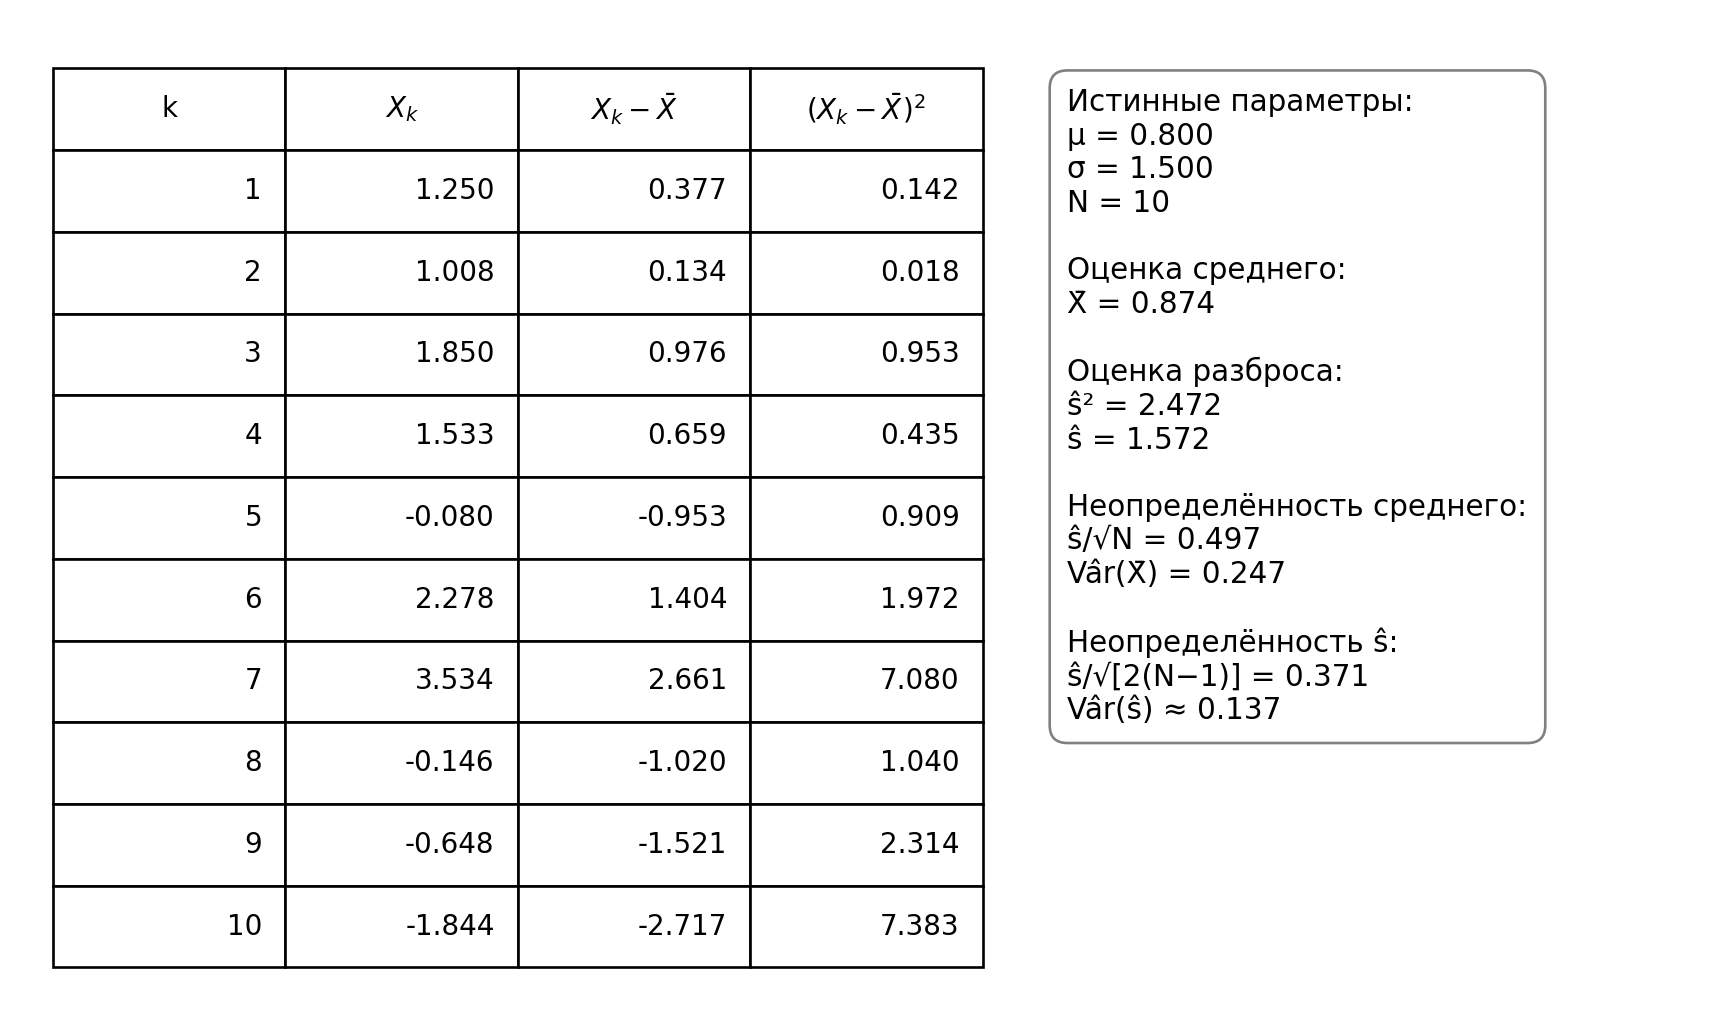
\includegraphics[keepaspectratio,alt={Один из возможных наборов десяти измерений для \textbackslash mu=0.8 и \textbackslash sigma=1.5. Вместе с исходными значениями показаны выборочное среднее, выборочная дисперсия и оценки неопределённостей.}]{chapters/../assets/figures/error_propagation_sample10.png}}

\end{center}

\BookInlineFigureCaption{Один из возможных наборов десяти измерений для \(\mu=0.8\) и
\(\sigma=1.5\). Вместе с исходными значениями показаны выборочное
среднее, выборочная дисперсия и оценки неопределённостей.}

\end{bookfigurepanel}

При изменении параметров или генерации новой выборки меняются и
\(\widehat\mu\), и \(\widehat\sigma\). Это наглядно подчёркивает, что
сами оценки являются случайными величинами.

\section{Несколько измеряемых
величин}\label{ux43dux435ux441ux43aux43eux43bux44cux43aux43e-ux438ux437ux43cux435ux440ux44fux435ux43cux44bux445-ux432ux435ux43bux438ux447ux438ux43d}

\subsection{Ошибка суммы двух
величин}\label{ux43eux448ux438ux431ux43aux430-ux441ux443ux43cux43cux44b-ux434ux432ux443ux445-ux432ux435ux43bux438ux447ux438ux43d}

Пусть

\[
S=X+Y.
\]

Тогда

\[
\begin{aligned}
\operatorname{Var}(S)
&=\mathbb E\!\left[
\bigl((X-\mu_X)+(Y-\mu_Y)\bigr)^2
\right]\\
&=\sigma_X^2+\sigma_Y^2+2\operatorname{Cov}(X,Y).
\end{aligned}
\]

Следовательно,

\[
\boxed{
\sigma_{X+Y}^2
=\sigma_X^2+\sigma_Y^2+2\operatorname{Cov}(X,Y).
}
\]

\subsection{Ковариация и коэффициент
корреляции}\label{ux43aux43eux432ux430ux440ux438ux430ux446ux438ux44f-ux438-ux43aux43eux44dux444ux444ux438ux446ux438ux435ux43dux442-ux43aux43eux440ux440ux435ux43bux44fux446ux438ux438}

\begin{booknote}

Ковариация двух случайных величин определяется как

\[
\boxed{
\operatorname{Cov}(X,Y)
=\mathbb E[(X-\mu_X)(Y-\mu_Y)].
}
\]

\begin{itemize}
\tightlist
\item
  \(\operatorname{Cov}(X,Y)>0\): величины обычно отклоняются в одну
  сторону;
\item
  \(\operatorname{Cov}(X,Y)<0\): отклонения обычно направлены в
  противоположные стороны;
\item
  \(\operatorname{Cov}(X,Y)=0\): линейной связи нет.
\end{itemize}

Независимость влечёт нулевую ковариацию, но нулевая ковариация сама по
себе в общем случае не означает независимость.

\end{booknote}

Чтобы убрать размерность ковариации, вводят коэффициент корреляции

\[
\boxed{
\rho_{XY}
=\frac{\operatorname{Cov}(X,Y)}{\sigma_X\sigma_Y},
\qquad
-1\le\rho_{XY}\le1.
}
\]

Тогда для суммы и разности

\[
\boxed{
\sigma_{X\pm Y}^2
=\sigma_X^2+\sigma_Y^2
\pm2\rho_{XY}\sigma_X\sigma_Y.
}
\]

Если \(\sigma_X=\sigma_Y=\sigma\), эти формулы особенно прозрачны:

\[
\sigma_{X+Y}^2=2\sigma^2(1+\rho),
\qquad
\sigma_{X-Y}^2=2\sigma^2(1-\rho).
\]

Положительная корреляция увеличивает ошибку суммы и уменьшает ошибку
разности; отрицательная корреляция действует противоположным образом.
Именно из-за этого нельзя автоматически складывать все ошибки в
квадратуре.

\subsection{Как оценить корреляцию по
выборке}\label{ux43aux430ux43a-ux43eux446ux435ux43dux438ux442ux44c-ux43aux43eux440ux440ux435ux43bux44fux446ux438ux44e-ux43fux43e-ux432ux44bux431ux43eux440ux43aux435}

Для наблюдений \((x_k,y_k)\), \(k=1,\ldots,N\), выборочная ковариация
оценивается как

\[
\widehat{\operatorname{Cov}}(X,Y)
=
\frac{1}{N-1}
\sum_{k=1}^{N}
(x_k-\langle x\rangle)(y_k-\langle y\rangle),
\]

а коэффициент корреляции --- как

\[
\boxed{
\widehat\rho
=
\frac{\widehat{\operatorname{Cov}}(X,Y)}{s_Xs_Y}.
}
\]

При небольшом числе наблюдений сама оценка \(\widehat\rho\) может
заметно флуктуировать. Корреляцию можно определять по данным или по
моделированию отклика детектора.

\subsection{Общая формула распространения
ошибки}\label{ux43eux431ux449ux430ux44f-ux444ux43eux440ux43cux443ux43bux430-ux440ux430ux441ux43fux440ux43eux441ux442ux440ux430ux43dux435ux43dux438ux44f-ux43eux448ux438ux431ux43aux438}

Пусть

\[
F=f(X_1,\ldots,X_n).
\]

В первом порядке разложения около средних значений

\[
F-\mathbb E[F]
\approx
\sum_i
\frac{\partial f}{\partial x_i}
(X_i-\mu_i).
\]

\begin{bookderivation}

\subsubsection{Вывод общей
формулы}\label{ux432ux44bux432ux43eux434-ux43eux431ux449ux435ux439-ux444ux43eux440ux43cux443ux43bux44b}

Обозначим

\[
f_i=\left.\frac{\partial f}{\partial x_i}\right|_{\mathbf x=\boldsymbol\mu}.
\]

Тогда

\[
F-\mathbb E[F]\approx\sum_i f_i(X_i-\mu_i).
\]

Возводя в квадрат и усредняя,

\[
\begin{aligned}
\operatorname{Var}(F)
&\approx
\mathbb E\!\left[
\left(\sum_i f_i(X_i-\mu_i)\right)
\left(\sum_j f_j(X_j-\mu_j)\right)
\right]\\
&=
\sum_{i,j}f_i f_j
\mathbb E[(X_i-\mu_i)(X_j-\mu_j)].
\end{aligned}
\]

По определению ковариации получаем

\[
\boxed{
\operatorname{Var}(F)
\approx
\sum_{i,j}
\frac{\partial f}{\partial x_i}
\operatorname{Cov}(X_i,X_j)
\frac{\partial f}{\partial x_j}.
}
\quad\blacksquare
\]

\end{bookderivation}

Для двух переменных \(F=f(X,Y)\) формула принимает вид

\[
\boxed{
\begin{aligned}
\sigma_F^2\approx{}&
\left(\frac{\partial f}{\partial x}\right)^2\sigma_X^2
+\left(\frac{\partial f}{\partial y}\right)^2\sigma_Y^2\\
&+2\rho_{XY}
\frac{\partial f}{\partial x}
\frac{\partial f}{\partial y}
\sigma_X\sigma_Y.
\end{aligned}
}
\]

Все производные вычисляются в точке центральных значений.

\subsection{Интерактив: вклад корреляции в
дисперсию}\label{ux438ux43dux442ux435ux440ux430ux43aux442ux438ux432-ux432ux43aux43bux430ux434-ux43aux43eux440ux440ux435ux43bux44fux446ux438ux438-ux432-ux434ux438ux441ux43fux435ux440ux441ux438ux44e}

\begin{bookfigurepanel}

\begin{center}

\pandocbounded{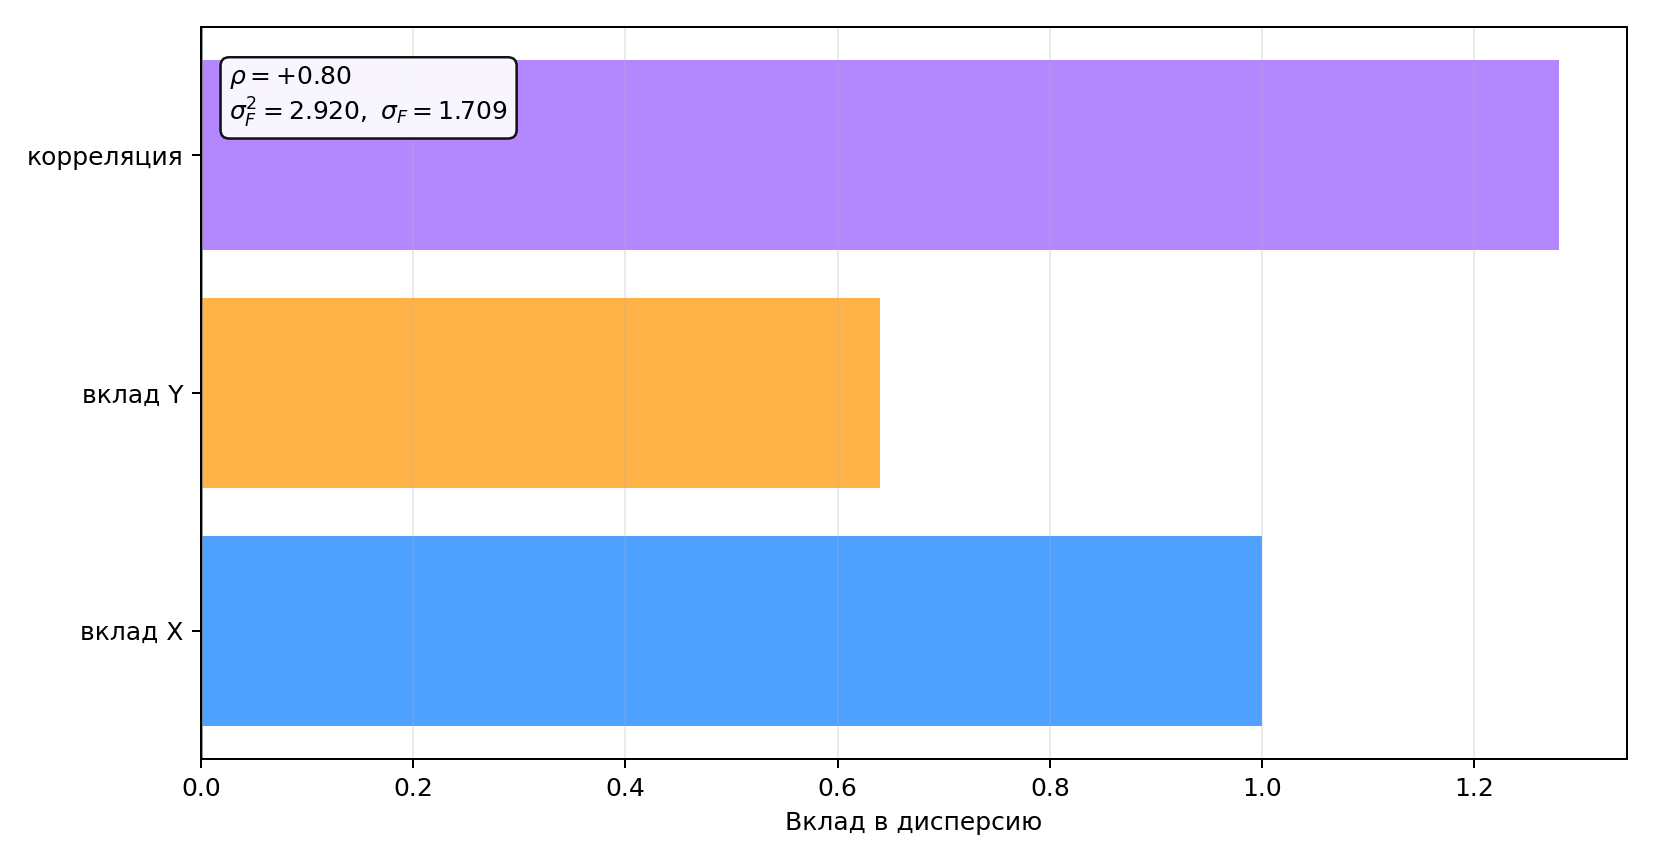
\includegraphics[keepaspectratio,alt={При положительной корреляции \textbackslash rho=0.8 корреляционный член увеличивает итоговую дисперсию для производных одного знака.}]{chapters/../assets/figures/error_propagation_corr_positive.png}}

\end{center}

\BookInlineFigureCaption{При положительной корреляции \(\rho=0.8\) корреляционный член
увеличивает итоговую дисперсию для производных одного знака.}

\end{bookfigurepanel}

\begin{bookfigurepanel}

\begin{center}

\pandocbounded{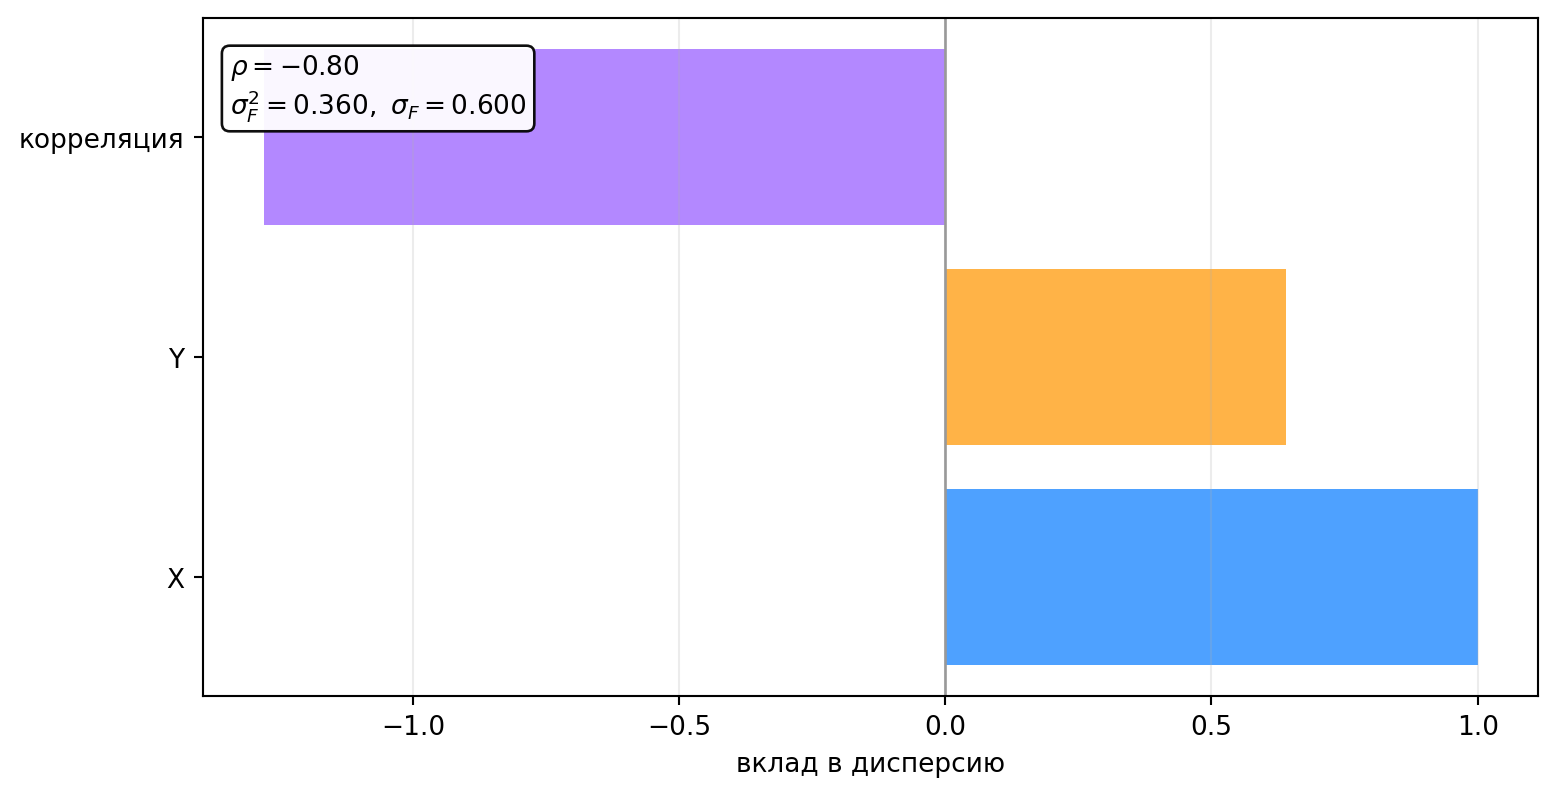
\includegraphics[keepaspectratio,alt={При отрицательной корреляции \textbackslash rho=-0.8 тот же корреляционный член вычитается из дисперсии и уменьшает итоговую ошибку.}]{chapters/../assets/figures/error_propagation_corr_negative.png}}

\end{center}

\BookInlineFigureCaption{При отрицательной корреляции \(\rho=-0.8\) тот же корреляционный член
вычитается из дисперсии и уменьшает итоговую ошибку.}

\end{bookfigurepanel}

\subsection{Пример: отношение двух
величин}\label{ux43fux440ux438ux43cux435ux440-ux43eux442ux43dux43eux448ux435ux43dux438ux435-ux434ux432ux443ux445-ux432ux435ux43bux438ux447ux438ux43d}

Для

\[R=\frac{X}{Y}\]

имеем

\[
\frac{\partial R}{\partial X}=\frac1Y,
\qquad
\frac{\partial R}{\partial Y}=-\frac{X}{Y^2}.
\]

После подстановки в общую формулу получаем

\[
\boxed{
\left(\frac{\sigma_R}{R}\right)^2
\approx
\left(\frac{\sigma_X}{X}\right)^2
+
\left(\frac{\sigma_Y}{Y}\right)^2
-
2\rho_{XY}
\frac{\sigma_X}{X}
\frac{\sigma_Y}{Y}.
}
\]

Для отношения положительная корреляция уменьшает ошибку, поскольку
производные по числителю и знаменателю имеют противоположные знаки.

\section{Ковариационная
матрица}\label{ux43aux43eux432ux430ux440ux438ux430ux446ux438ux43eux43dux43dux430ux44f-ux43cux430ux442ux440ux438ux446ux430}

Для случайного вектора

\[
\mathbf X=(X_1,\ldots,X_n)^T
\]

ковариационная матрица определяется элементами

\[
\boxed{
V_{ij}=\operatorname{Cov}(X_i,X_j).
}
\]

Для двух величин

\[
\boxed{
V=
\begin{pmatrix}
\sigma_X^2&\rho\sigma_X\sigma_Y\\
\rho\sigma_X\sigma_Y&\sigma_Y^2
\end{pmatrix}.
}
\]

\begin{booknote}

Ковариационная матрица обладает тремя важными свойствами:

\begin{enumerate}
\def\labelenumi{\arabic{enumi}.}
\tightlist
\item
  \(V\) симметрична: \(V_{ij}=V_{ji}\);
\item
  на диагонали стоят дисперсии \(V_{ii}=\operatorname{Var}(X_i)\);
\item
  для любого вектора \(\mathbf a\) выполняется
  \(\mathbf a^TV\mathbf a\ge0\), то есть \(V\) положительно
  полуопределена.
\end{enumerate}

\end{booknote}

Последнее свойство имеет непосредственный статистический смысл:

\[
\begin{aligned}
\mathbf a^TV\mathbf a
&=
\mathbb E\!\left[
\left(\mathbf a^T(\mathbf X-\boldsymbol\mu)\right)^2
\right]\\
&=
\operatorname{Var}(\mathbf a^T\mathbf X)
\ge0.
\end{aligned}
\]

\subsection{Матричная запись распространения
ошибки}\label{ux43cux430ux442ux440ux438ux447ux43dux430ux44f-ux437ux430ux43fux438ux441ux44c-ux440ux430ux441ux43fux440ux43eux441ux442ux440ux430ux43dux435ux43dux438ux44f-ux43eux448ux438ux431ux43aux438}

Введём градиент

\[
\nabla f
=
\begin{pmatrix}
\partial f/\partial x_1\\
\vdots\\
\partial f/\partial x_n
\end{pmatrix}.
\]

Тогда общая формула распространения принимает компактный вид

\[
\boxed{
\sigma_f^2
\approx
(\nabla f)^TV(\nabla f).
}
\]

Если выходных величин несколько,

\[
\mathbf Y=\mathbf f(\mathbf X),
\]

то вводится матрица Якоби

\[
J_{ai}=\frac{\partial f_a}{\partial x_i}.
\]

Универсальный закон линейного преобразования ковариационной матрицы:

\[
\boxed{
V_Y\approx JV_XJ^T.
}
\]

\subsection{Пример: сумма и
разность}\label{ux43fux440ux438ux43cux435ux440-ux441ux443ux43cux43cux430-ux438-ux440ux430ux437ux43dux43eux441ux442ux44c}

Пусть

\[
\mathbf X=
\begin{pmatrix}X\\Y\end{pmatrix},
\qquad
\mathbf U=
\begin{pmatrix}S\\D\end{pmatrix}
=
\begin{pmatrix}X+Y\\X-Y\end{pmatrix}.
\]

Матрица Якоби равна

\[
J=
\begin{pmatrix}
1&1\\
1&-1
\end{pmatrix}.
\]

Для

\[
V_X=
\begin{pmatrix}
\sigma_X^2&\sigma_{XY}\\
\sigma_{XY}&\sigma_Y^2
\end{pmatrix}
\]

получаем

\[
\boxed{
V_U
=JV_XJ^T
=
\begin{pmatrix}
\sigma_X^2+\sigma_Y^2+2\sigma_{XY}&\sigma_X^2-\sigma_Y^2\\
\sigma_X^2-\sigma_Y^2&\sigma_X^2+\sigma_Y^2-2\sigma_{XY}
\end{pmatrix}.
}
\]

Из внедиагонального элемента видно, что

\[
\operatorname{Cov}(S,D)=\sigma_X^2-\sigma_Y^2.
\]

Если \(\sigma_X=\sigma_Y\), сумма и разность оказываются
некоррелированными.

\section{Двумерное гауссово
распределение}\label{ux434ux432ux443ux43cux435ux440ux43dux43eux435-ux433ux430ux443ux441ux441ux43eux432ux43e-ux440ux430ux441ux43fux440ux435ux434ux435ux43bux435ux43dux438ux435}

Ковариационная матрица не только переносит ошибки. Для гауссовских
случайных величин она определяет всю геометрию совместного
распределения.

\subsection{Независимые гауссовы
величины}\label{ux43dux435ux437ux430ux432ux438ux441ux438ux43cux44bux435-ux433ux430ux443ux441ux441ux43eux432ux44b-ux432ux435ux43bux438ux447ux438ux43dux44b}

Пусть

\[
X\sim\mathrm N(\mu_X,\sigma_X^2),
\qquad
Y\sim\mathrm N(\mu_Y,\sigma_Y^2)
\]

независимы. Тогда совместная плотность равна произведению одномерных
плотностей:

\[
\boxed{
f(x,y)
=
\frac{1}{2\pi\sigma_X\sigma_Y}
\exp\!\left[
-\frac12\left(
\frac{(x-\mu_X)^2}{\sigma_X^2}
+
\frac{(y-\mu_Y)^2}{\sigma_Y^2}
\right)
\right].
}
\]

Линии постоянной плотности --- эллипсы с осями вдоль координатных осей.

\subsection{Коррелированный
случай}\label{ux43aux43eux440ux440ux435ux43bux438ux440ux43eux432ux430ux43dux43dux44bux439-ux441ux43bux443ux447ux430ux439}

Введём безразмерные отклонения

\[
u=\frac{x-\mu_X}{\sigma_X},
\qquad
v=\frac{y-\mu_Y}{\sigma_Y}.
\]

Для независимых переменных экспонента содержит \(u^2+v^2\). При наличии
корреляции появляется смешанный член:

\[
\boxed{
Q_\rho(u,v)
=
\frac{u^2-2\rho uv+v^2}{1-\rho^2},
\qquad
|\rho|<1.
}
\]

Соответствующая совместная плотность равна

\[
\boxed{
f(x,y)
=
\frac{1}{2\pi\sigma_X\sigma_Y\sqrt{1-\rho^2}}
\exp\!\left[
-\frac12
\frac{u^2-2\rho uv+v^2}{1-\rho^2}
\right].
}
\]

Знак \(\rho\) задаёт направление наклона облака точек, а модуль
корреляции --- степень его вытянутости.

\subsection{Та же формула через ковариационную
матрицу}\label{ux442ux430-ux436ux435-ux444ux43eux440ux43cux443ux43bux430-ux447ux435ux440ux435ux437-ux43aux43eux432ux430ux440ux438ux430ux446ux438ux43eux43dux43dux443ux44e-ux43cux430ux442ux440ux438ux446ux443}

Для

\[
V=
\begin{pmatrix}
\sigma_X^2&\rho\sigma_X\sigma_Y\\
\rho\sigma_X\sigma_Y&\sigma_Y^2
\end{pmatrix}
\]

определитель и обратная матрица равны

\[
\det V=\sigma_X^2\sigma_Y^2(1-\rho^2),
\]

\[
V^{-1}
=
\frac{1}{1-\rho^2}
\begin{pmatrix}
1/\sigma_X^2&-\rho/(\sigma_X\sigma_Y)\\
-\rho/(\sigma_X\sigma_Y)&1/\sigma_Y^2
\end{pmatrix}.
\]

Если

\[
\boldsymbol\delta
=
\begin{pmatrix}
x-\mu_X\\
y-\mu_Y
\end{pmatrix},
\]

то

\[
\boxed{
\boldsymbol\delta^TV^{-1}\boldsymbol\delta
=
\frac{u^2-2\rho uv+v^2}{1-\rho^2}.
}
\]

Таким образом, запись через коэффициент корреляции и запись через
\(V^{-1}\) полностью эквивалентны.

\subsection{\texorpdfstring{Почему \(\rho\) действительно является
корреляцией}{Почему \textbackslash rho действительно является корреляцией}}\label{ux43fux43eux447ux435ux43cux443-rho-ux434ux435ux439ux441ux442ux432ux438ux442ux435ux43bux44cux43dux43e-ux44fux432ux43bux44fux435ux442ux441ux44f-ux43aux43eux440ux440ux435ux43bux44fux446ux438ux435ux439}

Возьмём независимые стандартные гауссовы величины

\[
Z_1,Z_2\sim\mathrm N(0,1),
\qquad
\operatorname{Cov}(Z_1,Z_2)=0,
\]

и построим

\[
X=\mu_X+\sigma_XZ_1,
\]

\[
Y=\mu_Y+\sigma_Y\left(\rho Z_1+\sqrt{1-\rho^2}Z_2\right).
\]

\begin{bookderivation}

\subsubsection{Восстановление дисперсий и
ковариации}\label{ux432ux43eux441ux441ux442ux430ux43dux43eux432ux43bux435ux43dux438ux435-ux434ux438ux441ux43fux435ux440ux441ux438ux439-ux438-ux43aux43eux432ux430ux440ux438ux430ux446ux438ux438}

Для \(X\) сразу получаем

\[
\mathbb E[X]=\mu_X,
\qquad
\operatorname{Var}(X)=\sigma_X^2.
\]

Для \(Y\)

\[
\mathbb E[Y]=\mu_Y
\]

и, используя независимость \(Z_1\) и \(Z_2\),

\[
\begin{aligned}
\operatorname{Var}(Y)
&=\sigma_Y^2\left[
\rho^2\operatorname{Var}(Z_1)
+(1-\rho^2)\operatorname{Var}(Z_2)
\right]\\
&=\sigma_Y^2[\rho^2+(1-\rho^2)]
=\sigma_Y^2.
\end{aligned}
\]

Ковариация равна

\[
\begin{aligned}
\operatorname{Cov}(X,Y)
&=\sigma_X\sigma_Y
\operatorname{Cov}\!\left(
Z_1,
\rho Z_1+\sqrt{1-\rho^2}Z_2
\right)\\
&=\rho\sigma_X\sigma_Y.
\end{aligned}
\]

Следовательно,

\[
\boxed{
\rho=
\frac{\operatorname{Cov}(X,Y)}{\sigma_X\sigma_Y}.
}
\quad\blacksquare
\]

\end{bookderivation}

\subsection{Произвольная размерность и расстояние
Махаланобиса}\label{ux43fux440ux43eux438ux437ux432ux43eux43bux44cux43dux430ux44f-ux440ux430ux437ux43cux435ux440ux43dux43eux441ux442ux44c-ux438-ux440ux430ux441ux441ux442ux43eux44fux43dux438ux435-ux43cux430ux445ux430ux43bux430ux43dux43eux431ux438ux441ux430}

В \(d\) измерениях гауссовская плотность записывается как

\[
\boxed{
f(\mathbf x)
=
\frac{1}{(2\pi)^{d/2}\sqrt{\det V}}
\exp\!\left[
-\frac12
(\mathbf x-\boldsymbol\mu)^T
V^{-1}
(\mathbf x-\boldsymbol\mu)
\right].
}
\]

Величина

\[
\boxed{
D^2
=(\mathbf x-\boldsymbol\mu)^T
V^{-1}
(\mathbf x-\boldsymbol\mu)
}
\]

называется квадратом расстояния Махаланобиса.

\begin{booknote}

Контуры \(D^2=c\) являются эллипсами в двух измерениях и эллипсоидами в
большей размерности. Собственные векторы \(V\) задают направления
главных осей, а собственные значения --- квадраты характерных масштабов
вдоль этих осей. Корреляция проявляется как поворот эллипса относительно
исходных координат.

\end{booknote}

\subsection{Интерактив: корреляция и
эллипс}\label{ux438ux43dux442ux435ux440ux430ux43aux442ux438ux432-ux43aux43eux440ux440ux435ux43bux44fux446ux438ux44f-ux438-ux44dux43bux43bux438ux43fux441}

\begin{bookfigurepanel}

\begin{center}

\pandocbounded{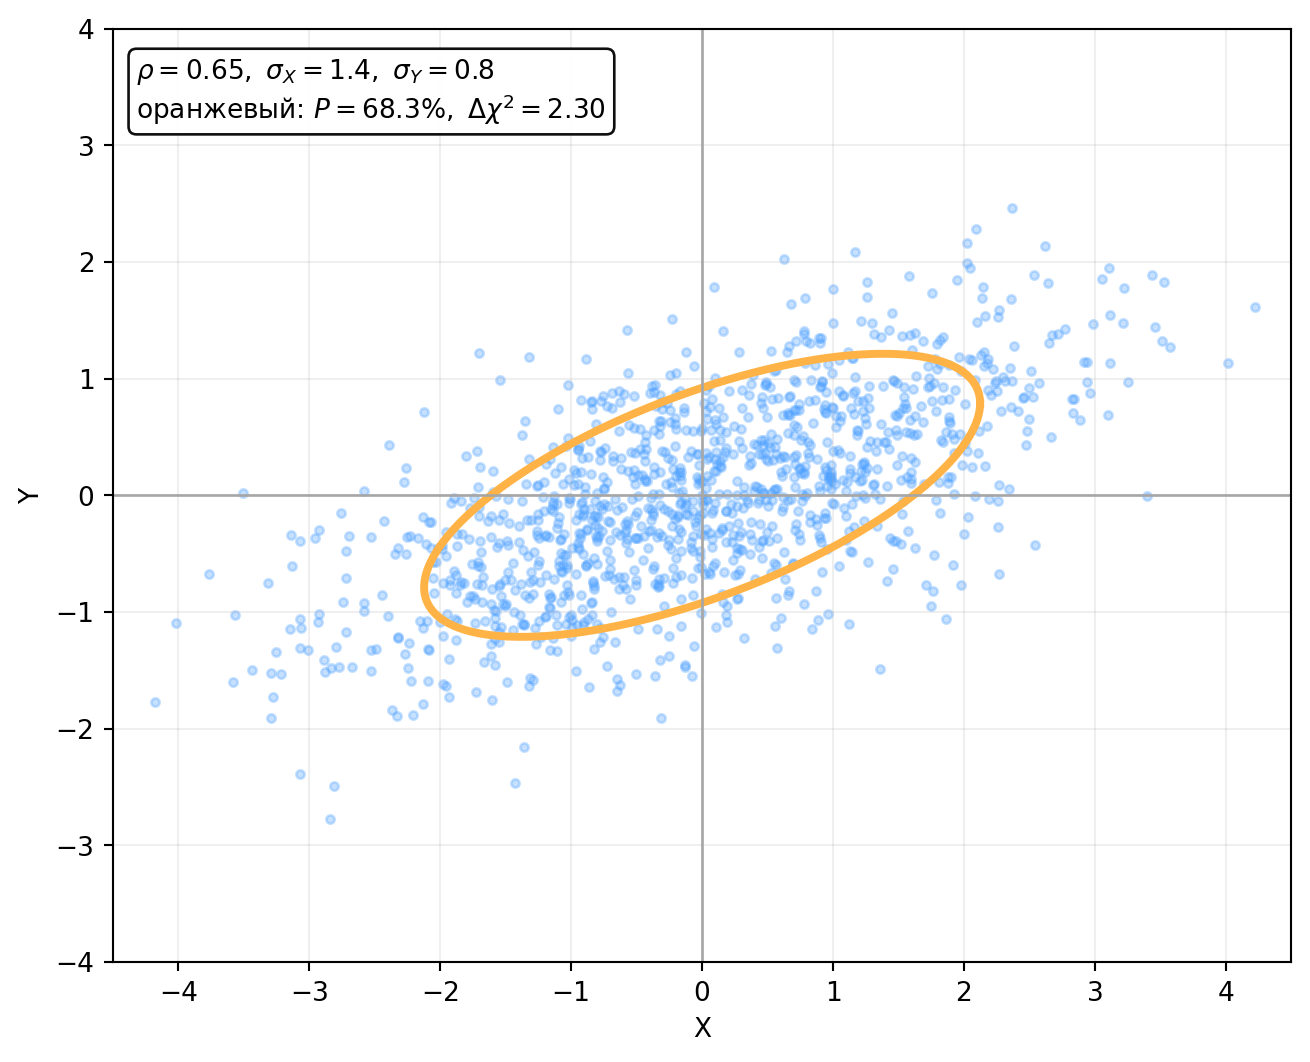
\includegraphics[keepaspectratio,alt={Облако коррелированных гауссовских точек при \textbackslash rho=0.65. Оранжевый эллипс соответствует области с вероятностью 68.3\textbackslash\%, то есть \textbackslash Delta\textbackslash chi\^{}2=2.30 в двумерном случае.}]{chapters/../assets/figures/gaussian2d_correlation_ellipse.png}}

\end{center}

\BookInlineFigureCaption{Облако коррелированных гауссовских точек при \(\rho=0.65\). Оранжевый
эллипс соответствует области с вероятностью \(68.3\%\), то есть
\(\Delta\chi^2=2.30\) в двумерном случае.}

\end{bookfigurepanel}

\section{Эллипсы и вероятностные
контуры}\label{ux44dux43bux43bux438ux43fux441ux44b-ux438-ux432ux435ux440ux43eux44fux442ux43dux43eux441ux442ux43dux44bux435-ux43aux43eux43dux442ux443ux440ux44b}

\subsection{Одномерный и двумерный случаи
различаются}\label{ux43eux434ux43dux43eux43cux435ux440ux43dux44bux439-ux438-ux434ux432ux443ux43cux435ux440ux43dux44bux439-ux441ux43bux443ux447ux430ux438-ux440ux430ux437ux43bux438ux447ux430ux44eux442ux441ux44f}

Для стандартного одномерного гаусса

\[
P(|Z|\le1)=0.683.
\]

В двумерном стандартном гауссе область

\[
X^2+Y^2\le1
\]

содержит только

\[
\boxed{
P(D^2\le1)=1-e^{-1/2}\approx0.393.
}
\]

\begin{booknote}

Контур «одна сигма по радиусу» в двух измерениях не является областью с
вероятностью \(68.3\%\). Вероятностный уровень контура зависит от
размерности пространства.

\end{booknote}

Для двумерного гаусса

\[
D^2
=(\mathbf x-\boldsymbol\mu)^TV^{-1}(\mathbf x-\boldsymbol\mu)
\sim\chi_2^2.
\]

Отсюда вероятность оказаться внутри контура \(D^2\le c\) равна

\[
\boxed{
P(D^2\le c)=1-e^{-c/2}.
}
\]

Обратная зависимость имеет вид

\[
\boxed{
c=-2\ln(1-P).
}
\]

Практически полезные уровни:

{\def\LTcaptype{none} % do not increment counter
\begin{longtable}[]{@{}rr@{}}
\toprule\noalign{}
Вероятность внутри контура & \(c=\Delta\chi^2\) \\
\midrule\noalign{}
\endhead
\bottomrule\noalign{}
\endlastfoot
\(39.3\%\) & \(1.00\) \\
\(68.3\%\) & \(2.30\) \\
\(90\%\) & \(4.61\) \\
\(95\%\) & \(5.99\) \\
\(99\%\) & \(9.21\) \\
\end{longtable}
}

\subsection{Интерактив: вероятность и размер
контура}\label{ux438ux43dux442ux435ux440ux430ux43aux442ux438ux432-ux432ux435ux440ux43eux44fux442ux43dux43eux441ux442ux44c-ux438-ux440ux430ux437ux43cux435ux440-ux43aux43eux43dux442ux443ux440ux430}

\begin{bookfigurepanel}

\begin{center}

\pandocbounded{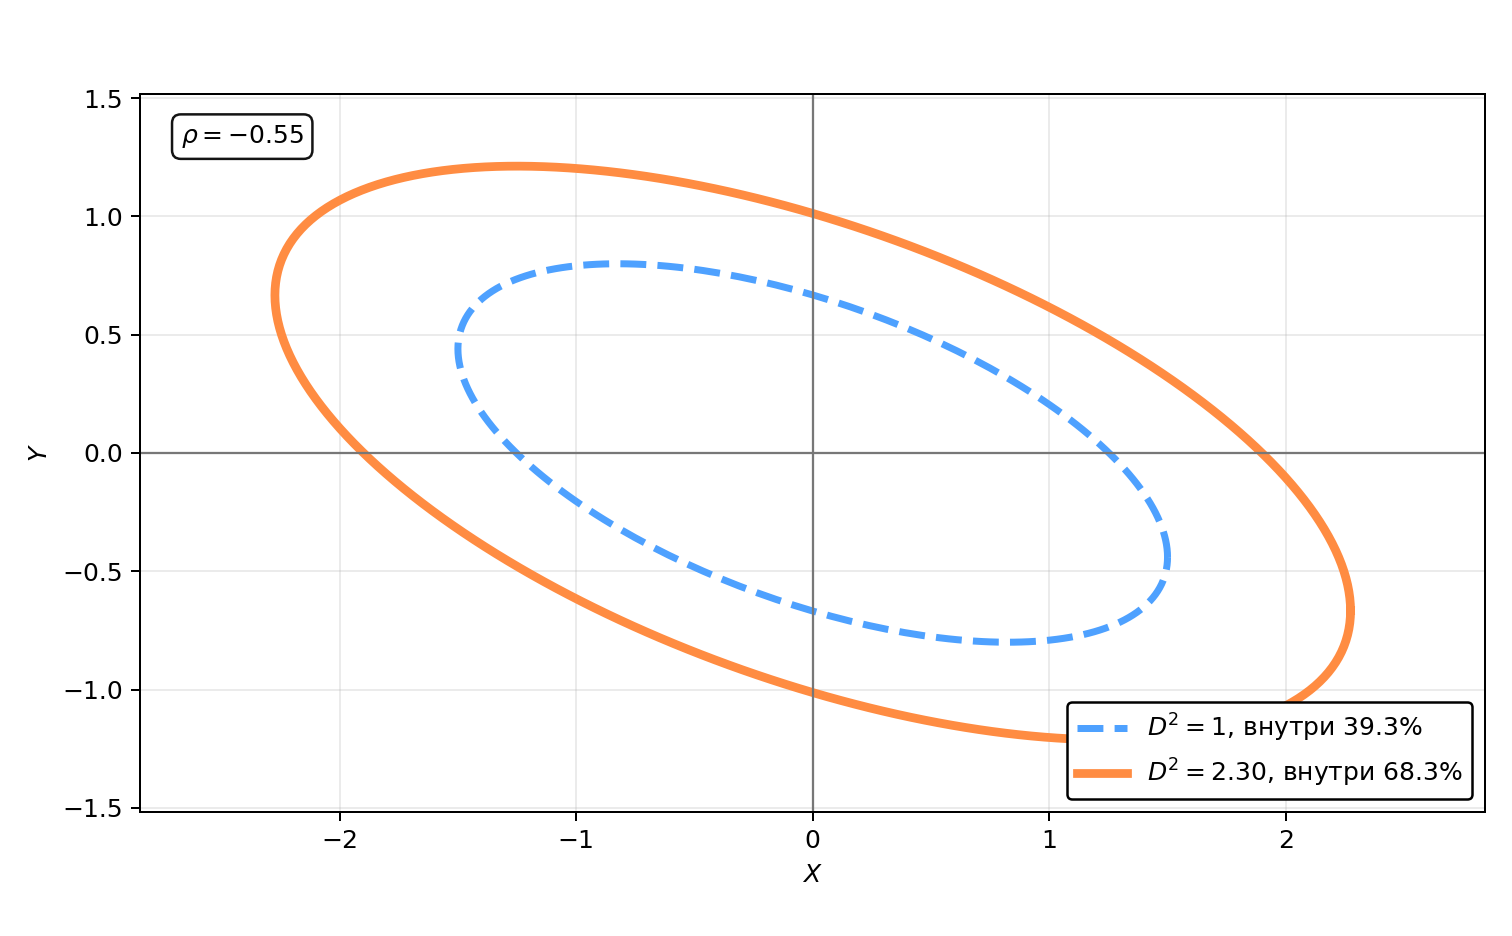
\includegraphics[keepaspectratio,alt={Два двумерных гауссовских контура при одинаковой корреляции: голубой пунктир отвечает \textbackslash Delta\textbackslash chi\^{}2=1 и содержит 39.3\textbackslash\% вероятности, оранжевый контур с \textbackslash Delta\textbackslash chi\^{}2=2.30 --- 68.3\textbackslash\%.}]{chapters/../assets/figures/gaussian2d_probability_contour.png}}

\end{center}

\BookInlineFigureCaption{Два двумерных гауссовских контура при одинаковой корреляции: голубой
пунктир отвечает \(\Delta\chi^2=1\) и содержит \(39.3\%\) вероятности,
оранжевый контур с \(\Delta\chi^2=2.30\) --- \(68.3\%\).}

\end{bookfigurepanel}

\subsection{Контур распределения и контур
параметров}\label{ux43aux43eux43dux442ux443ux440-ux440ux430ux441ux43fux440ux435ux434ux435ux43bux435ux43dux438ux44f-ux438-ux43aux43eux43dux442ux443ux440-ux43fux430ux440ux430ux43cux435ux442ux440ux43eux432}

Здесь эллипс описывает распределение известного случайного вектора
\(\mathbf X\). В задачах оценивания параметров похожие контуры строятся
вокруг best fit уже в пространстве параметров. Формулы часто имеют
похожую квадратичную форму, но вероятностная интерпретация контуров
параметров требует дополнительных условий и рассматривается отдельно
вместе с likelihood и методом \(\chi^2\).

\section{Практические
применения}\label{ux43fux440ux430ux43aux442ux438ux447ux435ux441ux43aux438ux435-ux43fux440ux438ux43cux435ux43dux435ux43dux438ux44f}

\subsection{Усреднение независимых
измерений}\label{ux443ux441ux440ux435ux434ux43dux435ux43dux438ux435-ux43dux435ux437ux430ux432ux438ux441ux438ux43cux44bux445-ux438ux437ux43cux435ux440ux435ux43dux438ux439}

Пусть независимые измерения одной и той же величины равны

\[
x_i\pm\sigma_i.
\]

Оптимальное взвешенное среднее записывается как

\[
\boxed{
\widehat\mu
=
\frac{\sum_i x_i/\sigma_i^2}{\sum_i1/\sigma_i^2},
\qquad
\sigma_{\widehat\mu}^2
=
\frac{1}{\sum_i1/\sigma_i^2}.
}
\]

Измерение с меньшей дисперсией получает больший вес.

\subsection{Усреднение коррелированных
измерений}\label{ux443ux441ux440ux435ux434ux43dux435ux43dux438ux435-ux43aux43eux440ux440ux435ux43bux438ux440ux43eux432ux430ux43dux43dux44bux445-ux438ux437ux43cux435ux440ux435ux43dux438ux439}

Если измерения собраны в вектор \(\mathbf x\) и имеют ковариационную
матрицу \(V\), то обобщение взвешенного среднего имеет вид

\[
\boxed{
\widehat\mu
=
\frac{\mathbf1^TV^{-1}\mathbf x}{\mathbf1^TV^{-1}\mathbf1},
\qquad
\sigma_{\widehat\mu}^2
=
\frac{1}{\mathbf1^TV^{-1}\mathbf1}.
}
\]

Коррелированная информация не должна учитываться несколько раз. При
сильных корреляциях отдельные веса в такой комбинации могут оказаться
отрицательными.

\subsection{Пример: инвариантная масса двух
частиц}\label{ux43fux440ux438ux43cux435ux440-ux438ux43dux432ux430ux440ux438ux430ux43dux442ux43dux430ux44f-ux43cux430ux441ux441ux430-ux434ux432ux443ux445-ux447ux430ux441ux442ux438ux446}

Для двух безмассовых частиц

\[
m^2=2E_1E_2(1-\cos\theta).
\]

Удобно сначала распространить ошибку на \(m^2\). Градиент равен

\[
\nabla m^2
=
\begin{pmatrix}
2E_2(1-\cos\theta)\\
2E_1(1-\cos\theta)\\
2E_1E_2\sin\theta
\end{pmatrix},
\]

а дисперсия

\[
\sigma_{m^2}^2
\approx
(\nabla m^2)^TV(\nabla m^2).
\]

После этого

\[
\sigma_m\approx\frac{\sigma_{m^2}}{2m}.
\]

Рассмотрим численный пример:

\[
E_1=60.0~\mathrm{GeV},
\qquad
E_2=40.0~\mathrm{GeV},
\qquad
\theta=0.200~\mathrm{rad},
\]

\[
V_x=
\begin{pmatrix}
1.44&0.36&0\\
0.36&1.00&0\\
0&0&2.5\cdot10^{-5}
\end{pmatrix}.
\]

\begin{bookderivation}

\subsubsection{Распространение ковариационной матрицы на инвариантную
массу}\label{ux440ux430ux441ux43fux440ux43eux441ux442ux440ux430ux43dux435ux43dux438ux435-ux43aux43eux432ux430ux440ux438ux430ux446ux438ux43eux43dux43dux43eux439-ux43cux430ux442ux440ux438ux446ux44b-ux43dux430-ux438ux43dux432ux430ux440ux438ux430ux43dux442ux43dux443ux44e-ux43cux430ux441ux441ux443}

Сначала вычислим

\[
m^2
=2\cdot60\cdot40\cdot(1-\cos0.200)
=95.680~\mathrm{GeV}^2,
\]

откуда

\[
m=\sqrt{m^2}=9.782~\mathrm{GeV}.
\]

Градиент в заданной точке:

\[
\nabla m^2
=
\begin{pmatrix}
1.595\\
2.392\\
953.613
\end{pmatrix}.
\]

Подставляя его в квадратичную форму, получаем

\[
\operatorname{Var}(m^2)
\approx
(\nabla m^2)^TV_x(\nabla m^2)
=34.864~\mathrm{GeV}^4.
\]

Следовательно,

\[
\sigma_{m^2}
=\sqrt{34.864}
=5.905~\mathrm{GeV}^2,
\]

и

\[
\sigma_m
\approx
\frac{5.905}{2\cdot9.782}
=0.302~\mathrm{GeV}.
\]

Итог можно записать двумя эквивалентными способами:

\[
\boxed{
m^2=95.68\pm5.91~\mathrm{GeV}^2
}
\]

или

\[
\boxed{
m=9.78\pm0.30~\mathrm{GeV}.
}
\quad\blacksquare
\]

\end{bookderivation}

\section{Аналитическая формула или
Монте-Карло}\label{ux430ux43dux430ux43bux438ux442ux438ux447ux435ux441ux43aux430ux44f-ux444ux43eux440ux43cux443ux43bux430-ux438ux43bux438-ux43cux43eux43dux442ux435-ux43aux430ux440ux43bux43e}

Линейное распространение ошибок быстро, прозрачно и особенно удобно при
работе с ковариационными матрицами. Оно хорошо работает при малых почти
гауссовских ошибках и слабой нелинейности. При сильной нелинейности,
заметной асимметрии, физических границах или произвольной форме входных
распределений аналитическое линейное приближение может перестать быть
достаточным.

Метод Монте-Карло позволяет непосредственно генерировать входные
случайные величины с нужными распределениями и корреляциями, пропускать
их через функцию \(\mathbf f\) и получать распределение результата без
принудительной линеаризации. Он требует больше вычислений и полной
модели входных ошибок, но сохраняет нелинейность, асимметрию и
физические границы.

\begin{booknote}

Практическая последовательность проверки результата:

\begin{enumerate}
\def\labelenumi{\arabic{enumi}.}
\tightlist
\item
  Записать функцию \(\mathbf Y=\mathbf f(\mathbf X)\).
\item
  Перечислить все источники неопределённости.
\item
  Построить полную ковариационную матрицу \(V_X\).
\item
  Вычислить Якобиан \(J\).
\item
  Получить \(V_Y\approx JV_XJ^T\).
\item
  Проверить единицы измерения и предельные случаи.
\item
  При заметной нелинейности сравнить аналитический результат с
  Монте-Карло.
\item
  Сохранять и публиковать ковариационную матрицу вместе с результатом.
\end{enumerate}

\end{booknote}

Типичные ошибки анализа --- складывать все неопределённости в квадратуре
без проверки корреляций, путать нулевую корреляцию с независимостью,
использовать относительные ошибки рядом с нулём, линеаризовать функцию
около неверной точки, считать ошибку симметричной после сильного
нелинейного преобразования, называть \(\Delta\chi^2=1\) областью
\(68\%\) независимо от размерности и публиковать только диагональные
ошибки без ковариаций.

\begin{bookchaptersummary}[Итоги главы]

\begin{itemize}
\tightlist
\item
  Ошибка производной величины определяется локальной чувствительностью
  функции к исходным измерениям; для одной переменной
  \(\sigma_Y\approx|f'(\mu_X)|\sigma_X\).
\item
  Линейное распространение работает только тогда, когда функцию
  действительно можно заменить касательной на масштабе входной
  неопределённости.
\item
  Оценки среднего, дисперсии и стандартного отклонения сами флуктуируют
  от выборки к выборке; для гауссовой выборки
  \(\operatorname{Var}(\widehat{\sigma^2})=2\sigma^4/(N-1)\), а при
  большом \(N\) относительный разброс \(\widehat\sigma\) имеет порядок
  \(1/\sqrt{2(N-1)}\).
\item
  Ковариация и коэффициент корреляции необходимы для корректного
  распространения связанных неопределённостей; знак корреляции может как
  увеличивать, так и уменьшать ошибку производной величины.
\item
  Ковариационная матрица объединяет все дисперсии и ковариации, а общий
  закон линейного преобразования имеет вид \(V_Y\approx JV_XJ^T\).
\item
  Та же матрица определяет геометрию многомерного гаусса: квадратичная
  форма \((\mathbf x-\boldsymbol\mu)^TV^{-1}(\mathbf x-\boldsymbol\mu)\)
  задаёт расстояние Махаланобиса и эллиптические контуры равной
  плотности.
\item
  В двух измерениях \(\Delta\chi^2=1\) содержит только \(39.3\%\)
  вероятности; область \(68.3\%\) соответствует \(\Delta\chi^2=2.30\).
\item
  При заметной нелинейности аналитическое распространение нужно
  проверять моделированием Монте-Карло.
\end{itemize}

\end{bookchaptersummary}

\section{Материалы
курса}\label{ux43cux430ux442ux435ux440ux438ux430ux43bux44b-ux43aux443ux440ux441ux430-3}

\begin{itemize}
\tightlist
\item
  \href{https://neutrinohit.github.io/statistical-analysis-course/ru/slides/05_error_propagation.html}{Слайды:
  распространение ошибок}
\item
  \href{https://neutrinohit.github.io/statistical-analysis-course/ru/slides/06_two_dimensional_gaussian.html}{Слайды:
  двумерный гаусс}
\item
  \href{https://neutrinohit.github.io/statistical-analysis-course/ru/slides/exercises/05_error_propagation_and_covariance_exercises.html}{Задачи}
\end{itemize}

\chapter{Метод Монте-Карло и
псевдоэксперименты}\label{ux43cux435ux442ux43eux434-ux43cux43eux43dux442ux435-ux43aux430ux440ux43bux43e-ux438-ux43fux441ux435ux432ux434ux43eux44dux43aux441ux43fux435ux440ux438ux43cux435ux43dux442ux44b}

\begin{bookchapteropening}[Статус главы]

Глава подготовлена как каркас по материалам седьмой лекции. Полный
текст, алгоритмы и воспроизводимые примеры будут добавлены позднее.

\end{bookchapteropening}

\section{План
главы}\label{ux43fux43bux430ux43d-ux433ux43bux430ux432ux44b-5}

\begin{itemize}
\tightlist
\item
  генерация случайных величин;
\item
  интегрирование методом Монте-Карло;
\item
  псевдоэксперименты и распространение неопределённостей;
\item
  моделирование отклика эксперимента.
\end{itemize}

\section{Материалы
курса}\label{ux43cux430ux442ux435ux440ux438ux430ux43bux44b-ux43aux443ux440ux441ux430-4}

\begin{itemize}
\tightlist
\item
  \href{https://neutrinohit.github.io/statistical-analysis-course/ru/slides/06_monte_carlo_method.html}{Слайды
  лекции}
\item
  \href{https://neutrinohit.github.io/statistical-analysis-course/ru/slides/exercises/06_monte_carlo_method_exercises.html}{Задачи}
\end{itemize}

\chapter{Оценивание параметров и метод максимального
правдоподобия}\label{ux43eux446ux435ux43dux438ux432ux430ux43dux438ux435-ux43fux430ux440ux430ux43cux435ux442ux440ux43eux432-ux438-ux43cux435ux442ux43eux434-ux43cux430ux43aux441ux438ux43cux430ux43bux44cux43dux43eux433ux43e-ux43fux440ux430ux432ux434ux43eux43fux43eux434ux43eux431ux438ux44f}

\begin{bookchapteropening}[Статус главы]

Глава подготовлена как каркас по материалам восьмой лекции. Полный
текст, выводы и примеры оценивания будут добавлены позднее.

\end{bookchapteropening}

\section{План
главы}\label{ux43fux43bux430ux43d-ux433ux43bux430ux432ux44b-6}

\begin{itemize}
\tightlist
\item
  оценки и их свойства;
\item
  функция и метод максимального правдоподобия;
\item
  информация Фишера и точность оценки;
\item
  профильное правдоподобие и диагностика фита.
\end{itemize}

\section{Материалы
курса}\label{ux43cux430ux442ux435ux440ux438ux430ux43bux44b-ux43aux443ux440ux441ux430-5}

\begin{itemize}
\tightlist
\item
  \href{https://neutrinohit.github.io/statistical-analysis-course/ru/slides/07_parameter_estimation_and_maximum_likelihood.html}{Слайды
  лекции}
\item
  \href{https://neutrinohit.github.io/statistical-analysis-course/ru/slides/exercises/07_parameter_estimation_and_maximum_likelihood_exercises.html}{Задачи}
\end{itemize}

\chapter{Метод наименьших
квадратов}\label{ux43cux435ux442ux43eux434-ux43dux430ux438ux43cux435ux43dux44cux448ux438ux445-ux43aux432ux430ux434ux440ux430ux442ux43eux432}

\begin{bookchapteropening}[Статус главы]

Глава подготовлена как каркас по материалам девятой лекции. Полный
текст, вычислительные примеры и интерактивы будут добавлены позднее.

\end{bookchapteropening}

\section{План
главы}\label{ux43fux43bux430ux43d-ux433ux43bux430ux432ux44b-7}

\begin{itemize}
\tightlist
\item
  связь метода наименьших квадратов с гауссовским правдоподобием;
\item
  линейные и нелинейные модели;
\item
  коррелированные неопределённости;
\item
  остатки и качество подгонки.
\end{itemize}

\section{Материалы
курса}\label{ux43cux430ux442ux435ux440ux438ux430ux43bux44b-ux43aux443ux440ux441ux430-6}

\begin{itemize}
\tightlist
\item
  \href{https://neutrinohit.github.io/statistical-analysis-course/ru/slides/08_method_of_least_squares.html}{Слайды
  лекции}
\item
  \href{https://neutrinohit.github.io/statistical-analysis-course/ru/slides/exercises/08_method_of_least_squares_exercises.html}{Задачи}
\end{itemize}

\part{III. Статистический вывод}

\chapter{Статистические тесты: общие
понятия}\label{ux441ux442ux430ux442ux438ux441ux442ux438ux447ux435ux441ux43aux438ux435-ux442ux435ux441ux442ux44b-ux43eux431ux449ux438ux435-ux43fux43eux43dux44fux442ux438ux44f}

\begin{bookchapteropening}[Статус главы]

Глава подготовлена как каркас по материалам десятой лекции. Полный
текст, примеры и интерактивные тесты будут добавлены позднее.

\end{bookchapteropening}

\section{План
главы}\label{ux43fux43bux430ux43d-ux433ux43bux430ux432ux44b-8}

\begin{itemize}
\tightlist
\item
  нулевая и альтернативная гипотезы;
\item
  ошибки первого и второго рода;
\item
  мощность и критическая область;
\item
  статистика теста и \(p\)-value.
\end{itemize}

\section{Материалы
курса}\label{ux43cux430ux442ux435ux440ux438ux430ux43bux44b-ux43aux443ux440ux441ux430-7}

\begin{itemize}
\tightlist
\item
  \href{https://neutrinohit.github.io/statistical-analysis-course/ru/slides/09_statistical_tests_basics.html}{Слайды
  лекции}
\item
  \href{https://neutrinohit.github.io/statistical-analysis-course/ru/slides/exercises/09_statistical_tests_basics_exercises.html}{Задачи}
\end{itemize}

\chapter{Статистики тестов и многомерные
методы}\label{ux441ux442ux430ux442ux438ux441ux442ux438ux43aux438-ux442ux435ux441ux442ux43eux432-ux438-ux43cux43dux43eux433ux43eux43cux435ux440ux43dux44bux435-ux43cux435ux442ux43eux434ux44b}

\begin{bookchapteropening}[Статус главы]

Глава подготовлена как каркас по материалам одиннадцатой лекции. Полный
текст, примеры и практические рекомендации будут добавлены позднее.

\end{bookchapteropening}

\section{План
главы}\label{ux43fux43bux430ux43d-ux433ux43bux430ux432ux44b-9}

\begin{itemize}
\tightlist
\item
  отношение правдоподобий и профильные статистики;
\item
  асимптотические распределения;
\item
  многомерные дискриминанты и ROC-кривые;
\item
  переобучение, калибровка и валидация.
\end{itemize}

\section{Материалы
курса}\label{ux43cux430ux442ux435ux440ux438ux430ux43bux44b-ux43aux443ux440ux441ux430-8}

\begin{itemize}
\tightlist
\item
  \href{https://neutrinohit.github.io/statistical-analysis-course/ru/slides/10_test_statistics_and_multivariate_methods.html}{Слайды
  лекции}
\item
  \href{https://neutrinohit.github.io/statistical-analysis-course/ru/slides/exercises/10_test_statistics_and_multivariate_methods_exercises.html}{Задачи}
\end{itemize}

\chapter{Проверка согласия и статистическая
значимость}\label{ux43fux440ux43eux432ux435ux440ux43aux430-ux441ux43eux433ux43bux430ux441ux438ux44f-ux438-ux441ux442ux430ux442ux438ux441ux442ux438ux447ux435ux441ux43aux430ux44f-ux437ux43dux430ux447ux438ux43cux43eux441ux442ux44c}

\begin{bookchapteropening}[Статус главы]

Глава подготовлена как каркас по материалам двенадцатой лекции. Полный
текст, примеры и интерактивы будут добавлены позднее.

\end{bookchapteropening}

\section{План
главы}\label{ux43fux43bux430ux43d-ux433ux43bux430ux432ux44b-10}

\begin{itemize}
\tightlist
\item
  критерии согласия и анализ остатков;
\item
  статистики Пирсона и deviance;
\item
  калибровка \(p\)-value;
\item
  локальная, глобальная значимость и look-elsewhere effect.
\end{itemize}

\section{Материалы
курса}\label{ux43cux430ux442ux435ux440ux438ux430ux43bux44b-ux43aux443ux440ux441ux430-9}

\begin{itemize}
\tightlist
\item
  \href{https://neutrinohit.github.io/statistical-analysis-course/ru/slides/11_goodness_of_fit_and_significance.html}{Слайды
  лекции}
\item
  \href{https://neutrinohit.github.io/statistical-analysis-course/ru/slides/exercises/11_goodness_of_fit_and_significance_exercises.html}{Задачи}
\end{itemize}

\chapter{Фельдман--Казинс, CLs и родственные
методы}\label{ux444ux435ux43bux44cux434ux43cux430ux43dux43aux430ux437ux438ux43dux441-cls-ux438-ux440ux43eux434ux441ux442ux432ux435ux43dux43dux44bux435-ux43cux435ux442ux43eux434ux44b}

\begin{bookchapteropening}[Статус главы]

Глава подготовлена как каркас по материалам тринадцатой лекции. Полный
текст, численные построения и примеры будут добавлены позднее.

\end{bookchapteropening}

\section{План
главы}\label{ux43fux43bux430ux43d-ux433ux43bux430ux432ux44b-11}

\begin{itemize}
\tightlist
\item
  построение Неймана и покрытие;
\item
  правила упорядочивания;
\item
  unified intervals Фельдмана--Казинса;
\item
  метод \(CL_s\) и ожидаемые ограничения.
\end{itemize}

\section{Материалы
курса}\label{ux43cux430ux442ux435ux440ux438ux430ux43bux44b-ux43aux443ux440ux441ux430-10}

\begin{itemize}
\tightlist
\item
  \href{https://neutrinohit.github.io/statistical-analysis-course/ru/slides/12_feldman_cousins_and_cls.html}{Слайды
  лекции}
\item
  \href{https://neutrinohit.github.io/statistical-analysis-course/ru/slides/exercises/12_feldman_cousins_and_cls_exercises.html}{Задачи}
\end{itemize}

\chapter{Интервальные оценки и установление
ограничений}\label{ux438ux43dux442ux435ux440ux432ux430ux43bux44cux43dux44bux435-ux43eux446ux435ux43dux43aux438-ux438-ux443ux441ux442ux430ux43dux43eux432ux43bux435ux43dux438ux435-ux43eux433ux440ux430ux43dux438ux447ux435ux43dux438ux439}

\begin{bookchapteropening}[Статус главы]

Глава подготовлена как каркас по материалам четырнадцатой лекции. Полный
текст, сравнение процедур и вычислительные примеры будут добавлены
позднее.

\end{bookchapteropening}

\section{План
главы}\label{ux43fux43bux430ux43d-ux433ux43bux430ux432ux44b-12}

\begin{itemize}
\tightlist
\item
  pivotal quantities и классические интервалы;
\item
  интервалы Вальда и Уилсона;
\item
  profile likelihood и многомерные контуры;
\item
  bootstrap, односторонние ограничения и coverage.
\end{itemize}

\section{Материалы
курса}\label{ux43cux430ux442ux435ux440ux438ux430ux43bux44b-ux43aux443ux440ux441ux430-11}

\begin{itemize}
\tightlist
\item
  \href{https://neutrinohit.github.io/statistical-analysis-course/ru/slides/13_interval_estimation_and_limits.html}{Слайды
  лекции}
\item
  \href{https://neutrinohit.github.io/statistical-analysis-course/ru/slides/exercises/13_interval_estimation_and_limits_exercises.html}{Задачи}
\end{itemize}

\part{IV. Неопределённости и альтернативный вывод}

\chapter{Nuisance-параметры и систематические
неопределённости}\label{nuisance-ux43fux430ux440ux430ux43cux435ux442ux440ux44b-ux438-ux441ux438ux441ux442ux435ux43cux430ux442ux438ux447ux435ux441ux43aux438ux435-ux43dux435ux43eux43fux440ux435ux434ux435ux43bux451ux43dux43dux43eux441ux442ux438}

\begin{bookchapteropening}[Статус главы]

Глава подготовлена как каркас по материалам пятнадцатой лекции. Полный
текст, практические модели и примеры будут добавлены позднее.

\end{bookchapteropening}

\section{План
главы}\label{ux43fux43bux430ux43d-ux433ux43bux430ux432ux44b-13}

\begin{itemize}
\tightlist
\item
  nuisance-параметры и constrained likelihood;
\item
  ковариационные модели систематик;
\item
  профилирование и маргинализация;
\item
  влияние систематических неопределённостей на результат.
\end{itemize}

\section{Материалы
курса}\label{ux43cux430ux442ux435ux440ux438ux430ux43bux44b-ux43aux443ux440ux441ux430-12}

\begin{itemize}
\tightlist
\item
  \href{https://neutrinohit.github.io/statistical-analysis-course/ru/slides/14_nuisance_parameters_and_systematics.html}{Слайды
  лекции}
\item
  \href{https://neutrinohit.github.io/statistical-analysis-course/ru/slides/exercises/14_nuisance_parameters_and_systematics_exercises.html}{Задачи}
\end{itemize}

\chapter{Байесовский вывод и практические
примеры}\label{ux431ux430ux439ux435ux441ux43eux432ux441ux43aux438ux439-ux432ux44bux432ux43eux434-ux438-ux43fux440ux430ux43aux442ux438ux447ux435ux441ux43aux438ux435-ux43fux440ux438ux43cux435ux440ux44b}

\begin{bookchapteropening}[Статус главы]

Глава подготовлена как каркас по материалам шестнадцатой лекции. Полный
текст, вычислительные примеры и сравнение подходов будут добавлены
позднее.

\end{bookchapteropening}

\section{План
главы}\label{ux43fux43bux430ux43d-ux433ux43bux430ux432ux44b-14}

\begin{itemize}
\tightlist
\item
  теорема Байеса и апостериорное распределение;
\item
  выбор априорного распределения;
\item
  credible intervals и предсказательные распределения;
\item
  практические примеры и сравнение с частотным выводом.
\end{itemize}

\section{Материалы
курса}\label{ux43cux430ux442ux435ux440ux438ux430ux43bux44b-ux43aux443ux440ux441ux430-13}

\begin{itemize}
\tightlist
\item
  \href{https://neutrinohit.github.io/statistical-analysis-course/ru/slides/15_bayesian_examples.html}{Слайды
  лекции}
\item
  \href{https://neutrinohit.github.io/statistical-analysis-course/ru/slides/exercises/15_bayesian_examples_exercises.html}{Задачи}
\end{itemize}


\backmatter


\end{document}
